% Options for packages loaded elsewhere
\PassOptionsToPackage{unicode}{hyperref}
\PassOptionsToPackage{hyphens}{url}
%
\documentclass[
  12pt,
  a4paper,
  oneside]{book}
\usepackage{lmodern}
\usepackage{setspace}
\usepackage{amsmath}
\usepackage{ifxetex,ifluatex}
\ifnum 0\ifxetex 1\fi\ifluatex 1\fi=0 % if pdftex
  \usepackage[T1]{fontenc}
  \usepackage[utf8]{inputenc}
  \usepackage{textcomp} % provide euro and other symbols
  \usepackage{amssymb}
\else % if luatex or xetex
  \usepackage{unicode-math}
  \defaultfontfeatures{Scale=MatchLowercase}
  \defaultfontfeatures[\rmfamily]{Ligatures=TeX,Scale=1}
\fi
% Use upquote if available, for straight quotes in verbatim environments
\IfFileExists{upquote.sty}{\usepackage{upquote}}{}
\IfFileExists{microtype.sty}{% use microtype if available
  \usepackage[]{microtype}
  \UseMicrotypeSet[protrusion]{basicmath} % disable protrusion for tt fonts
}{}
\makeatletter
\@ifundefined{KOMAClassName}{% if non-KOMA class
  \IfFileExists{parskip.sty}{%
    \usepackage{parskip}
  }{% else
    \setlength{\parindent}{0pt}
    \setlength{\parskip}{6pt plus 2pt minus 1pt}}
}{% if KOMA class
  \KOMAoptions{parskip=half}}
\makeatother
\usepackage{xcolor}
\IfFileExists{xurl.sty}{\usepackage{xurl}}{} % add URL line breaks if available
\IfFileExists{bookmark.sty}{\usepackage{bookmark}}{\usepackage{hyperref}}
\hypersetup{
  pdftitle={RESTful Scraping API for Real Estate data, a Spatial Bayesian modeling perspective with INLA},
  pdfauthor={Candidate: Niccolò Salvini; Supervisor: PhD Marco L. Della Vedova; Assistant Supervisor: PhD Vincenzo Nardelli},
  hidelinks,
  pdfcreator={LaTeX via pandoc}}
\urlstyle{same} % disable monospaced font for URLs
\usepackage[left=4cm, right=3cm, top=3cm, bottom=3cm]{geometry}
\usepackage{listings}
\newcommand{\passthrough}[1]{#1}
\lstset{defaultdialect=[5.3]Lua}
\lstset{defaultdialect=[x86masm]Assembler}
\usepackage{longtable,booktabs}
\usepackage{calc} % for calculating minipage widths
% Correct order of tables after \paragraph or \subparagraph
\usepackage{etoolbox}
\makeatletter
\patchcmd\longtable{\par}{\if@noskipsec\mbox{}\fi\par}{}{}
\makeatother
% Allow footnotes in longtable head/foot
\IfFileExists{footnotehyper.sty}{\usepackage{footnotehyper}}{\usepackage{footnote}}
\makesavenoteenv{longtable}
\usepackage{graphicx}
\makeatletter
\def\maxwidth{\ifdim\Gin@nat@width>\linewidth\linewidth\else\Gin@nat@width\fi}
\def\maxheight{\ifdim\Gin@nat@height>\textheight\textheight\else\Gin@nat@height\fi}
\makeatother
% Scale images if necessary, so that they will not overflow the page
% margins by default, and it is still possible to overwrite the defaults
% using explicit options in \includegraphics[width, height, ...]{}
\setkeys{Gin}{width=\maxwidth,height=\maxheight,keepaspectratio}
% Set default figure placement to htbp
\makeatletter
\def\fps@figure{htbp}
\makeatother
% Make links footnotes instead of hotlinks:
\DeclareRobustCommand{\href}[2]{#2\footnote{\url{#1}}}
\setlength{\emergencystretch}{3em} % prevent overfull lines
\providecommand{\tightlist}{%
  \setlength{\itemsep}{0pt}\setlength{\parskip}{0pt}}
\setcounter{secnumdepth}{5}
% \usepackage{color}
% \usepackage{fancyvrb}
% \newcommand{\VerbBar}{|}
% \newcommand{\VERB}{\Verb[commandchars=\\\{\}]}
% % Add ',fontsize=\small' for more characters per line
% \DefineVerbatimEnvironment{Highlighting}{Verbatim}{commandchars=\\\{\}}
% \usepackage{framed}
% \definecolor{shadecolor}{RGB}{248,248,248}
% \newenvironment{Shaded}{\begin{snugshade}}{\end{snugshade}}
\usepackage{booktabs}
\usepackage{pdfpages}
\usepackage{amsthm}
\usepackage{tabu}
\usepackage{booktabs}
\usepackage{longtable}
\usepackage[bf,singlelinecheck=off]{caption}
\usepackage{array}
\usepackage{multirow}
\usepackage{wrapfig}
\usepackage{float}
\usepackage{colortbl}
\usepackage{pdflscape}
\usepackage{algorithm2e}
\usepackage{threeparttable}
\usepackage{threeparttablex}
\usepackage[normalem]{ulem}
\usepackage{makecell}
\usepackage{xcolor}
\lstset{
  breaklines=true
}
\makeatletter
\def\thm@space@setup{%
  \thm@preskip=8pt plus 2pt minus 4pt
  \thm@postskip=\thm@preskip
}
\makeatother
\let\oldmaketitle\maketitle
\AtBeginDocument{\let\maketitle\relax}

\ifxetex
  \usepackage{letltxmacro}
  \setlength{\XeTeXLinkMargin}{1pt}
  \LetLtxMacro\SavedIncludeGraphics\includegraphics
  \def\includegraphics#1#{% #1 catches optional stuff (star/opt. arg.)
    \IncludeGraphicsAux{#1}%
  }%
  \newcommand*{\IncludeGraphicsAux}[2]{%
    \XeTeXLinkBox{%
      \SavedIncludeGraphics#1{#2}%
    }%
  }%
\fi

\usepackage{booktabs}
\usepackage{longtable}
\usepackage{array}
\usepackage{multirow}
\usepackage{wrapfig}
\usepackage{float}
\usepackage{colortbl}
\usepackage{pdflscape}
\usepackage{tabu}
\usepackage{threeparttable}
\usepackage{threeparttablex}
\usepackage[normalem]{ulem}
\usepackage{makecell}
\usepackage{xcolor}
\ifluatex
  \usepackage{selnolig}  % disable illegal ligatures
\fi
\usepackage[]{natbib}
\bibliographystyle{apalike}

\title{RESTful Scraping API for Real Estate data, a Spatial Bayesian modeling perspective with INLA}
\author{Candidate: \href{https://niccolosalvini.netlify.app/}{Niccolò Salvini} \and Supervisor: \href{https://mldv.it/home/}{PhD Marco L. Della Vedova} \and Assistant Supervisor: \href{https://github.com/vincnardelli}{PhD Vincenzo Nardelli}}
\date{Lastest book build: 15 febbraio, 2021}

\usepackage{amsthm}
\newtheorem{theorem}{Theorem}[chapter]
\newtheorem{lemma}{Lemma}[chapter]
\newtheorem{corollary}{Corollary}[chapter]
\newtheorem{proposition}{Proposition}[chapter]
\newtheorem{conjecture}{Conjecture}[chapter]
\theoremstyle{definition}
\newtheorem{definition}{Definition}[chapter]
\theoremstyle{definition}
\newtheorem{example}{Example}[chapter]
\theoremstyle{definition}
\newtheorem{exercise}{Exercise}[chapter]
\theoremstyle{remark}
\newtheorem*{remark}{Remark}
\newtheorem*{solution}{Solution}
\begin{document}
\maketitle


\includepdf[pages={1}, scale=1]{cover.pdf}
\newpage

\let\maketitle\oldmaketitle
\maketitle

{
\setcounter{tocdepth}{2}
\tableofcontents
}
\listoftables
\listoffigures
\setstretch{1.5}
\hypertarget{preliminary-content}{%
\chapter*{Preliminary Content}\label{preliminary-content}}
\addcontentsline{toc}{chapter}{Preliminary Content}

\hypertarget{abstract}{%
\section*{Abstract}\label{abstract}}
\addcontentsline{toc}{section}{Abstract}

The following work has the aim to build a robust Scraping API service to extract Real Estate rental data (Milan, IT) and applying \emph{geostatistics} spatial modeling through a convenient computing alternative called INLA.
Data originates from immobiliare.it database and it is extracted through a \emph{scraper} built on top of the website. The scraper is \emph{optimized} with respect to both the server side \emph{kindly requesting} permission and imposing \emph{delayed-request rates}, and the client side by granting continuity through \emph{fail dealers} and request's \emph{headers rotation}. Scraping functions exploit a custom workflow that combines url reverse engineering and optimal search strategies within the website. Speed comes from the fact that differently from spiders and derivatives which operate a full crawling down of the web site, the workflow concentrates only on a restricted set of urls. A further critical speed boost is offered by parallelism through the latest \emph{Future} back-end, and a run time benchmark demonstrates the scraper rapidity for two recent parallel with two configurations.
The scraper is then wrapped into a http API through an R framework, namely \emph{Plumber}. Security is a major focus and anti dossing strategies, HTTPS and sanitization are singularly treated.
Docker can offer a lightweight environment where dependencies are conveniently organized making the software portable. As a result the whole API service is \emph{containerized} and built upon custom Dockerfiles, which are orchestrated by \emph{Compose} through a .yml file. Amazon EC2 is an AWS web service providing a stable, scalable cloud computing capability in which the system is hosted. The service choice is a free tier one. Along with the server it comes the need of a reverse proxy service and the choice falls on \emph{NGINX} reverse proxy server for authentication and load balancing. The architecture principles stacked on top of the http API elevates it to being RESTful. RESTful APIs are a mean of communication among internet services that allows to perform any kind of action without having both parts to know how they are implemented.
In other words, if the client wants to interact with a web service with the aim to retrieve information or perform a function, a RESTful API land a hand by communicating the \emph{desiderata} to that system so it can understand and fulfill the request in a secured and structured way.
Software CI/CD is managed through automatic workflow that exploits GitHub and DockerHub, which ultimately allows containers to be pulled into the EC2. Once the RESTful API endpoint is invoked, data, in this case Milan rental market within the municipality borders, is asynchronously scraped and collected into a JSON format.
Traditional spatial bayesian methods have been generally slow in the context of spatial big data since covariance matrices are dense and their inversions scale to a cubic order. Therefore Integrated Nested Laplace approximation (INLA) is applied constituting a faster computational alternative on a special type of models called Latent Gaussian models (LGM). \emph{INLA} shorten computations through analytics approximations with Laplace and numerical methods for space matrices with the aim to obtain an approximated posterior distribution of the parameters.
Hedonic Price Models (HPM) constitutes the economic theoretical foundation of the model according to which the linear predictor is set. As a matter of fact house prices are related to the value of the property by their demand-offer price equilibra for each single characteristic (including the spatial ones). A further aspects addresses the fact that prices are considered as a proxy value for rents since they are both interchangeable economic actions satisfying the same need. However the critical part of studying house characteristics in geostatistics is the \emph{estimation} for the reason already anticipates.
LGMs are defined into a hierarchical bayesian modeling framework, distinguishing three nested hierarchy levels: the likelihood of the data (generally an exponential family), the latent Gaussian Markov Random Field GRMF (where the linear predictor is) and the hyper parameter distribution for which priors are specified. GMRF are suitable since they provide a sparse precision matrix due to conditional assumption, marking matrices tridiagonal. The spatial component of the data is considered as a discrete realization of an underlying unobserved and continuous Gaussian Process (GP) to be estimated, completely characterized by a mean structure and a covariance matrix. For the Gaussian Process are made two major assumptions: stationarity and isotropy, which let specifying a flexible covariance function i.e.~Matérn.
The Stochastic Partial Differential Equations (SPDE) solutions can provide a GMRF representation of the GP whose covariance matrix is Matérn. This happens through a triangulation of the domain of the study said mesh. The model is then fitted and cross validated with R-INLA and inference on parameter posterior distribution is given.

\hypertarget{acknowledgements}{%
\section*{Acknowledgements}\label{acknowledgements}}
\addcontentsline{toc}{section}{Acknowledgements}

First of all I acknowledge a special debt to \textbf{Professor Della Vedova} who has patently followed me during this 6 months long journey, he has encouraged me and let me try things never done before. Our communication through this process has always been transparent and each moment spent was a lesson to learn. I came to his office desk with strong ideas and he let me shape my dissertation giving me carte blanche. Most of all when something was not working he has always been keen to solve and suggest a better approach. I owe a lot also to Dr.~\textbf{Vincenzo Nardelli}, he is one of the kindest and most talented guys I have ever met. I took a big inspiration by its works. He has been a true street opener to me, he introduced me to web scraping, then to our newly born social platform Data Network and then to the Spatial Statistics. Sometimes I feel like I am copying him, but then I realize that it is just inspiration. I owe also a huge thanks to \textbf{Professor Lucia Paci}. She has been one of the top teacher in my master course to me by far. She has the capability to explain very hard stuff and to transpose it in the easiest way possible. She narrowed my path through bayesian methods for spatial statistics, since she was co-author of one of the main book references that I got. The bayesian statistical intuition relies on her thoughts and on her experience on the subject.
I will not for sure miss to thank my beautiful girlfriend \textbf{Elisabetta}, She has seen my darkest times and my deepest insecurities, she did not even blink and she kept helping me like day one. Without her really anything would not have been even possible. She is so smart and she know me so well that when I had downs, even though she had had her own issues, she carried the weights and broght the only medicine I know: ``Sciacchiata o Gelato''. I would love to thank my father \textbf{Muzio} to be such a big milestone both in my career and private life, he has always encouraged me pursuing my dream by never setting any sort of limit. Its life could be compressed into a Frank Sinatra song ``My Way'' and observing him, working speakly, I wish the future would bless me with its same independence and freedom. Special thanks are dedicated also to my beloved uncles, zia \textbf{Jolanda} and zio \textbf{Luciano}. They put a stake on me, they always make me feel special and talented even though university has never given me the chance to truly express myself. Me and Zio Luciano conversations are inspirational, he knows all the ropes, he is the most talented business man I am ever going to see in my entire life, I wish I could have a tenth of its talent. What I do is mainly because of its enormous successes and sacrifices. Memory is just for people that have to rely on past to act in the present. You take care of today so that tomorrow you can shape the future. Zia Jolanda you gave me back the most important thing, family, you have never missed special and difficult moments. You supported me and my mother throughout our exhausting journey I would never find the words to express much gratitude for what you did. You are an angel.
To all my friend thanks for each of your unspecified, different but vital support. Unfortunately this is becoming too long, a party is going to be thrown and with sincere tears and a piece of a paper I will do justice.

\hypertarget{dedication}{%
\section*{Dedication}\label{dedication}}
\addcontentsline{toc}{section}{Dedication}

To my beloved mother, Maria Cristina. She has done so much for me you would not even know. We have been facing fires and flames for God knows how long, and now look where we are. You can not imagine how strong she is and if you do, please try to explain me then. I have always thought that mothers have this type of superpowers, but believe me my mother exaggerates.
Our relationship has never been easy, we have both of us strong attitudes, nevertheless we keep on persisting and the reason is that we can not be set apart. Never.
The most I have done since I remember is for her and for her satisfaction. I do not and I would never regret it. She is my inspiration, and I hope someday that I will live up to you mamma. she went ``all in'' sending me in Milan.
She did right.
Mum's always right.

\emph{keywords} : Bayesian Statistics, RESTful API, Docker, AWS, INLA, Real Estate, Web Scraping, Parallel Computing, Hierarchical models.

\hypertarget{intro}{%
\chapter{Introduction}\label{intro}}

Existing real estate websites advertise the purchase and rental of properties and offer the means to study and continuously list new opportunities. Moreover according to Google 9 out of 10 homebuyers have used such portals as first ``broker'' to the searching process, and this percentage has massively surged over last years. However they still miss to provide investors, buyers and tenants with historical data and price comparison with respect to the specific market context. This is also more true since one of the most interesting aspects of Real Estate markets is that data is distributed through multiple websites, each with its own structure and information presentation, so it can be said decentralized. Another factor is that having multiple sources implies also that the accuracy of the data, including missing values, redundancies, incoherence and noise, may also be affected. Here comes the need to have an automated and structured mechanism to collect data to be on the trail.
The most trusted player both for selling and rental in Italy is immobiliare.it and the mechanism i.e.~scraping are built on top of it.\\
Scraping functions (\ref{scraping}) are genuinely websites' source code interpreters that gathers data and arrange them in a structured way. In addition urls are the way websites organize contents and also the only argument required to these functions. That means if there is a scheme, i.e.~a further function, to compose urls at will such that only certain contents are displayed then scraping can be called on these urls and extract desired data based on some parameters of the compose function. Scraping is handled in R by \passthrough{\lstinline!rvest!} package which is wrapped around a popular navigated Python scraping library i.e.~Beautifulsoup. rvest follows a custom workflow according to which html source code is at first parsed, then based on a css location it can gather requested data. Since some of the important information are nested in more loactions of the source code, e.g.~sometimes in hidden json objects, then custom search strategies through the website source code are adopted. Scraping can damage websites because of insistent requests made to the hosting servers, this is strongly not suggested and a way to balance interest is given. As a consequence a web \emph{etiquette} is observed taking inspiration from the \passthrough{\lstinline!Polite!} R package and revisiting the concepts in a more consumer side orientation. This is done by putting into place delayed request rates, rotating User Agents (web ID) and through fail dealers (functions that can handle failure, e.g.~trycatch) by the R \passthrough{\lstinline!purrr!} stack. Scraping function can take a while and parallelism is required i.e.~scraping asynchronously. The selected back-end embodies a programming concept i.e.~future by \passthrough{\lstinline!Future!} R package that enables to split tasks into ``unresolved'' and ``resolved'' stage. Tasks are sent to workers in the form of back ground sessions in an unresolved stage, then are resolved simultaneously. Since now this may be sufficient for personal usage but the idea is to propose a prduction grade open source sofware interacting with different stakeholders. The \emph{desiderata} list also accounts: a service that shares information frictionless i.e.~API \ref{Infrastructure}, a service realtively cheap, portable, highly functional with authentication. As a result the stack of technologies proposed serves a RESTful API with \passthrough{\lstinline!Plumber!} framework generating 2 endpoints each of which calls Parallel scraping functions settled down in section \ref{scraping}. Precautions taken concerns sanitization of user inputs, anti-Dossing strategies and logs monitoring. The software environment is containerized with Docker and then it is \emph{Composed} by Docker Compose with a further container housing NGINX proxy server for load balancing and authentication. SSL certificates bring HTTPS communication which is nowadays a compulsory standard for any service. An AWS free tier EC2 server hosts the whole system and the IP is made Elastic. Furthermore the software CI/CD is made automatic by simple connecting cloud services that triggers sequential building. Each single technology cited is attacked singularly in the dedicated chapter.
The fact that residential locations impact house prices as well as rents is axiomatic and it is usually epitomized with the common catch phrase ``location location location''. Hedonic Price modeling constitutes the economic theoretical foundations that relates the property value/rental to each of the single house characteristics. Literature has widely displayed that various models incorporating spatial location in various settings are only beaten by spatio-temporal ones.
Hedonic Price Models (HPM) might help through theory to set up the linear predictor, indeed the critical part of these models is always \emph{estimation}.
As a matter of fact traditional spatial bayesian methods are generally very flexible and offer a certain degrees of subjectivity, but ate tha same time are computing intensive and slow. The computational aspect refers in particular to the ineffectiveness of linear algebra operations dealing with large dense covariance matrices that scale to the order of \(\mathcal{O}(n^3)\). Unfortunately this is even worse in the spatial contexts where house prices dynamics may be regarded as stochastic process indexed on a continuous surface i.e.Gaussian Process, whose covariance matrices are \(n \times n\) observations.
Integrated Nested Laplace approximation (INLA \ref{inla}) lends a hand constituting an alternative and faster deterministic algorithm on a special type of models called Latent Gaussian models (LGM). In few words \emph{INLA} makes use of optimal approximations with Laplace and numerical methods for space matrices to fasten computation. The under the hood work in INLA gravitates around three main statistical and mathematical concepts: LGM, Gaussian Markov Rrandom Field and Laplace Approximation. Latent Gaussian Models are a class of models for which are need to be specified three further elements: the likelihood for a given set of observation, the Gaussian Markov Random field (GRMF where parameters are) and priors distributions. Two of the three concepts are familiar, indeed GMRF is a pretty simple structure which distributes its arguments (in this case the all latent effects) according to a multivariate Normal density with 0 mean a given precision matrix, additionally with a further conditional independence assumption (here the word ``Markov''). The Markov property of GMRFs are encoded in its precision matrices leading them to be very sparse, here resides the most of the calculus saved. Once the model is set up the Baeysian ultimate goal is to find the posterior distributions of parameters and this is not is not going happen estimating the whole joint posterior distribution of the three elements aforementioned. Instead INLA will try to approximate them singularly starting from the easiest and most coherent Gaussian approximation and then quickly executing all of the others according to special gridded strategies.
The spatial component in the extracted data is assumed to be a discrete realization of an unobserved and continuous Gaussian Process (GP), fully characterized by a mean structure and a covariance matrix. There are two main assumptions made for the Gaussian process: stationarity and isotropy, enabling to use a versatile covariance function to be defined i.e.~Matern. A GMRF representation of the GP with a Matérn covariance matrix can be produced by the Stochastic Partial Differential Equations (SPDE) solutions through a functional basis representation. This is achieved by triangulating the discrete realizations of the process in the spatial domain. The benefit, once again, of switching from GP to GMRF is that the latter enjoys strong analyitical properties. The model is then mounted on Milan Real Estate rental data and tested with R-INLA, the resulting posterior distribution parameter are served. Prior choices are a critical step into bayesian decision process since they inject subjectivity into the analysis. Penalized complexity priors are a set of guidelines that are wrapped up around building proper prior, in this setting are demonstrated to behave well. In the end the model is fitted and cross validated and spatial prediction on a grid might offer the intuition on house prices ate location not yet observed.

\hypertarget{scraping}{%
\chapter{Web Scraping}\label{scraping}}

The following chapter covers a modern technique with the latest libraries for web scraping in R and related challenges with a focus on the immobiliare.it case. The easiest way of collecting information from websites involves inspecting and manipulating URLs. While browsing web pages urls under the hood compose themselves in the navigation bar according to a certain encoded semantic, specifying domain, url paths and url parameters. As a matter of fact websites can be regarded as a complex system of nested folders where urls are the relative file path to access to the content desired. That implies if a function can mimic the url semantic by providing decoded, human-readable arguments, then any content in the website can be filtered out and later accessed.
Once urls are reproduced through the function they are stored into a variable, then scraping is called on the set of addresses.
The major time improvement with respect to crawlers comes from retrieving a specific set of urls instead of acquiring the entire website sitemap and then searching with keywords.
This is attained by exploiting a scraping workflow library, namely \passthrough{\lstinline!rvest!} \citet{rvest}, which takes inspiration from the scraping gold standard Python library Beautiful Soup \citet{Beautifulsoup}. A search algorithm strategy, calibrated on the specific scraping context, is nested inside scraping functions whose skeleton is reproduced for all the data of interest. The search strategy exploits different CSS selectors that point to different data location within the web page, with the aim to be sure to carry out a comprehensive exploration and to deliver data where available. Functions are then wrapped up around a ``main'' function that simplifies portability and enables parallelization.
HTTP protocol communication and related main concepts are introduced with the aim to familiarize with internet communication layers focusing on traffic from web server to web clients and viceversa and principal actors involved.
By doing that some opinionated but highly diffused scraping best practices are incorporated into scraping taking inspiration by a further R library \passthrough{\lstinline!Polite!} \citet{polite}. Revised best practices try to balance scraping efficiency and \emph{web etiquette}. As a result optimization happens both from the \emph{web server} side; this is tackled by kindly asking for permission and sending delayed server requests rate based on Robotstxt file requirements. As well as from the \emph{web client} by preventing scraping discontinuity caused by server blocks thanks to \emph{User Agent} (HTTP request headers) pool \emph{rotation} and \emph{fail dealers}.
\emph{Parallel} computing is carried out due to data fast obsolescence, since the market on which scraping functions are called is vivid and responsive. At first concepts and are introduced and then main centered on the specific R parallel ecosystem. Then a run time scraping benchmark is presented for two different modern parallel back end options \passthrough{\lstinline!future!} \citet{future} and \passthrough{\lstinline!doParallel!} \citet{doParallel}, along with two parallel looping paradigma, \passthrough{\lstinline!furrr!} \citet{furrr} and \passthrough{\lstinline!foreach!} \citet{foreach}. Both of the two combinations have showed similar results, nevertheless the former offers a more \passthrough{\lstinline!\{Tidiverse\}!} coherence and a more comfortable debugging experience.
Furthermore an overview of the still unlocked challenges is provided on the open source project and possible improvements, with the sincere hope that the effort put might be extended or integrated. In the end a heuristic overview on the main legal aspect is offered bringing also an orientation inspired by a ``fair balance'' trade off between web scraping practices and the most common claims. Then a court case study about a well known scraping litigation is brought demonstrating how law is not solid in this area and how scraping market should find its own equilibrium.

\hypertarget{reverse}{%
\section{A Gentle Introduction on Web Scraping}\label{reverse}}

\begin{definition}[Scraping]
\protect\hypertarget{def:scraping}{}{\label{def:scraping} \iffalse (Scraping) \fi{} }Web Scraping is a technique aimed at extracting unstructured data from static or dynamic internet web pages and collecting it in a structured way.
Automated data collection, web extraction, web crawling, or web data mining are often used as synonyms to web scraping.
\end{definition}

The World Wide Web (WWW or just the web") data accessible today is calculated in zettabytes \citep{ciscooutlook} (\(1\) zettabyte = \(10^{21}\) bytes). This huge volume of data provides a wealth of resources for researchers and practitioners to obtain new insights in real time regarding individuals, organizations, or even macro-level socio-technical phenomena \citep{krotovtennyson}. Unsurprisingly, researchers of Information Systems are increasingly turning to the internet for data that can address their research questions \citeyearpar{krotovtennyson}. Taking advantage of the immense web data also requires a programmatic approach and a strong foundation in different web technologies.
Besides the large amount of web access and data to be analyzed, there are three rather common problems related to big web data: variety, velocity, and veracity \citep{LegalityEthicsWS}, each of which exposes a singular aspect of scraping and constitutes some of the challenges fronted in later chapters.
\emph{Variety} mainly accounts the most commonly used mark-up languages on the web used for content creation and organization such as such as HTML \citep{html_2020}, CSS \citep{css_2020}, XML \citep{wiki:XML} and JSON \citep{wiki:JSON}. Sometimes Javascript \citep{wiki:Javascript} components are also embedded into websites. In this cases dedicated parsers are required which would add a further stumbling block. Starting from these points scraping requires at least to know the ropes of these technologies which are also assumed in this analysis. Indeed later a section will be partially dedicated to familiarize with the inner internet mechanism that manages the exhanges of information, such as HTTP protocols.
\emph{Velocity}: web data are in continuous flow status: it is created in real time, modified and changed continuously. This massively impacts the analysis that relies on those data which, as times passes, becomes obsolete. However it also suggests the speed and pace at which data should be collected. From one hand data should be gathered as quicker as possible so that analysis or softwares are up-to-date, section \ref{parallelscraping}. From the other this should happen in any case by constraining speed to common shared scraping best practices, which require occasional rests in requesting information. The latter issue is faced later in section \ref{best-practices}.
\emph{Veracity}: Internet data quality and usability are still surrounded by confusion. A researcher can never entirely be sure if the data he wants are available on the internet and if the data are sufficiently accurate to be used in analysis. While for the former point data can be, from a theoretical perspective, accurately selected it can not be by any means predicted to exist. This is a crucial aspects of scraping, it should take care of dealing with the possibility to fail, in other words to be lost. The latter point that points to data quality is also crucial and it is assessed by a thoughtful market analysis that mostly assures the importance of immobiliare.it as a top player in italian real estate. As a consequence data coming from reliable source is also assumed to be reliable.
Furthermore web scraping can be mainly applied in two common forms as in \citep{wsstatistics}: the first is browser scraping, where extractions takes place through HTML/XML parser with regular expression matching from the website's source code. The second uses programming interfaces for applications, usually referred to APIs. The main goal of this chapter is to combine the two by shaping a HTML parser and make the code portable into an RESTful API whose software structure is found at \ref{infrastructure}.
Regardless of how difficult it is the process of scraping, the circle introduced in \citet{automateddatacollection} and here revised with respect to the end goal, is almost always the same. Most scraping activities include the following sequence of tasks:

\begin{itemize}
\tightlist
\item
  Identification of data
\item
  Algorithm search Strategy
\item
  Data collection
\item
  Data preprocess
\item
  Data conversion
\item
  Debugging and maintenance
\item
  Portability
\end{itemize}

Scraping essentially is a clever combination and iteration of the previous tasks which should be heavily shaped on the target website or websites.

\hypertarget{anatomy-of-a-url-and-reverse-engineering}{%
\section{Anatomy of a url and reverse engineering}\label{anatomy-of-a-url-and-reverse-engineering}}

Uniform Resource Locators (URLs) \citep{wiki:url}, also known as web addresses, determine the location of websites and other web contents and mechanism to retrieve it.
Each URL begins with a scheme, purple in figure \ref{fig:urlanatomy}, specifying the protocol used to communicate client-application-server contact i.e.~HTTPS. Other schemes, such as ftp (File transmission protocol) or mailto for email addresses correspond to SMTP (Simple Mail Transfer Protocol) standards.

\begin{figure}
\centering
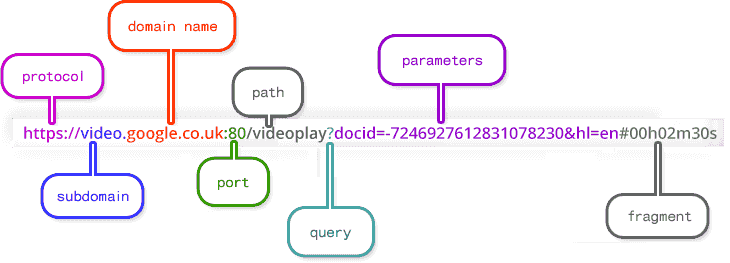
\includegraphics{images/complex_url.png}
\caption{\label{fig:urlanatomy}General url Anatomy, \citet{Anatomyo72} source}
\end{figure}

The \emph{domain name} in red in figure \ref{fig:urlanatomy}, with a specific ID, indicates the server name where the interest resource is stored. The domain name is sometimes accompanied with the \emph{port} whose main role is to point to the open door where data transportation happens. Default port for Transmission Control Protocol ( \emph{TCP} ) is 80. In the following chapter ports will play a crucial role since a compose file wiill instruct containers (\ref{docker}) to open and route communication through these channels and then converge the whole traffic into a secured one \ref{nginx}.
Typically domain name are designed to be human friendly, indeed any domain name has its own proprietary IP and public IP (IPv4 and IPv6) address which is a complex number, e.g.~local machine IP is 95.235.246.91. Here intervenes \emph{DNS} whose function is to redirect domain name to IP and vice versa. The path specifies where the requested resource is located on the server and typically refers to a file or directory. Moving towards folders requires name path locations separated by slashes. In certain scenarios, URLs provide additional \emph{path} information that allows the server to correctly process the request. The URL of a dynamic page (those of who are generated from a data base or user-generated web content) sometimes shows a \emph{query} with one or more parameters followed by a question mark. \emph{Parameters} follow a ``field=value'' scheme each of which is separated by a ``\&'' character for every different parameter field, 6th character from the end in figure \ref{fig:urlanatomy} parameter space. Each further parameter field added is appended at the end of the url string enabling complex and specific search queries.
\emph{Fragments} are an internal page reference often referred to as an anchor. They are typically at the end of a URL, starting with a hash (\#) and pointing to specific part of a HTML document. Note that this is a full browser client-side operation and fragments are used to display only certain parts of already rendered website.
The easiest way of collecting information from websites often involves inspecting and manipulating URLs which refer to the content requested. Therefore urls are the starting point for any scraper and they are also the only functional argument to be feeding to. Url parameters indeed help to route web clients to the requested information and this is done \emph{under the hood} and unconsciously while the user is randomly browsing the web page.
Let us assume to express the necessity to scrape only certain information from a generic website.
Then if this data to be scraped can be circumscribed by properly setting url parameters, under those circumstances it is also demanded a way to consciously compose these urls. In other words a function (or a sevice) needs to mould urls by mimicking their mutations operated by browser while the user is navigating. As a matter of fact as filters (i.e.~parameters) are applied to the initial search page for immobiliare.it then parameters populate the navigation bar. For each of the filters specified a new parameter field and its own selected value are appended to the url string according to the website specific \emph{semantic}. Each website has its own sematic.
As an example are applied directly to the domain name \passthrough{\lstinline!https://www.immobiliare.it/!} the following filters (this is completely done in the dedicated panel):

\begin{itemize}
\tightlist
\item
  rental market (the alternative is selling)
\item
  city is Milan
\item
  bathrooms must be 2
\item
  constrained zones search on ``Cenisio'' and ``Fiera''
\end{itemize}

The resulting url is:

\begin{figure}
\centering
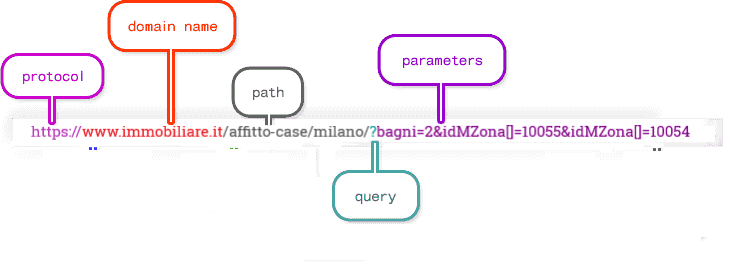
\includegraphics{images/immobiliare_url.png}
\caption{\label{fig:urlanatomy}immobiliare url composed according to some filters, author's source}
\end{figure}

At first glance immobiliare.it does not enact a \emph{clean url} \citep{wiki:cleanurl} structure, which ultimately would simplify a lot the reverse sematic process.
In truth parameters follows a chaotic semantic. While the filter city=``milano'' is located in the url path the remaining are transferred to the url parameters. For some of them the logical trace back from the parameter field-value to their exact meaning is neat, i.e.~bagni=2 and can be said clean. Unfortunately for the others the sematinc is not obvious and requires a further reverse layer to deal with.
In addition to this fact the url in figure \ref{fig:urlanatomy} readdress to the very first page of the search meeting the filter requirements, which groups the first 25 rental advertisements. The following set of 25 items can be reached by relocating the url address to:
\passthrough{\lstinline!https://www.immobiliare.it/affitto-case/milano/?bagni=2\&idMZona[]=10055\&idMZona[]=10054\&pag=2!}. The alteration regards the last part of the url and constitutes a further url parameter field to look for. Note that the first url does not contain ``\&pag=1''. For each page browsed by the user the resulting url happen to be the same plus the prefix ``\&pag='' glued with the correspondent \(n\) page number (from now on referred as \emph{pagination}). This is carried on until pagination reaches either a stopping criteria argument or the last browsable web page (pagination sets as default option 10 pages, which returns a total of 250 rental advertisement).
Therefore for each reversed semantic url are obtainable 25 different links, see figure \ref{fig:nestedstructure} that is where actually are disclosed relevant data and the object of scraping. Links belonging to the 25 items set share the same anatomy: \passthrough{\lstinline!https://www.immobiliare.it/annunci/84172630/!} where the last \emph{path} is associated to a unique
ID, characteristic of the rental property. Unfortunately there is not any available solution to retrieve all the existing ID, therefore links needs to collected directly from ``main'' url in figure \ref{fig:urlanatomy} as an obvious choice.

\begin{figure}
\centering
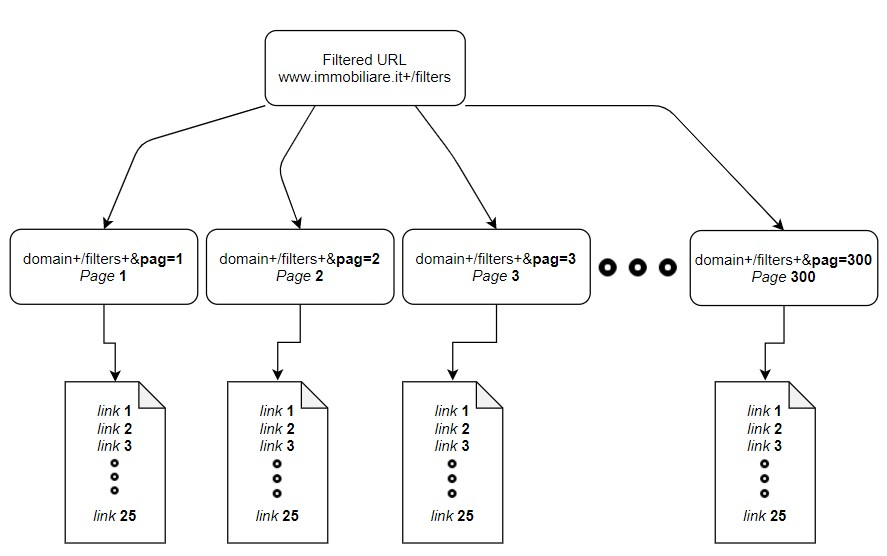
\includegraphics{images/website_tree1.jpg}
\caption{\label{fig:nestedstructure}immobiliare.it website structure, author's source}
\end{figure}

Therefore 4 steps are required to \emph{reverse engineer} the url \citeyearpar{automateddatacollection} and to ultimately make the links access available:

\begin{enumerate}
\def\labelenumi{\arabic{enumi}.}
\tightlist
\item
  Determine how the URL syntactic works for each parameter field
\item
  Build the url based on the reverse engineered sematic:

  \begin{enumerate}
  \def\labelenumii{\alph{enumii}.}
  \tightlist
  \item
    those ones who need an ID parameter value
  \item
    clean ones who need to only explicit the parameter value
  \end{enumerate}
\item
  Pagination is applied to the url until stopping criteria are met
\item
  Obtain the links for each urls previously generated
\end{enumerate}

Once identified the inner composition mechanism by an insistent trial and error then the url restoration could starts. Parameter values for those that requires an ID in figure \ref{fig:urlanatomy} are encoded is a way that each number is associated to its respective zone ID e.g.~as in figure \ref{fig:urlanatomy} ``Fiera'' to 10055 or ``Cenisio'' to 10054. Therefore a decoding function should map the parameter value number back to the correspondent human understandable name e.g from 10055 to ``Fiera'' or 10054 to ``Cenisio'', the exactly opposite logical operation. The decoding function exploits a JSON database file that matches for each ID its respective zone name exploiting suitable JSON properties. The JSON file is previously compounded by generating a number of random url queries and subsequently assigning the query names to their respective ID. As soon as the JSON file is populated the function can take advantage of that database and compose freely urls at need. Pagination generates a set of urls based on the number of pages requested. In the end for each urls belonging to the set of urls, links are collected by a dedicated function and stored into a vector. Furthermore if the user necessitate to directly supply a precomposed url the algorithm overrides the previous object and applies pagination on the provided url. The pseudocode in figure \ref{fig:pseudocode3} paints the logic behid the reverse egineering process.

\begin{figure}
\centering
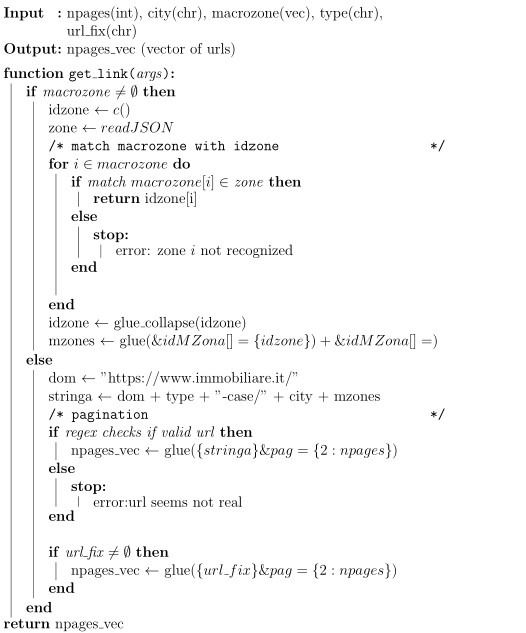
\includegraphics[width=0.7\textwidth,height=\textheight]{images/pseudocode_latex/pseudocode_get_link.jpg}
\caption{\label{fig:pseudocode3}pseudo code algorithm to reverse engineer url, author's source}
\end{figure}

\hypertarget{scraping-with-rvest}{%
\subsection{\texorpdfstring{Scraping with \texttt{rvest}}{Scraping with rvest}}\label{scraping-with-rvest}}

Reverse engineered urls are then feeded to the scraper which arranges the process of scraping according to the flow chart imposed by \passthrough{\lstinline!rvest!} in figure \ref{fig:rvestflowchart}. The sequential path followed is highlighted by the light blue wavy line and offers one solution among all the alternative ways to get to the final content. The left part with respect to the central dashed line of figure \ref{fig:rvestflowchart} takes care of setting up the session and parsing the response. As a consequence at first scraping in consistent way requires to open a session class object with \passthrough{\lstinline!html\_session!}. Session arguments demands both the target url, as built in \ref{fig:pseudocode3} and the request headers that the user may need to send to the web server. Data attached to the web server request will be further explored later in section\ref{spoofing}, tough they are mainly 4: User Agents, emails references, additional info and proxy servers. The session class objects contains a number of useful data regarding either the user log info and the target website such as: the url, the response, cookies, session times etc. Once the connection is established (response 200), functions that come after the opening rely on the object and its response. In other words while the session is happening the user will be authorized with the already provided headers data. As a result jumps from a link to the following within the same session are registered by in the object. Most importantly sessions contain the xml/html content response of the webpage, that is where data needs to be accessed.

\begin{figure}
\centering
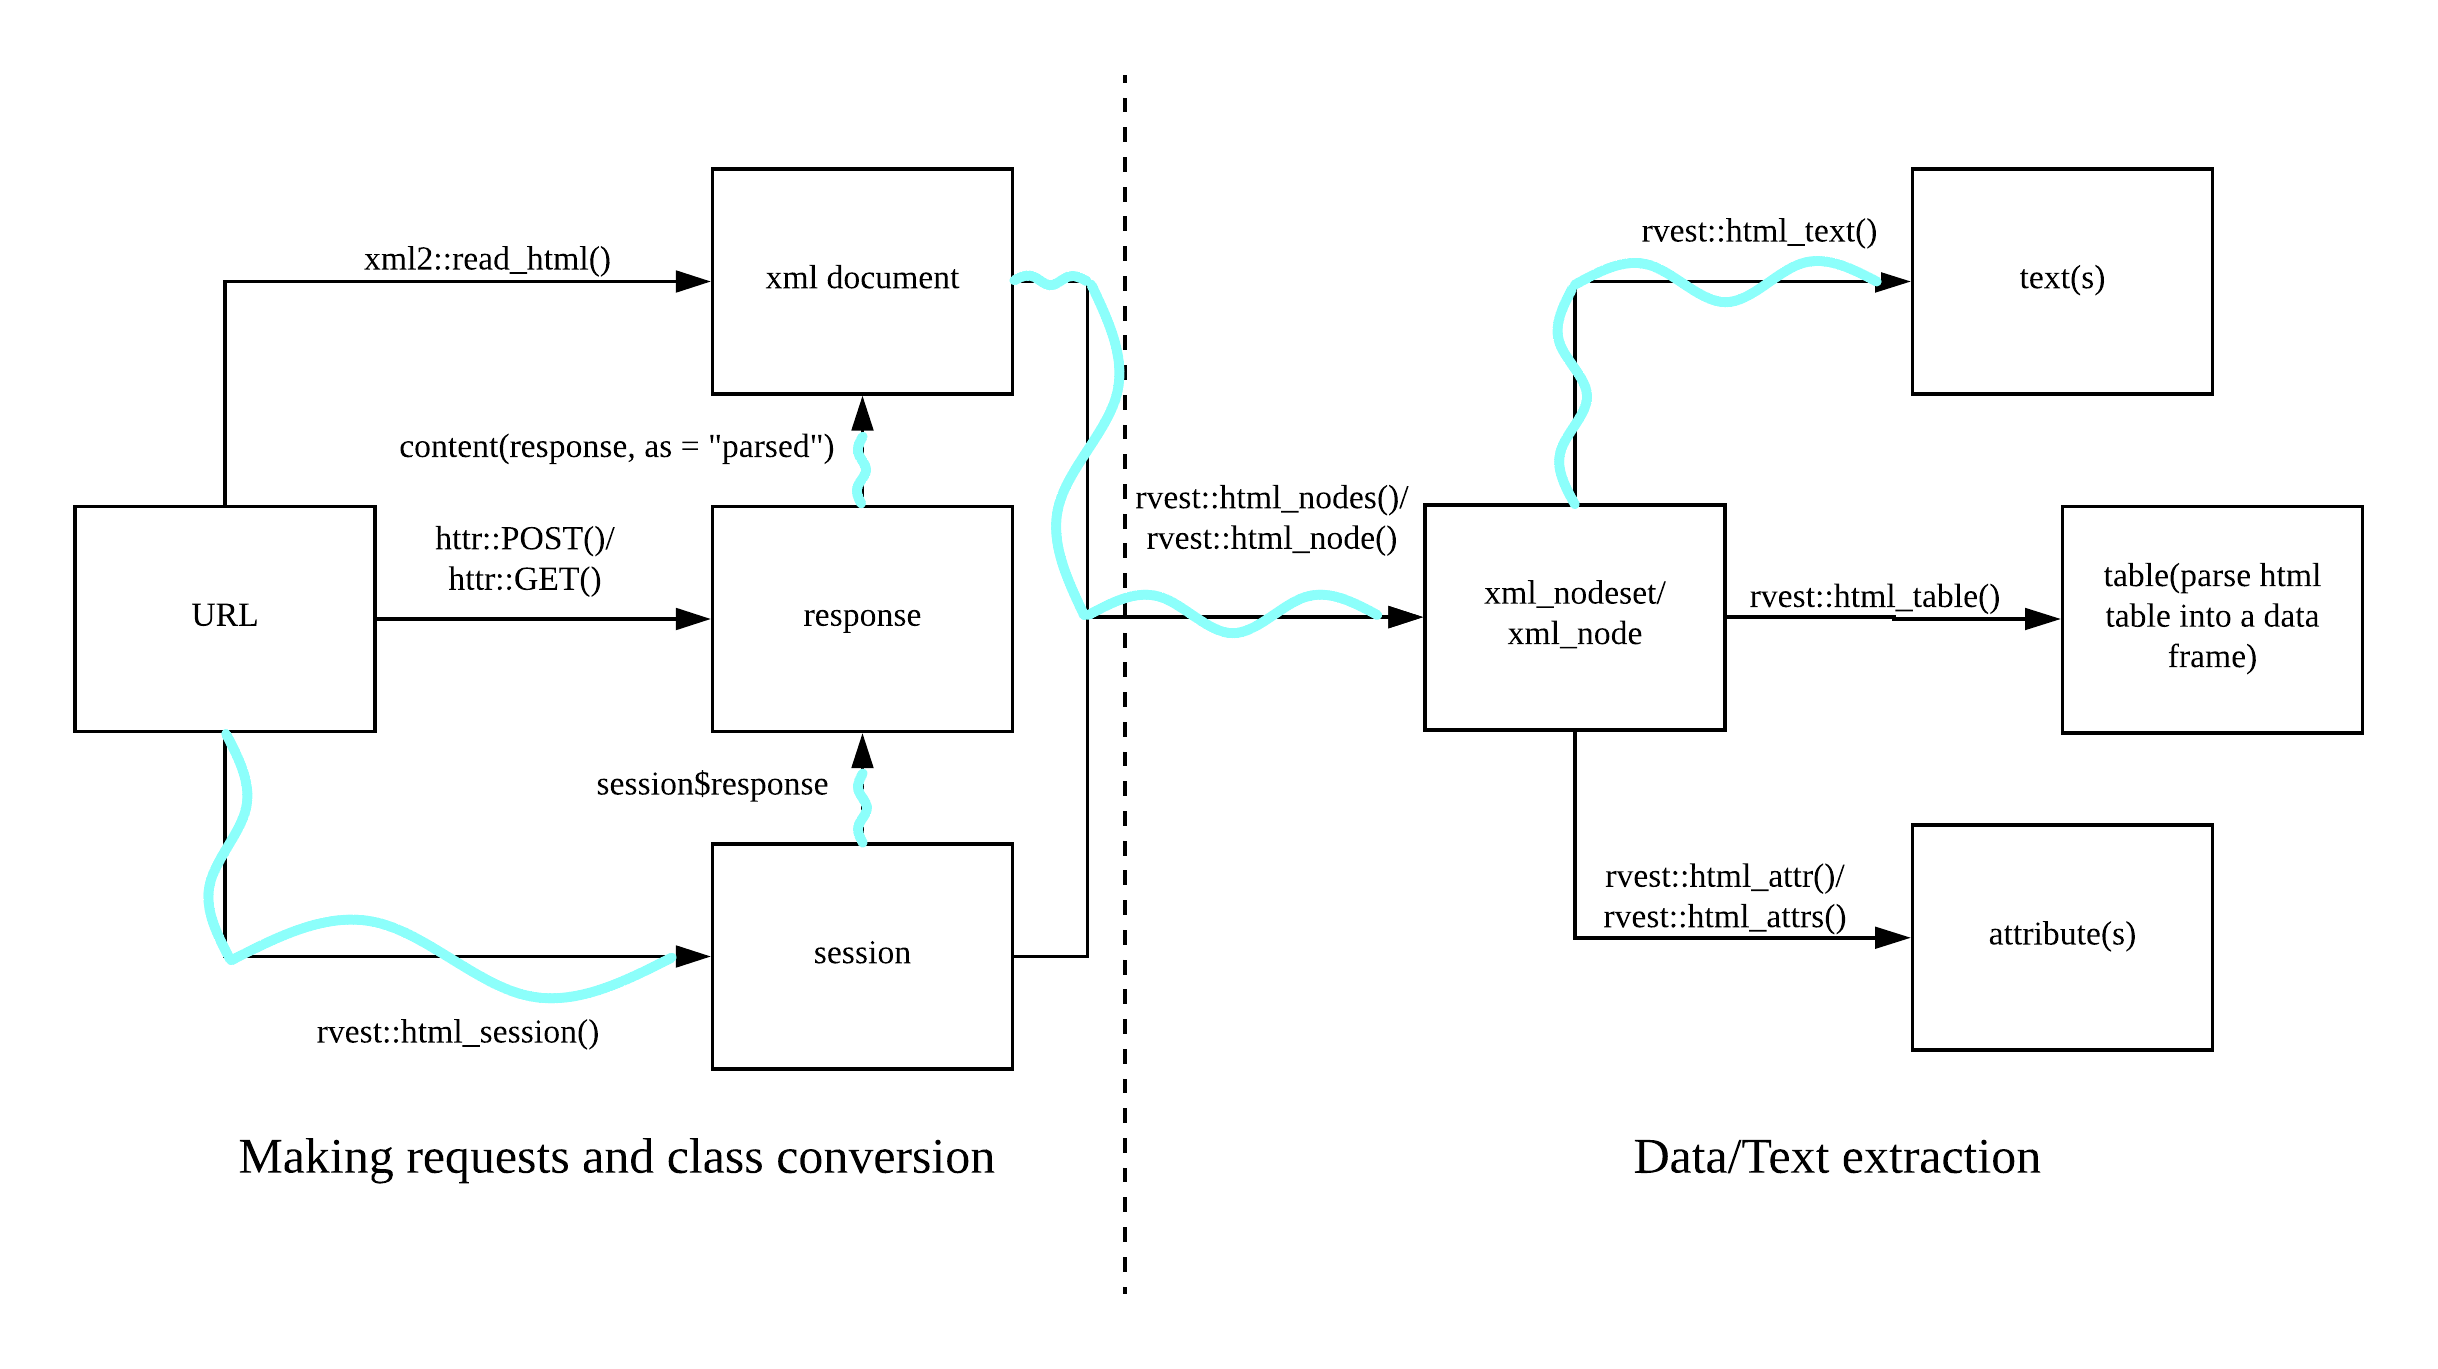
\includegraphics{images/workflow.png}
\caption{\label{fig:rvestflowchart}rvest general flow chart, author's source}
\end{figure}

Indeed at the right of dashed line in \ref{fig:rvestflowchart} are represented the last two steps configured into two \passthrough{\lstinline!rvest!}\citep{rvest} functions that locate the data within the HTML nodes and convert it into a human readble text, i.e.~from HTML/XML to text. The most of the times can be crafty to find the exact HTML node or nodes set that contains the data wanted, expecially when HTML trees are deep nested and dense. html\_node function provides and argument that grants to specify a simple CSS/XPATH selector which may group a set of HTML/XML nodes or a single node. Help comes from an open source library and browser extension technology named SelectorGadget. SelectorGadget \citep{Selectorgadget} which is a JavaScript bookmark that allows to interactively explore which CSS selector is needed to gather desired components from a webpage. Data can be repeated many times into webpages so the same information can be found at multiple CSS queries. This fact highlights one of the priciples embodied in the follwing section \ref{ProperScraping} accroding to which searching methods gravitates. Once the CSS query points address to the desired content then data finally needs to be converted into text. This is what explicitly achieve html\_text.

\hypertarget{ProperScraping}{%
\section{Searching Technique for Scraping}\label{ProperScraping}}

The present algorithm in figure \ref{fig:pseudocode1} imposes a nested sequential search strategy and gravitates around the fact that data within the same webpage is repeated many times, so there exist multiple CSS selections for the exact same information. Furthermore since data is repeated has also less probability to be missed. CSS sequential searches are calibrated from the highest probability of appearance in that CSS selector location to the lowest so that most visited locations are also the the most likely to grab data.
A session object \passthrough{\lstinline!opensess!}, the one seen in \ref{fig:rvestflowchart}), is initialized sending urls built in \ref{fig:pseudocode3}. The object opensess constitutes a check point obj because it is reused more than once along the algorithm flow. The object contains session data as well as HTML/XML content. Immediately after another object \passthrough{\lstinline!price!} parses the sessions and points to a CSS query through a set of HTML nodes. The CSS location \passthrough{\lstinline!.im-mainFeatures\_\_title!} addresses a precise group of data which are found right below the main title. Expectations are that monthly price amount in that location is a single character vector string, containing price along with unnecessary non-UTF characters. Then the algorithm bumps into the first \passthrough{\lstinline!if!} statement. The logical condition checks whether the object \passthrough{\lstinline!price!} first CSS search went lost. If it does not the algorithm directly jumps to the end of the algorithm and returns a preprocessed single quantity. Indeed if it does it considers again the check point \passthrough{\lstinline!opensess!} and hits with a second css query \passthrough{\lstinline!.im-features\_\_value , .im-features\_\_title!}, pointing to a second data location. Note that the whole search is done within the same session (i.e.~reusing the same session object), so no more additional request headers \ref{spoofing} has to be sent). Since the second CSS query points to data sequentially stored into a list object, the newly initialized \passthrough{\lstinline!price2!} is a type list object containing various information. Then the algorithm flows through a second \passthrough{\lstinline!if!} statement that checks whether \passthrough{\lstinline!"prezzo"!} is matched in the list, if it does the algorithm returns the +1 position index element with respect to the ``prezzo'' position. This happens because data in the list are stored by couples sequentially (as a flattened list), e.g.~list(title, ``Appartamento Sempione'', energy class, ``G'', ``prezzo'', 1200/al mese). Then in the end a third CSS query is called and a further nested if statement checks the emptiness of the latest CSS query. \passthrough{\lstinline!price3!} points to a hidden JSON object within the HTML content. If even the last search is lost then the algorithm escapes in the else statement by setting \passthrough{\lstinline!NA\_Character\_!}, ending with any CSS query is able to find price data.
The search skeleton used for price scraping constitutes a standard reusable search method in the analysis for all the scraping functions. However for some of the information not all the CSS location points are available and the algorithm is forced to be rooted to only certain paths, e.g.~``condizionatore'' can not be found under main title and so on.

\begin{figure}
\centering
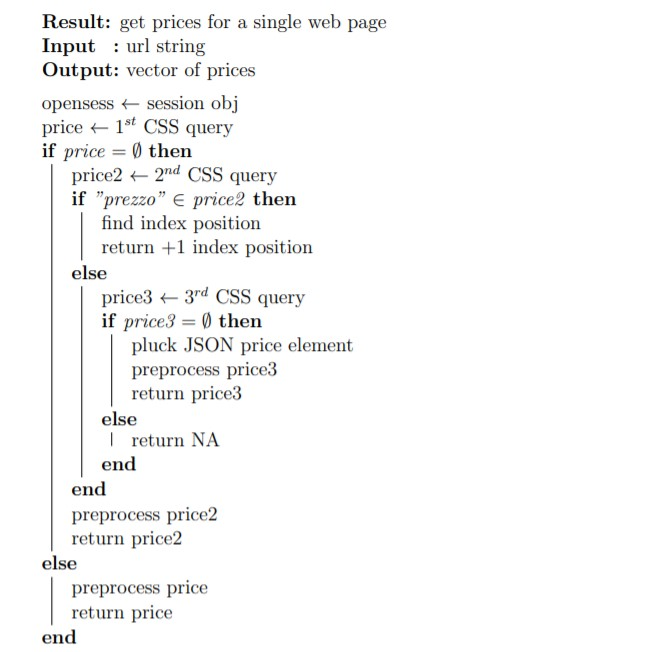
\includegraphics[width=0.7\textwidth,height=\textheight]{images/pseudocode_latex/pseudocode_price.jpg}
\caption{\label{fig:pseudocode1}pseudo code algorithm for price search, author's source}
\end{figure}

Once all the functions have been designed and optimized with respect to their scraping target they need to be grouped into a single ``main'' \emph{fastscrape} function, figure \ref{fig:pseudocode4}. This is accomplished into the API function endpoint addressed in section \ref{plumberapi}, which also applies some sanitization, next chapter section \ref{sanitize}, on users inputs and administers also some security API measures, as in \ref{DoS} outside the main function. Moreover as it will be clear in section \ref{parallelscraping} the parallel back end will be registered outside the scraping function for unexplained inner functioning reasons.

\begin{figure}
\centering
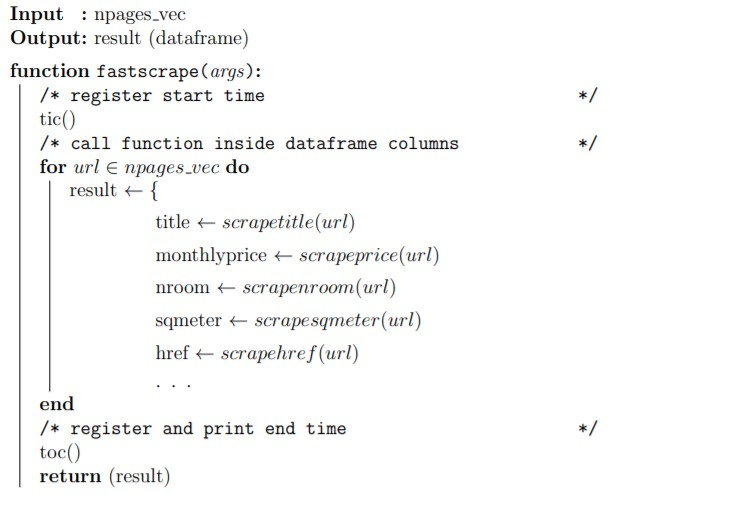
\includegraphics{images/pseudocode_latex/pseudocode_mainjpg.jpg}
\caption{\label{fig:pseudocode4}pseudo code algorithm structure for fatstscrape, author's source}
\end{figure}

\textbf{pseudo code}

\hypertarget{best-practices}{%
\section{Scraping Best Practices and Security provisions}\label{best-practices}}

Web scraping have to naturally interact multiple times with both the \emph{client} and \emph{server side} and as a result many precautions must be seriously taken into consideration. From the server side a scraper can forward as many requests as it could (in the form of sessions opened) which might cause a traffic bottleneck (DOS attack \citet{wiki:DOS}) impacting the overall server capacity. As a further side effect it can confuse the nature of traffic due to fake user agents \ref{spoofing} and proxy servers, consequently analytics reports might be driven off track.
Those are a small portion of the reasons why most of the servers have their dedicated Robots.txt files. Robots.txt \citet{meissner_2020} are a way to kindly ask webbots, spiders, crawlers to access or not access certain parts of a webpage. The de facto ``standard'' never made it beyond a \emph{informal} ``Network Working Group internet draft''. Nonetheless, the use of robots.txt files is widespread due to the vast number of web crawlers (e.g.~\href{https://en.wikipedia.org/robots.txt}{Wikipedia robot}, \href{https://www.google.com/robots.txt}{Google robot}). Bots from the own Google, Yahoo adhere to the rules defined in robots.txt files, although their \emph{interpretation} might differ.

Robots.txt files \citep{robotstxt} essentially are plain text and always found at the root of a website's domain. The syntax of the files follows a field-name value scheme with optional preceding user-agent. Blocks are separated by blank lines and the omission of a user-agent field (which directly corresponds to the HTTP user-agent field, cleared later in \ref{spoofing}) is seen as referring to all bots. The whole set of possible field names are pinpointed in \citet{google:robottxt}, some important are: user-agent, disallow, allow, crawl-delay, sitemap and host. Some common standard interpretations are:

\begin{itemize}
\tightlist
\item
  Finding no robots.txt file at the server (e.g.~HTTP status code 404) implies full permission.
\item
  Sub-domains should have their own robots.txt file, if not it is assumed full permission.
\item
  Redirects from subdomain www to the domain is considered no domain change - so whatever is found at the end of the redirect is considered to be the robots.txt file for the subdomain originally requested.
\end{itemize}

A comprehensive scraping library that observes a web etiquette is the \passthrough{\lstinline!polite!} \citep{polite} package. Polite combines the effects of \passthrough{\lstinline!robotstxt!}, \passthrough{\lstinline!ratelimitr!} \citeyearpar{ratelimitr} to limit sequential session requests together with the \passthrough{\lstinline!memoise!} \citep{memoise} for robotstxt response caching. Even though the solution meets the politeness requirements (from server and client side) ratelimitr is not designed to run in parallel as documented in the vignette \citep{ratelimitr}. This is a strong limitation as a result the library is not applied. However the 3 simple but effective web etiquette principles around, which is the package wrapped up, describe what are the guidelines for a ``polite'' session:

\begin{quote}
The three pillars of a polite session are seeking permission, taking slowly and never asking twice.

\hfill --- Dmytro Perepolkin, polite author
\end{quote}

The three pillars constituting the \emph{Ethical} web scraping manifesto \citep{densmore_2019} are considered as common shared \emph{best practices} that are aimed to self regularize scrapers. In any case these guidelines have to be intended as eventual practices and by no means as required by the law. However many scrapers themselves, as website administrators or analyst, have been fighting for many and almost certainly coming years with bots, spiders and derivatives. As a matter of fact intensive scraping might fake out real client navigation logs and confuse digital footprint, which results in induced distorted analytics. On the other hand if data is not given and APIs are not available, then scraping is sadly no more an option.
Therefore throughout this analysis the goal will be trying to find a well balanced trade-off between interests on the main actors involved.
Newly balanced (with respect to the author thought) guidelines would try to implement at first an obedient check on the validity of the path to be scraped through a cached function. Secondly it will try to limit request rates to a more feasible time delay, by keeping into the equation also the client time constraints. In addition it should also guarantee the continuity in time of scraping not only from the possibility to fail section \ref@(possibly)), but also from servers ``unfair'' denial (in section \ref{spoofing}).
With that said a custom function caches the results of robotstxt into a variable i.e.~\passthrough{\lstinline!polite\_permission!}. Then paths allowed are evaluated prior any scraping function execution. Results should either negate or affirm the contingency to scrape the following url address.

\begin{lstlisting}
#> Memoised Function:
#> [1] TRUE
\end{lstlisting}

\passthrough{\lstinline!polite\_permission!} is then reused to check, if any, the server suggestion on crawl relay. In this particular context no delays are kindly advised. As a default polite selection delay request rates are set equal to 2.5 seconds. Delayed are managed through the \passthrough{\lstinline!purrr!} stack. At first a \passthrough{\lstinline!rate!} object is initialized based on polite\_permission results, as a consequence a \passthrough{\lstinline!rate\_sleep!} delay is defined and iterated together with any request sent, as in \citet{rate_delay}.

\begin{lstlisting}[language=R]
get_delay = function(memoised_robot, domain) {
  
  message(glue("Refreshing robots.txt data for %s... {domain}"))
  temp  = memoised_robot$crawl_delay
  
  if (length(temp) > 0 && !is.na(temp[1,]$value)) {
    star = dplyr::filter(temp, useragent=="*")
    if (nrow(star) == 0) star = temp[1,]
    as.numeric(star$value[1])
  } else {
    2.5L
  }
  
}
get_delay(rbtxt_memoised, domain = dom)
#> [1] 2.5
\end{lstlisting}

\hypertarget{HTTPmethod}{%
\section{HTTP overview}\label{HTTPmethod}}

URLs in browsers as in \ref{reverse} are a way to access to web content whether this accounts for getting from one location to the following, or checking mails, listening to musics or downloading files. However Internet communication is a stratification of layers conceived to make the whole complex system working. In this context URLs are the layer responsible for \emph{user interaction}. The rest of the layers which involve techniques, standards and protocols, are called in ensemble Internet Protocols Suite ( \emph{IPS} ) \citeyearpar{automateddatacollection}. The TCP (Transmission Control Protocol) and IP (Internet Protocol) are two of the most important actors on the IP Suite and their role is to represent the \emph{Internet layer} (IP) and the \emph{transportation layer} (TCP). In addition they also guarantee trusted transmission of data. Inner properties and mechanism are beyond the scope of the analysis, luckily they are not required in this context. Resting on the transportation layer there are specialized message exchange protocols such as the HTTP (Hyper Text Transfer Protocol), FTP (File Transfer Protocol). In addition, there may be also e-mail exchange protocols for transmission, such as Post Office Protocol (POP) for Email Recovery and for storage and retrieval, IMAP (Internet Message Acccess Protocol). The aforementioned protocols describe default vocabulary and procedures to address particular tasks for both clients and servers and they can be ascribed to the transportation layer. HTTP is the most widespread, versatile enough to ask for almost any resource from a server and can also be used to transfer data to the server rather than to recover. In figure \ref{fig:httpschema} is painted a schematized version of a User-Server general HTTP communication/session. If a website e.g.~\href{https://www.immobiliare.it/}{immobiliare.it} is browsed from a web browser e.g.~Chrome (the HTTP client) then the client is interrogating a Domain Name System (DNS) which IP address is associated with the domain part of the URL. When the browser has obtained the IP address as response from the DNS server then connection/session is established with HTTP server via TCP/IP. From a content perspective data is gathered piece-by-piece, if the content is not exclusively HTML then the the browser client renders the content as soon as it receives data.

\begin{figure}
\centering
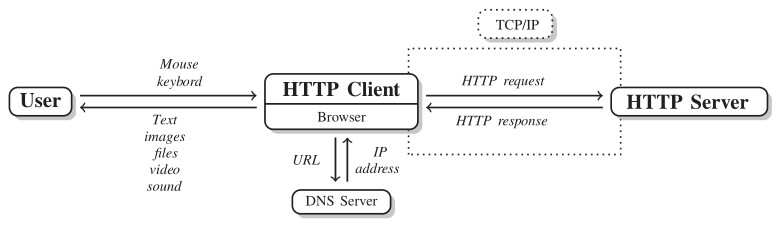
\includegraphics{images/http_schema.jpg}
\caption{\label{fig:httpschema} User-Server communication scheme via HTTP, source \citet{automateddatacollection}}
\end{figure}

Furthermore HTTP should be borne in mind two essential facts.

\begin{itemize}
\tightlist
\item
  HTTP is not only a hypertext protocol, but it is used for all sorts of services (i.e.~APIs)
\item
  HTTP is a \emph{stateless} protocol, which means that response and request and the the resulting interaction between client and server is managed by default as it were the first time they connected.
\end{itemize}

\emph{HTTP messages} consist of three sections -- start line, \emph{headers} and body -- whether client requests or server response messages. The start line of the server response begins with a declaration on the highest HTTP version. The header underneath the start line contains client and server meta data on the preferences for content displaying. Headers are arranged in a collection of name-value pairs.
The body of an HTTP message contains the content of the response and can be either binary or plain text. Predominantly in the context of the analysis are headers which are the fields where lay the definition of the actions to take upon receiving a request or response. For what concerns the analysis the focus is on \emph{identification headers} (both in request and response) whose role is to describe user preferences when sessions are opened i.e.~default language, optimization of content display throughout devices. The exploited ones are:

(metti anche altra roba da altre fonti)

\begin{itemize}
\tightlist
\item
  \emph{Authorization} (request): authentication field allows to insert personal credentials to access to dedicated content (log in to the immobiliare.it account). Credentials in requests are not really encrypted, rather they are encoded with Base64. Therefore they can be easily exposed to security breaches, which it does not happen when using HTTP (HTTP Security) that applies encryption to basic authentication, extensively presented in \ref{HTTPS}.
\item
  \emph{Set-Cookie} (response): Cookies allow the server to keep user identity. They are a method to transform \emph{stateless HTTP} communication (second point in previous ) into a secure discussion in which potential answers rely on past talks.
\item
  \emph{User-Agent} (request), faced in next section \ref{spoofing}.
\end{itemize}

\hypertarget{spoofing}{%
\subsection{User Agent and further Identification Headers Spoofing}\label{spoofing}}

\begin{definition}[User Agents]
\protect\hypertarget{def:useragents}{}{\label{def:useragents} \iffalse (User Agents) \fi{} }The user Agent (from now on refered as UA) ``retrieves, renders and facilitates end-user interaction with Web content'' \citep{UaDef}.
\end{definition}

In the HTTP identification headers the UA string is often considered as \emph{content negotiator} \citep{wiki:UserAgent}. One the basis of the UA, the web server can negotiate different CSS loadings, custom JavaScript delivery or it can automatically translate content on UA language preferences \citep{whoishostingthis.com}.
UA is a dense content string that includes many User details: the user application or software, the operating system (and versions), the web client, the web client's version, as well as the web engine responsible for content displaying (e.g.~AppleWebKit). When the request is sent from an application software as R (no web browser), the default UA is set as:

\begin{lstlisting}
#> [1] "libcurl/7.64.1 r-curl/4.3 httr/1.4.2"
\end{lstlisting}

Indeed when a request comes from a web browser a full UA example and further components breakdown is (current machine):

\passthrough{\lstinline!Mozilla/5.0 (Windows NT 6.3; WOW64) AppleWebKit/537.36 (KHTML, like Gecko) Chrome/45.0.2454.85 Safari/537.36!}

\begin{itemize}
\tightlist
\item
  The browser application is Mozilla build version 5.0 (i.e.~`Mozilla-compatible').
\item
  The Operating System is Windows NT 6.3; WOW64, running on Windows.
\item
  The Web Kit provides a set of core classes to display web content in windows \citep{UserAgen23}, build version 537.36.
\item
  The Web Browser is Chrome version 45.0.2454.85.
\item
  The client is based on Safari, build 537.36.
\end{itemize}

The UA string is also one of the main responsible according to which Web crawlers and scrapers through a dedicated name field in robotstxt \ref{best-practices} may be ousted from accessing certain parts of a website. Since many requests are sent the web server may encounter insistently the same UA (since the device from which they are sent is the same) and as consequence it may block requests associated to the own UA. In order to avoid server block the scraping technique adopted in this analysis rotates a pool of UAs. That means each time requests are sent a different set of headers are drawn from the pool and then combined. The more the pool is populated the larger are the UA combinations. The solution proposed tries in addition to automatically and periodically resample the pool as soon as the website from which U agents ID are extracted updates newer UA strings.

\begin{lstlisting}[language=R]
set.seed(27)
url = "https://user-agents.net/"
agents = read_html(url) %>%
  html_nodes(css = ".agents_list li") %>% 
  html_text()

agents[sample(1)]
#> [1] "Mozilla/5.0 (Linux; Android 8.1.0; INE-LX2 Build/HUAWEIINE-LX2; wv) AppleWebKit/537.36 (KHTML, like Gecko) Version/4.0 Chrome/88.0.4324.152 Mobile Safari/537.36 [FB_IAB/FB4A;FBAV/305.1.0.40.120;]"
\end{lstlisting}

The same procedure has been applied to the From identification header attached to the request. E-mails, that are randomly generated from a website, are scraped and subsequently stored into a variable. A further way to imagine what this is considering low level API calls to dedicated servers nested into a more general higher level API.
However UA field name technology has been recently sentenced as superseded in favor of a newer (2020) proactive content negotiator named \emph{Hints} \citet{wiki:UserAgentHints}.

An even more secure approach may be accomplished rotating proxy servers between the back and forth sending-receiving process.
\begin{definition}[Proxy Server]
\protect\hypertarget{def:proxy}{}{\label{def:proxy} \iffalse (Proxy Server) \fi{} }A proxy server is a gateway between the web user and the web server.
\end{definition}
While the user is exploiting a proxy server, internet traffic in the form of HTTP request, figure \ref{fig:proxycommunication} flows through the proxy server on its way to the HTTP server requested. The request then comes back through that same proxy server and then the proxy server forwards the data received from the website back to the client.
Form a user perspective benefits regards:

\begin{itemize}
\tightlist
\item
  anonymity on the Web
\item
  overcome restriction access to IPs imposed to requests coming from certain locations
\end{itemize}

Many proxy servers are offered as paid version. In this particular case security barrijers are not that high and this suggests to not apply them. As a further disclaimer many online services are providing free proxies server access, but this comes at a personal security cost due to a couple of reasons:

\begin{figure}
\centering
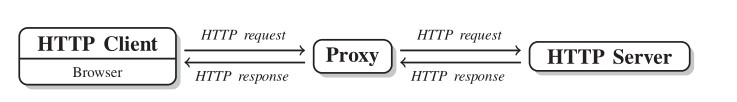
\includegraphics{images/proxy_schema.jpg}
\caption{\label{fig:proxycommunication} proxy middle man,, source \citet{automateddatacollection}}
\end{figure}

\begin{itemize}
\tightlist
\item
  Free plan Proxies are shared among a number of different clients, so as long as someone has used them in the past for illegal purposes the client is indirectly inheriting their legal infringements.
\item
  Very cheap proxies, for sure all of the ones free, have the activity redirected on their servers monitored, profiling in some cases a user privacy violation issue.
\end{itemize}

\hypertarget{possibly}{%
\section{Dealing with failure}\label{possibly}}

During scraping many difficulties coming from different source of problems are met. Some of them may come from the website's layout changes (\ref{ProperScraping}), some of them may regard internet connection, some other may have been caused by security breaches (section \ref{spoofing}).
One of the most inefficient event it can happen is an unexpected error thrown while sending requests that causes all the data acquired and future coming going lost. In this particular context is even more worrying since scraping ``main'' functions is able to call 34 different functions each of which points to a different data location. Within a single function invocation, pagination contributes to initialize 10 pages. Each single page includes 25 different single links leading to a number of 8500 single data pieces. Unfortunately the probability given 8500 associated to one piece being lost, unparsed is frankly high.
For all the reasons said scraping functions needs to deal with the possibility to fail. This is carried out by the implementation of \passthrough{\lstinline!purrr!} vectorization function \passthrough{\lstinline!map!} (and its derivatives) and the adverb \passthrough{\lstinline!possibly!} \citet{possibly}. \emph{Possibly} takes as argument a function (map iteration over a list) and returns a modified version. In this case, the modified function returns an empty dataframe regardless of the error thrown. The approach is strongly encouraged when functions need to be mapped over large objects and time consuming processes as outlined in \citet{Rdatascience} section 21.6. Moreover vectorization is not only applied to a vector of urls, but also to a set of functions defined in the environemnt.

\begin{figure}
\centering
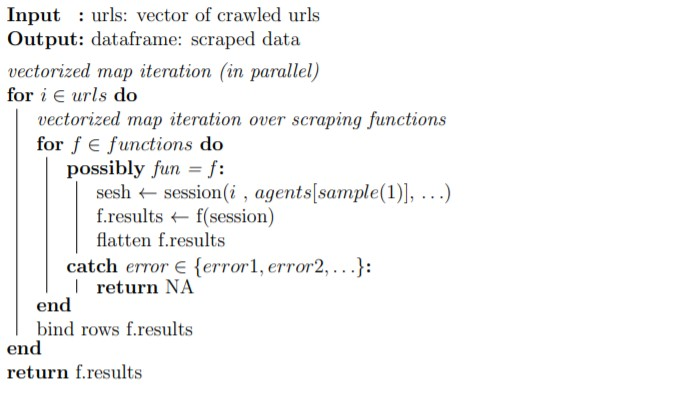
\includegraphics[width=0.7\textwidth,height=\textheight]{images/pseudocode_latex/pseudocode_possibly.jpg}
\caption{\label{fig:pseudocode2}pseudo code for a generic set of functions applied with possibly fail dealers , author's source}
\end{figure}

\hypertarget{parallelscraping}{%
\section{Parallel Scraping}\label{parallelscraping}}

Scraping run time is crucial when dealing with dynamic web pages. This assumption is stronger in Real Estate rental markets where time to market is a massive competitive advantage.
From a run time perspective the dimension of the problem requires as many html session opened as single links crawled (refer to previous section \ref{possibly}). As a result computation needs to be \emph{parallelized} in order to be feasible.
The extraordinary amount of time taken in a non-parallel environment is caused by R executing scraping on a single processor \emph{sequentially} url-by-url in a queue, left part of figure \ref{fig:singlethreaded} (i.e.~single threaded computing).

\begin{definition}[parallel]
\protect\hypertarget{def:parallel}{}{\label{def:parallel} \iffalse (parallel) \fi{} }\emph{Parallel execution} is characterized as multiple operations taking place over overlapping time periods. \citep{eddelbuettel2020parallel}
\end{definition}

This requires multiple execution units and modern processors architecture provide multiple cores on a single processor and a way to redistribute computation (i.e.~multi threaded computing). As a result tasks can be split into smaller chunks over processors and then multiple cores for each processor, right part of figure \ref{fig:singlethreaded}.
Therefore Parallel scraping (sometimes improperly called \href{https://medium.com/@cummingsi1993/the-difference-between-asynchronous-and-parallel-6400729fa897}{asynchronous}) functions are proposed, so that computation do not employ vast cpu time (i.e.~cpu-bound) and space.

\begin{figure}
\centering
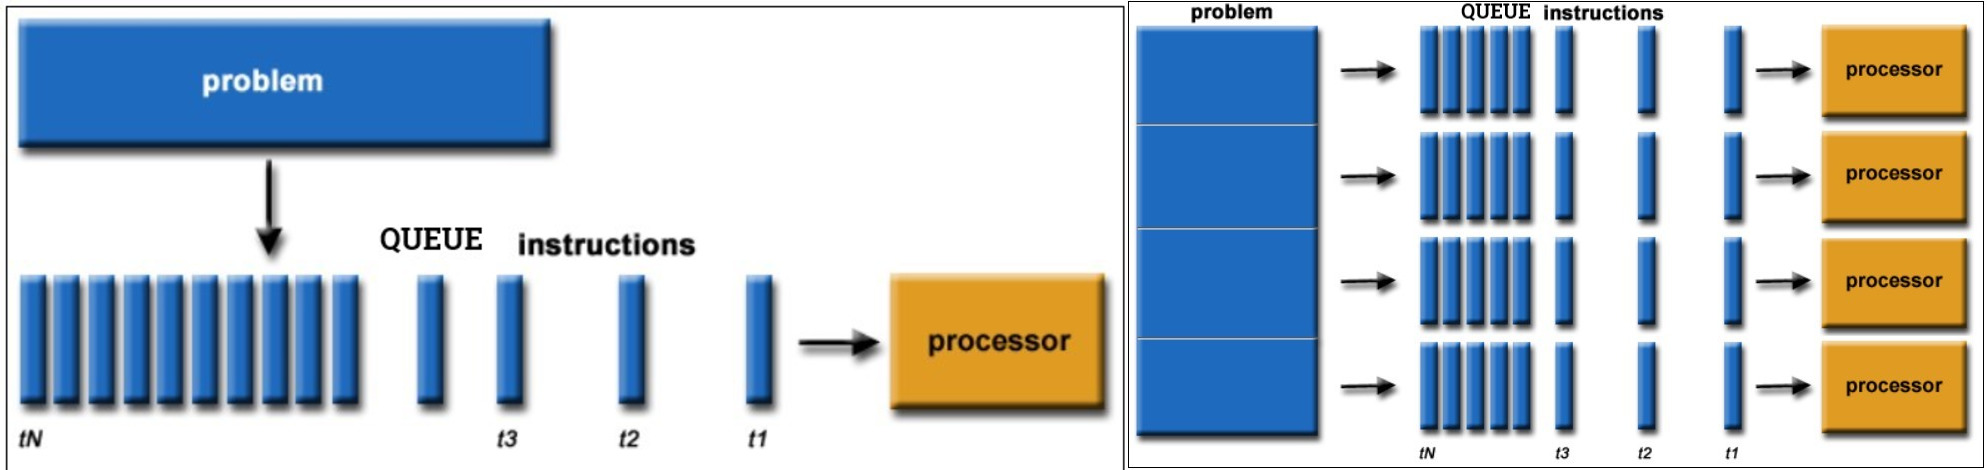
\includegraphics{images/parallel_problem.jpg}
\caption{\label{fig:singlethreaded}single threaded computing vs parallel computing, \citet{barney} source}
\end{figure}

Parallel execution heavily depends on hardware and software choice. Linux environments offers multi-core computation through \emph{forking} \citep{wiki:forking} (only on Linux) so that global variables are directly inherited by child processes. As a matter of fact when computation are split over cores they need to import whatever it takes to be carried out, such as libraries, variables, functions. From a certain angle they need to be treated as a containerized stand-alone environments. This can not happen in Windows (local machine) since it does not support multicore.

\begin{lstlisting}[language=R]
future::supportsMulticore()
#> [1] FALSE
\end{lstlisting}

\emph{Cluster processing} is an alternative to multi-core processing, where parallelization takes place through a collection of separate processes running in the background. The parent R session instructs the dependencies that needs to be sent to the children sessions.
This is done by registering the parallel back end. Arguments to be supplied mainly regards the strategy (i.e.~multi-core cluster, also said multisession) and the \emph{working group}. The working group is a software concept \citep{parallelr}, that points out the number of processes and their relative computing power/memory allocation according to which the task is going to be split. Moreover from a strictly theoretic perspective the \emph{workers} (i.e.~working group single units) can be greater than the number of physical cores detected. Although parallel libraries as a default choice (and choice for this analysis) initializes \emph{as many workers as} physical HT (i.e.~Hyper Threaded) \emph{cores}.
Parallel looping constructor libraries generally pops up as a direct cause of new parallel packages. The latest research activity by Bengtsson \citet{doFuture} indeed tries to unify all the previous back ends under the same umbrella of \passthrough{\lstinline!doFuture!}. The latter library allows to register many back ends for the most popular parallel looping options solving both the dependency inheritance problem and the OS agnostic challenge.
The two alternatives proposed for going parallel are \passthrough{\lstinline!Future!} \citet{future} with \passthrough{\lstinline!furrr!} \citet{furrr} and \passthrough{\lstinline!doFuture!} \citeyearpar{doFuture} along with the \passthrough{\lstinline!foreach!} \citet{foreach} loop constructor. The former is a generic, low-level API for parallel processing as in \citet{bengtsson_2017}. The latter takes inspiration by the previous work and it provides a back-end agnostic version of \passthrough{\lstinline!doParallel!} \citet{doParallel}. Further concepts on parallel computing are beyond the scope of the analysis, some valuable references are \citet{barney} and \citet{parallelr}.

\hypertarget{parallel-furrrfuture}{%
\subsection{Parallel furrr+future}\label{parallel-furrrfuture}}

Simulations are conducted on a not-rate-delayed (section \ref{best-practices}) and restricted set of functions which may be considered as a ``lightweight'' version of the final API scraping endpoint.
As a disclaimer run time simulations may not be really representative to the problem since they are performed on a windows 10, Intel(R) Core(TM) i7-8750H 12 cores RAM 16.0 GB local machine. Indeed the API is served on a Linux Ubuntu distro t3.micro 2 cores RAM 1.0 GB server which may adopt forking. Simulations for the reasons said can only offer a run time performance approximation for both of the parallel + looping constructor combinations.

The first simulation considers \passthrough{\lstinline!furrr!} which enables mapping (i.e.~vectorization with \passthrough{\lstinline!map!}) through a list of urls with \passthrough{\lstinline!purrr!} and parallelization with \passthrough{\lstinline!Future!}. Future gravitates around a programming concept called ``future'', initially introduced in late 70's by Baker \citep{BakerFuture}. Futures are abstractions for values that may be available at a certain time point later \citeyearpar{future}.
These values are result of an evaluated expression, this allows to actually divide the assignment operation from the proper result computation. Futures have two stages \emph{unresolved} or \emph{resolved}. If the value is queried while the future is still unresolved, the current process is blocked until the stage is resolved. The time and the way futures are resolved massively relies on which strategy is used to evaluate them. For instance, a future can be resolved using a \emph{sequential} strategy, which means it is resolved in the current R session. Other strategies registered with \passthrough{\lstinline!plan()!}, such as \emph{multi-core} (on Linux) and \emph{multisession}, may resolve futures in parallel, as already pointed out, by evaluating expressions on the current machine in forked processes or concurrently on a cluster of R background sessions.
With parallel futures the current/main R process does not get ``bottlenecked'', which means it is available for further processing while the futures are being resolved in separate processes running in the background. Therefore with a ``multisession'' plan are opened as many R background sessions as workers/cores on which chunks of futures (urls) are split and resolved in parallel. From an algorithmic point of view It can be compared to \emph{a divide and conquer} strategy where the target urls are at first redistributed among workers/cores (unresolved) through background sessions and then are scraped in equally distributed chunks (resolved).
Furthermore furrr has also a convenient tuning option which can interfere with the redistribution scheduling of urls' chunks over workers. The argument scheduling can adjust the average number of chunks per worker. Setting it equal to 2 brings \emph{dinamicity} \citeyearpar{furrr} to the scheduling so that if at some point a worker is busier then chunks are sent to the more free ones.

\begin{figure}
\centering
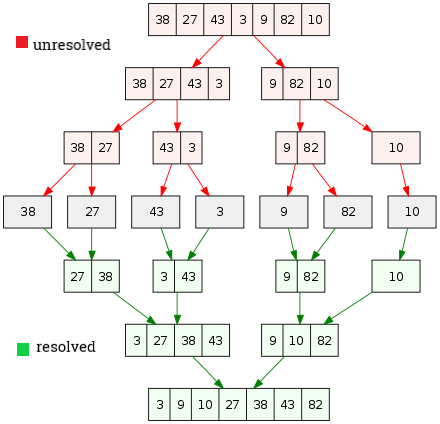
\includegraphics{images/divideconquer.png}
\caption{\label{fig:divideconquer}Futures envisaged as Divide \& Conquer algorithm, author's source}
\end{figure}

The upper plot in figure \ref{fig:furrrfuture} are 20 simulations of 100 url (2500 data points) performed by the lightweight scraping. On the horizontal axis are plotted the 20 simulations and on the vertical axis are represented the respective elapsed times. One major point to breakdown is the first simulation run time measurement which is considerably higher with respect to the others i.e.~15 sec vs mean 7.72 sec.~Empirical demonstrations traces this behavior back to the opening time for all the background sessions. As a result the more are the back ground sessions/workers, the more it would be the time occupied to pop up all the sessions. As opposite whence many sessions are opened the mean execution time for each simulation is slightly less.
The lower plot in in figure \ref{fig:furrrfuture} tries to capture the run time slope behavior of the scraping function when urls (1 to 80) are cumulated one by one. The first iteration scrapes 1 single url, the second iteration 2, the third 3 etc. Three replications of the experiment has been made, evidenced by three colours. The former urls are more time consuming confirming the hypothesis casted before. Variability within the first 40 urls for the three repetitions does not show diversion. However It slightly increases when the 40 threshold is trespassed. Two outliers in the yellow line are visible in the nearby of 50 and 60. One straightforward explanation might be delay in server response. A further point of view may address the workers being overloaded, but no evidences are witnessed on cores activity as in plot \ref{fig:cpumonitor}. The measured computational complexity of scraping when \(n\) is number of urls seems to be much more less than linear \(\mathcal{O}(0.06n)\).

\begin{figure}
\centering
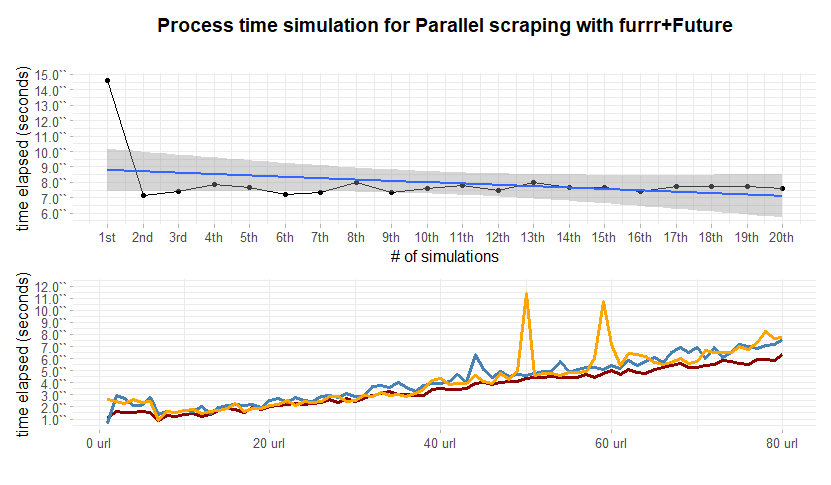
\includegraphics{images/simulations/final_furrr_future.png}
\caption{\label{fig:furrrfuture}computational complexity analysis with Furrr}
\end{figure}

\begin{figure}
\centering
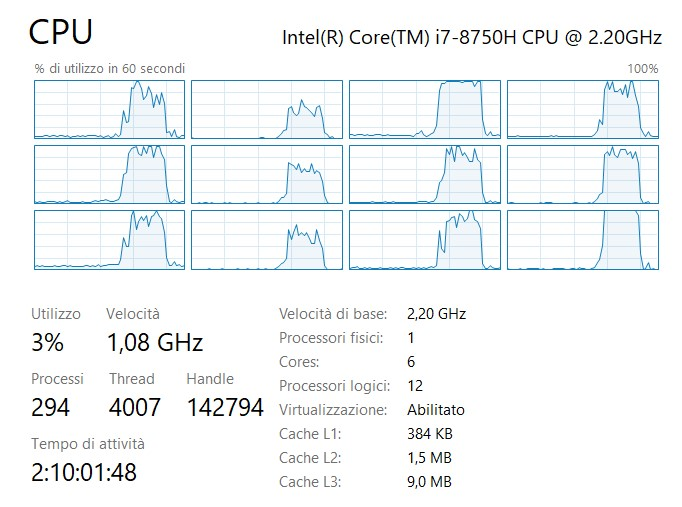
\includegraphics{images/parallel_computing.jpg}
\caption{\label{fig:cpumonitor}local machine monitoring of cores during parallel scraping}
\end{figure}

\hypertarget{parallel-foreachdofuture}{%
\subsection{Parallel foreach+doFuture}\label{parallel-foreachdofuture}}

A second attempt tries to encapsulate \passthrough{\lstinline!foreach!} \citep{foreach} originally developed by Microsoft R, being a very fast loop alternative, parallelized with \passthrough{\lstinline!doFuture!}. The package registered with older back ends required rigorous effort to specify exact dependencies for child process inside foreach arguments \passthrough{\lstinline!.export!}. From a certain angle the approach could led to an indirect benefit from memory optimization. If global variables needs to be stated than the developer might be forced to focus on limiting packages exporting. Indeed since doFuture implements optimized auto dependency search this problem may be considered solved as in \citet{doFuture}. Two major looping related speed improvements may come from \passthrough{\lstinline!.inorder!} and \passthrough{\lstinline!.multicombine!} arguments which both take advantage of parallel split disorder a subsequent recombination of results. In the context where data collection order matters this is extremely wrong, but since in this case order is defined through url composition based on criteria expressed inside nodes contents this can be totally applied. A drawback of enabling .multicombine is a worst debugging experience since errors are thrown at the end when results are reunited and no traceback of the error is given.

The upper part in \ref{fig:foreachdofuture} displays lower initialization lag from R sessions opening and parallel execution that also lead to a lower mean execution time of 6.42 seconds. No other interesting behavior are detected.
The lower plot displays high similarities with the curves in \ref{fig:furrrfuture} highlighting an outlier in the same proximities of 45/50 urls. The blue simulation repetition shows an uncommon pattern that is not seen in the other plot. Segmented variability from 40 to 80 suggests a higher value which may be addressed do instability. As a result the approach is discarded in favor of furrr + future which also offers both a comfortable \{Tidyverse\} oriented framework and offers and easy debugging experience.

\begin{figure}
\centering
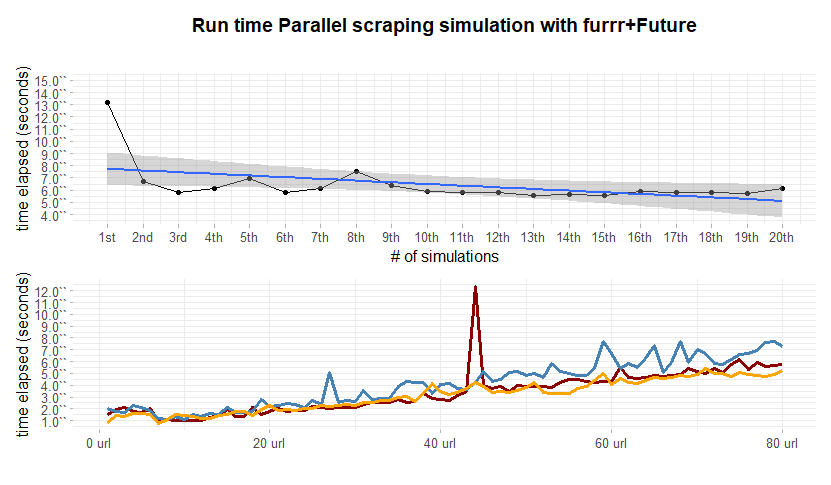
\includegraphics{images/simulations/final_foreach_dofuture.png}
\caption{\label{fig:foreachdofuture}computational complexity analysis with Furrr}
\end{figure}

\hypertarget{legal}{%
\section{Legal Profiles}\label{legal}}

There is a legitimate \emph{gray} web scrapers area, not only creating possible new uses for the data collected, but also potentially damaging the host website \citep{WhatCour57}. Online platforms and the hunger for new data insights are increasingly seeking to defend their information from web scrapers. Online platforms are unfortunately not always successful distinguishing users between polite, impolite and criminals, risking new ones valid competition and creativity. A minimal but effective self limitation can really be satisfactory for both of the parts.
In fact courts have fought hard to achieve clear judgments cases for web scraping. The crucial obstacle is a coherent verdicts to ascertain ``Kitchen Sink'' \citep{zamora2019making}, the standard web claim discontroversy on scraping. Kitchen Sink main arguments are:

\begin{itemize}
\tightlist
\item
  Legal lawsuits under the Computer Fraud and Abuse Act (CFAA) allegation that the defendant ``overtook'' allowed access \citep{UnitedSt65}
\item
  Copyright infringement charges under the Digital Millennium Act or federal copyright law Copyright laws \citep{AuthorsG59}
\item
  ``state trespass to chattels claims'' \citep{Register77}
\item
  Contract agreements terms violation claims \citeyearpar{Register77}
\end{itemize}

A second challenge to clear verdicts is that there are several purposes for which a business model operates in a continuum of social acceptability hiring web scrapers \citep{ADetaile90}. As an example Googlebot ranks, sorts and indexes search results for Google users, without which the search would not optimized and business would not profit from this fact. A more coherent case is represented by the exploitation of scraping on online Real Estate advertiser whose importance is ascertained by the fact that they are the fist house purchase media 52\% (USA survey) and searches are expected to be growing by 22\% per yeay \citep{peterson2003consumer}. On the other hand it is estimated that the 20\% of crawlers are actually DoSsing scrapers \citep{TheInter5} causing an economic damage, as in \ref{DoS}. Unfortunately the majority of web scraping services fall between these two extremes \citeyearpar{WhatCour57}.
The most discussed and observed case regards Linkedin Corp.~``Linkedin'' vs hiQ Labs Inc.~(``hiQ'') whose claim argues the exploitation of the former personal profile data to offer a series of HR services. The litigation started by accusing hiQ with ``using processes to improperly, and without authorization, access and copy data from LinkedIn's website'' \citep{Letterfr71}. As reinforcement to their arguments they presented also a citation directly form their terms raising the point on copying, web scarping prohibition without their explicit consent. Furthermore Linkedin noted that technical barriers were taken into existence to restrict the access of hiQ to the platform and warned of a breach of state and federal law by ignoring such barriers \citeyearpar{WhatCour57}. As a response Hiq submitted a temporary restricting order to prevent LinkedIn from denying the access to their platform, focusing on the aspect that the motivation was led by an anticompetitive intent. Linkedin's response brought into the litigation CFAA which actually pollutes argumentation since Court evidences that CFAA is ambiguous whether it is granting or restringing the access to public available website \citep{hiQLabsI66}. In other words CFAA intent was to protect user data when they are authenticated with passwords, and in no case out of these borders. In the end the litigation moved to the Ninth Circuit where in 2019 it uphelds the preliminary injunction to prohibit LinkedIn from continuing to provide access to publicly accessible LinkedIn member profiles to the claimant hiQ Labs \citep{wiki:HiQvsLinkedIn}.

\hypertarget{Infrastructure}{%
\chapter{API Technology Stack}\label{Infrastructure}}

The previous chapter has encapsulated the main concepts behind the design of consistent, secure, and fast scraping functions with R. In truth challenges not only regard scraping per se, but also the way and how many times the service has to interact with different clients. To tell the truth, the fact that functions are compressed into scripts does not imply that are shareable and portable. As a consequence when they are executed they also need to be at first understood and secondly loaded into R, implying higher and lower dependencies, and that requires a considerably huge effort. Moreover results are actually computed, whether in parallel or not, with local machines resources that are limited in many senses. In the end files might get lost, improperly modified and security is not guaranteed.
From a restricted personal usage perspective what has been done since now is totally feasible. But in a large-scale orientation where different stakeholders should gather massive amount of data, then a unsuitable service may cause an enormous waste of time.
The following chapter tries to capture the essence and its specific context usage of each single technology involved considering the aforementioned issues. In parallel it highlights the \emph{fil rouge} that guides the chronological order according to which the stack has been developed.
The recipe proposed serves a RESTful Plumber API (an R framework) with 2 endpoints each of which calls Parallel scraping functions settled down in section \ref{scraping}. Precautions regards sanitization of users input, anti-Dossing strategies and logs monitoring. The software environment is containerized in a Docker container and \emph{Composed} with a further container housing NGINX proxy server. Orchestration of container services is managed with Docker Compose. NGINX and SSL certificates bring HTTPSecure communication restricted with authentication. An AWS free tier EC2 server hosts the orchestration of containers and the IP is made Elastic. Furthermore the software development is made automatic with a straightforward composition of cloud services that ignites sequential building when local changes are pushed to cloud repository.

Technologies involved:

\begin{itemize}
\tightlist
\item
  GitHub version control and CI
\item
  Plumber REST API, section \ref{plumberapi}
\item
  Docker containers and compose, section \ref{docker}
\item
  NGINX reverse proxy, section \ref{nginx}
\item
  HTTPS and SSL certificates \ref{HTTPS}
\item
  AWS EC2 \ref{aws}
\end{itemize}

\begin{figure}
\centering
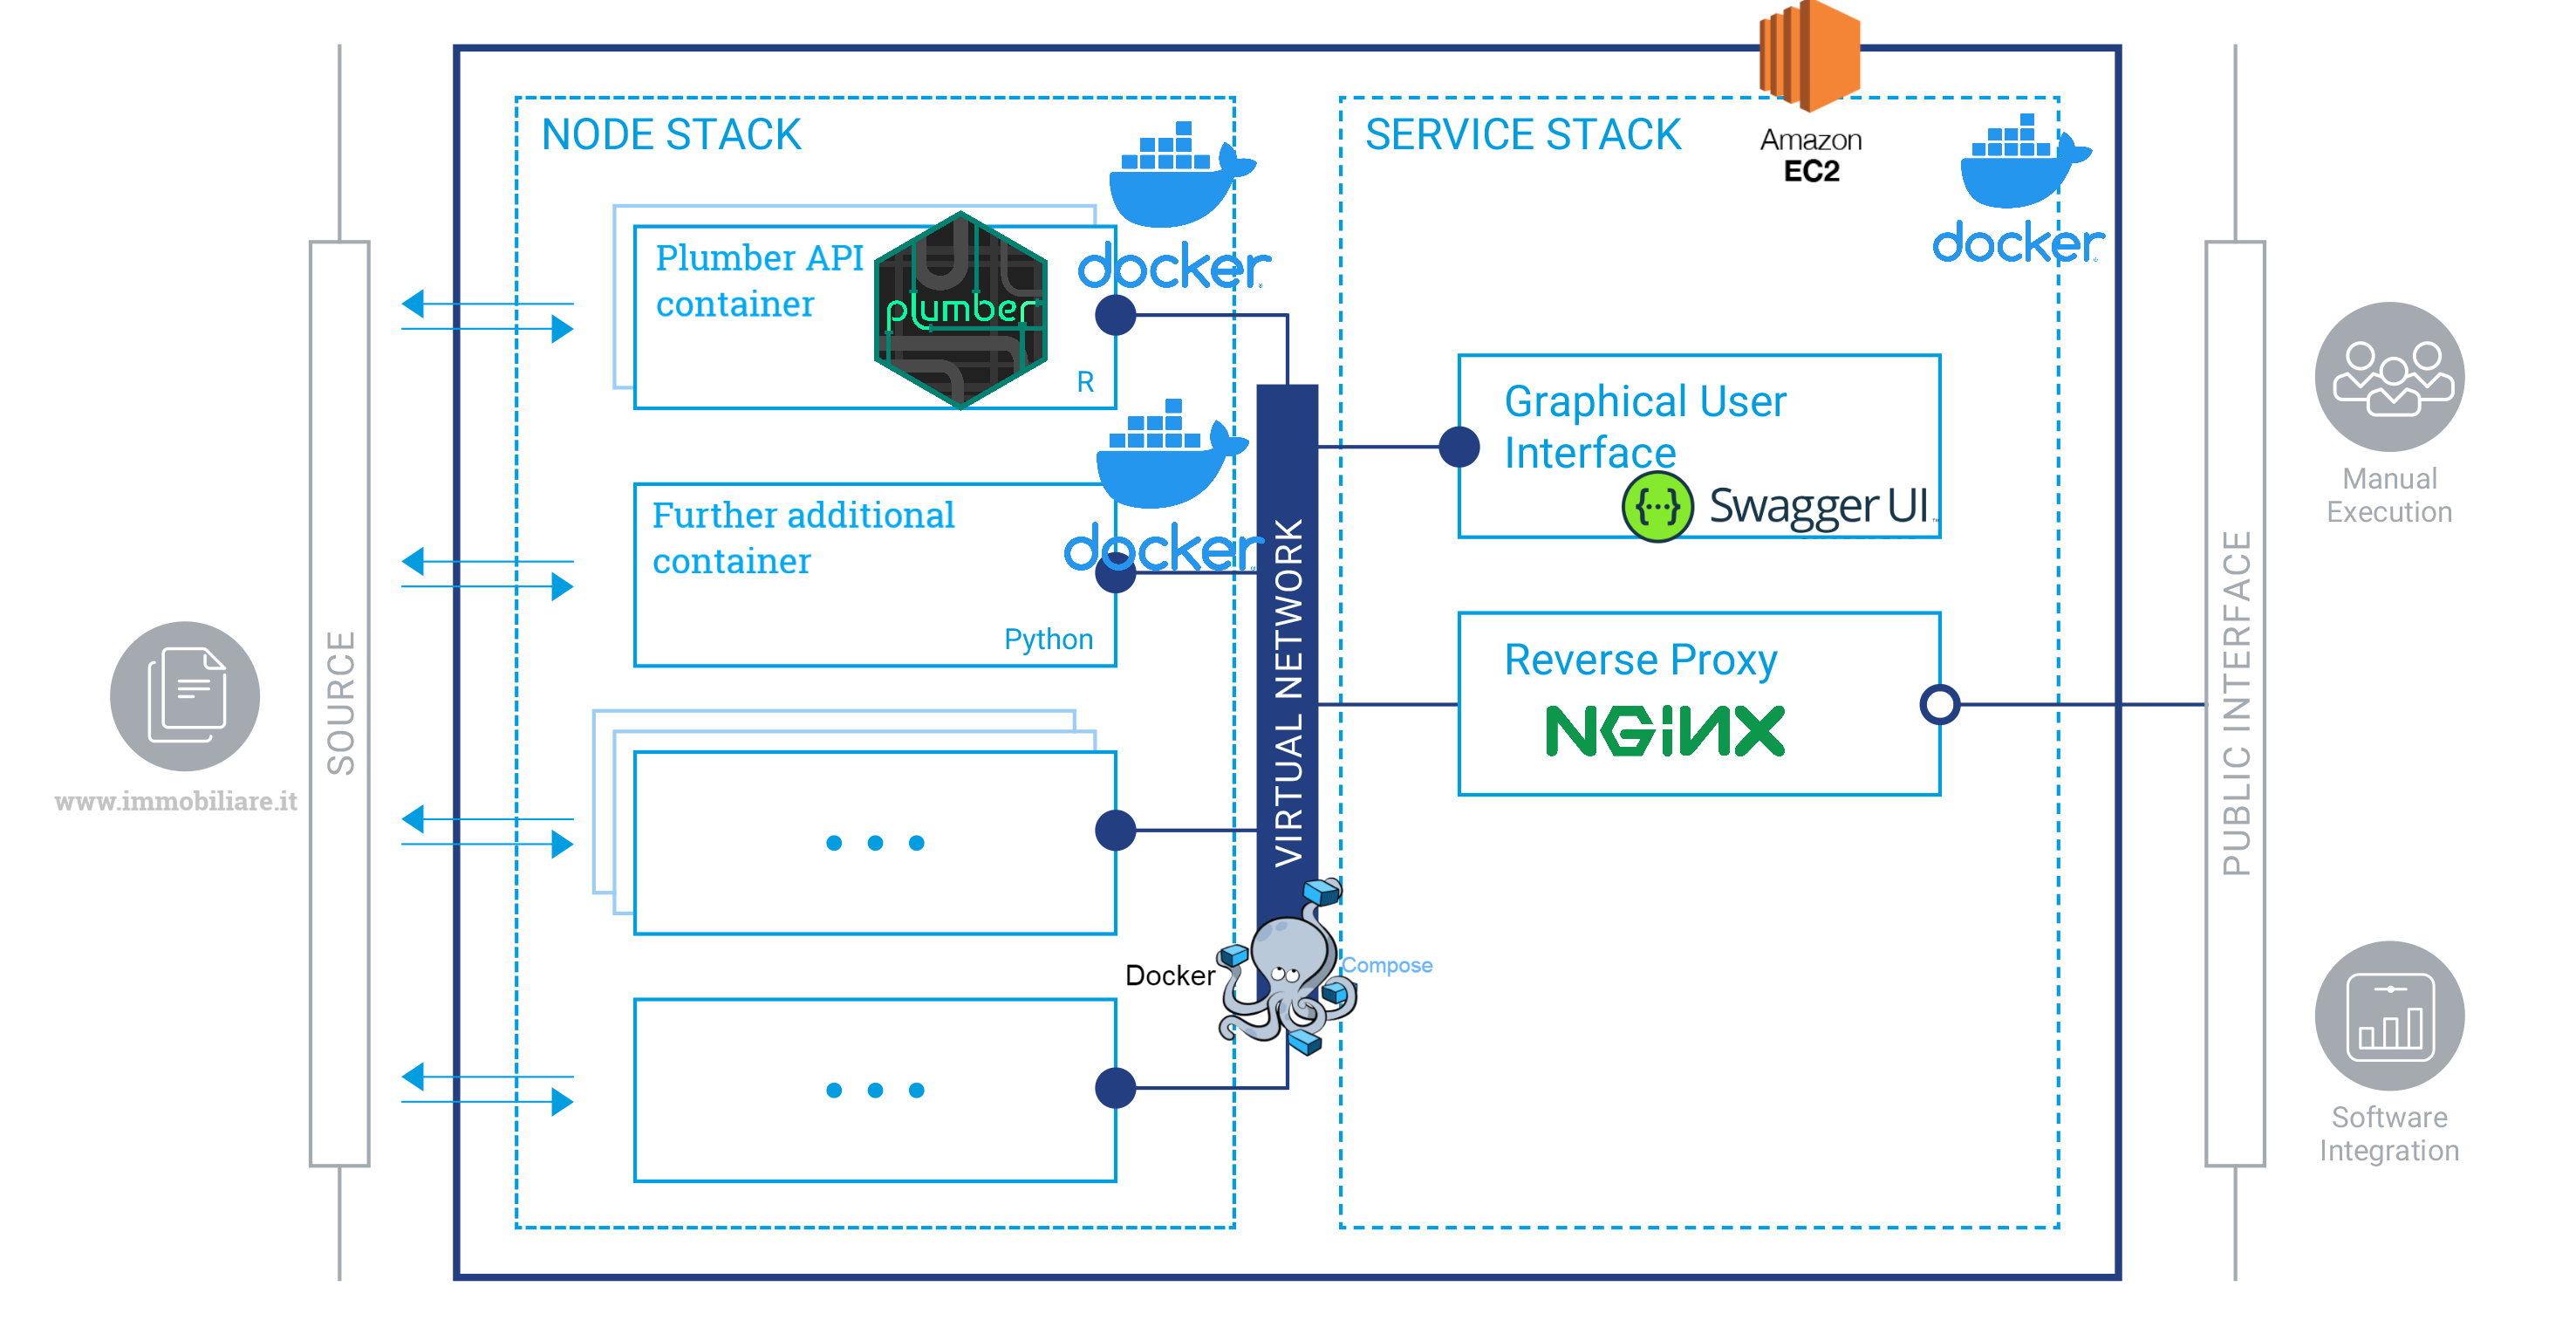
\includegraphics{images/software_arch.jpg.png}
\caption{\label{fig:CompleteStructure}complete infrastructure, author's source}
\end{figure}

As a further note each single part of this thesis is oriented to the service inspiring criteria of portability and containerization. RMarkdown \citep{rmarkdown1} documents (book's chapters) are knitted (i.e.~compiled) and then rendered as .html files through Bookdown \citep{bookdown2}. The resulting .html documents are instructed by a .yml file which suggests general settings and layout, then are condensed in a Gitbook format. Gitbooks are interactive online documentation that are employed to build books, technical documentation as well as research papers. Since documents are html files widgets are available making the dissertation responsive. Moreover Gitbooks format enables UI buttons to either create a push requests, (suitable for reviewing) or directly share publication on social media. Gitbooks are highly flexible in terms of style, up to the limit of css allowing to do so.
Rendered files are ultimately pushed to a \href{https://github.com/NiccoloSalvini/thesis}{Github repository} bringing thesis' version control. By a simple trick with GH pages a new branch is opened. .html files are displayed into a sub domain repository hosted at \citep{link}(\url{https://niccolosalvini.github.io/thesis/}). Furthermore the Gitbook is also able to produce a .pdf version output through a Xelatex engine. Xelatex compiles .Rmd documents according to formatting rules contained in a further .ylm file and a default .tex template. By doing that the .pdf output is rendered.

\hypertarget{restful-api}{%
\section{RESTful API}\label{restful-api}}

\begin{definition}[API]
\protect\hypertarget{def:api}{}{\label{def:api} \iffalse (API) \fi{} }API stands for application programming interface and it is a set of definitions and protocols for building and integrating application software. Most importantly APIs let a product or a service communicate with other products and services without having to know how they're implemented.
\end{definition}
API may be considered as a mediator between users or clients sending a request, left part figure \ref{fig:apigenstru} and the web resource or services they want (returning back a response) middle part figure \ref{fig:apigenstru}. It also acts as means of exchanging resources and knowledge with an entity, as databases left part figure \ref{fig:apigenstru} preserving protection, control and authentication, such as who gets access to what.
There are many types of APIs that exploit different media and architectures to communicate with apps or services.
\begin{definition}[REST]
\protect\hypertarget{def:rest}{}{\label{def:rest} \iffalse (REST) \fi{} }The specification REST stands for \textbf{RE}presentational \textbf{S}tate \textbf{T}ransfer and is a set of \emph{architectural principles}.
\end{definition}

If a client request is made using a REST API, a representation of the resource state is passed to a requestor or \emph{endpoint} \citep{what_is_a_rest_api}. This information is returned in one of the formats of multiple formats using \emph{HTTP}: JSON, HTML, XLT, Python, PHP or simple text. JSON is the most common programming language to use because it is language agnostic \citeyearpar{what_is_a_rest_api} and easy to interpretable both for people and machines.
REST architecture depends upon HTTP, as a matter of fact REST API inherits from HTTP the stateless property, second pillar in \ref{HTTPmethod}. Calling a REST API (producing a request) demands composing a well defined URL lower part in figure \ref{fig:apigenstru}, whose semantic is able to uniquely identify the resource or a group of resources (sending back a response) along with the most common HTTP methods, as GET, PUT, POST, DELETE.

\begin{figure}
\centering
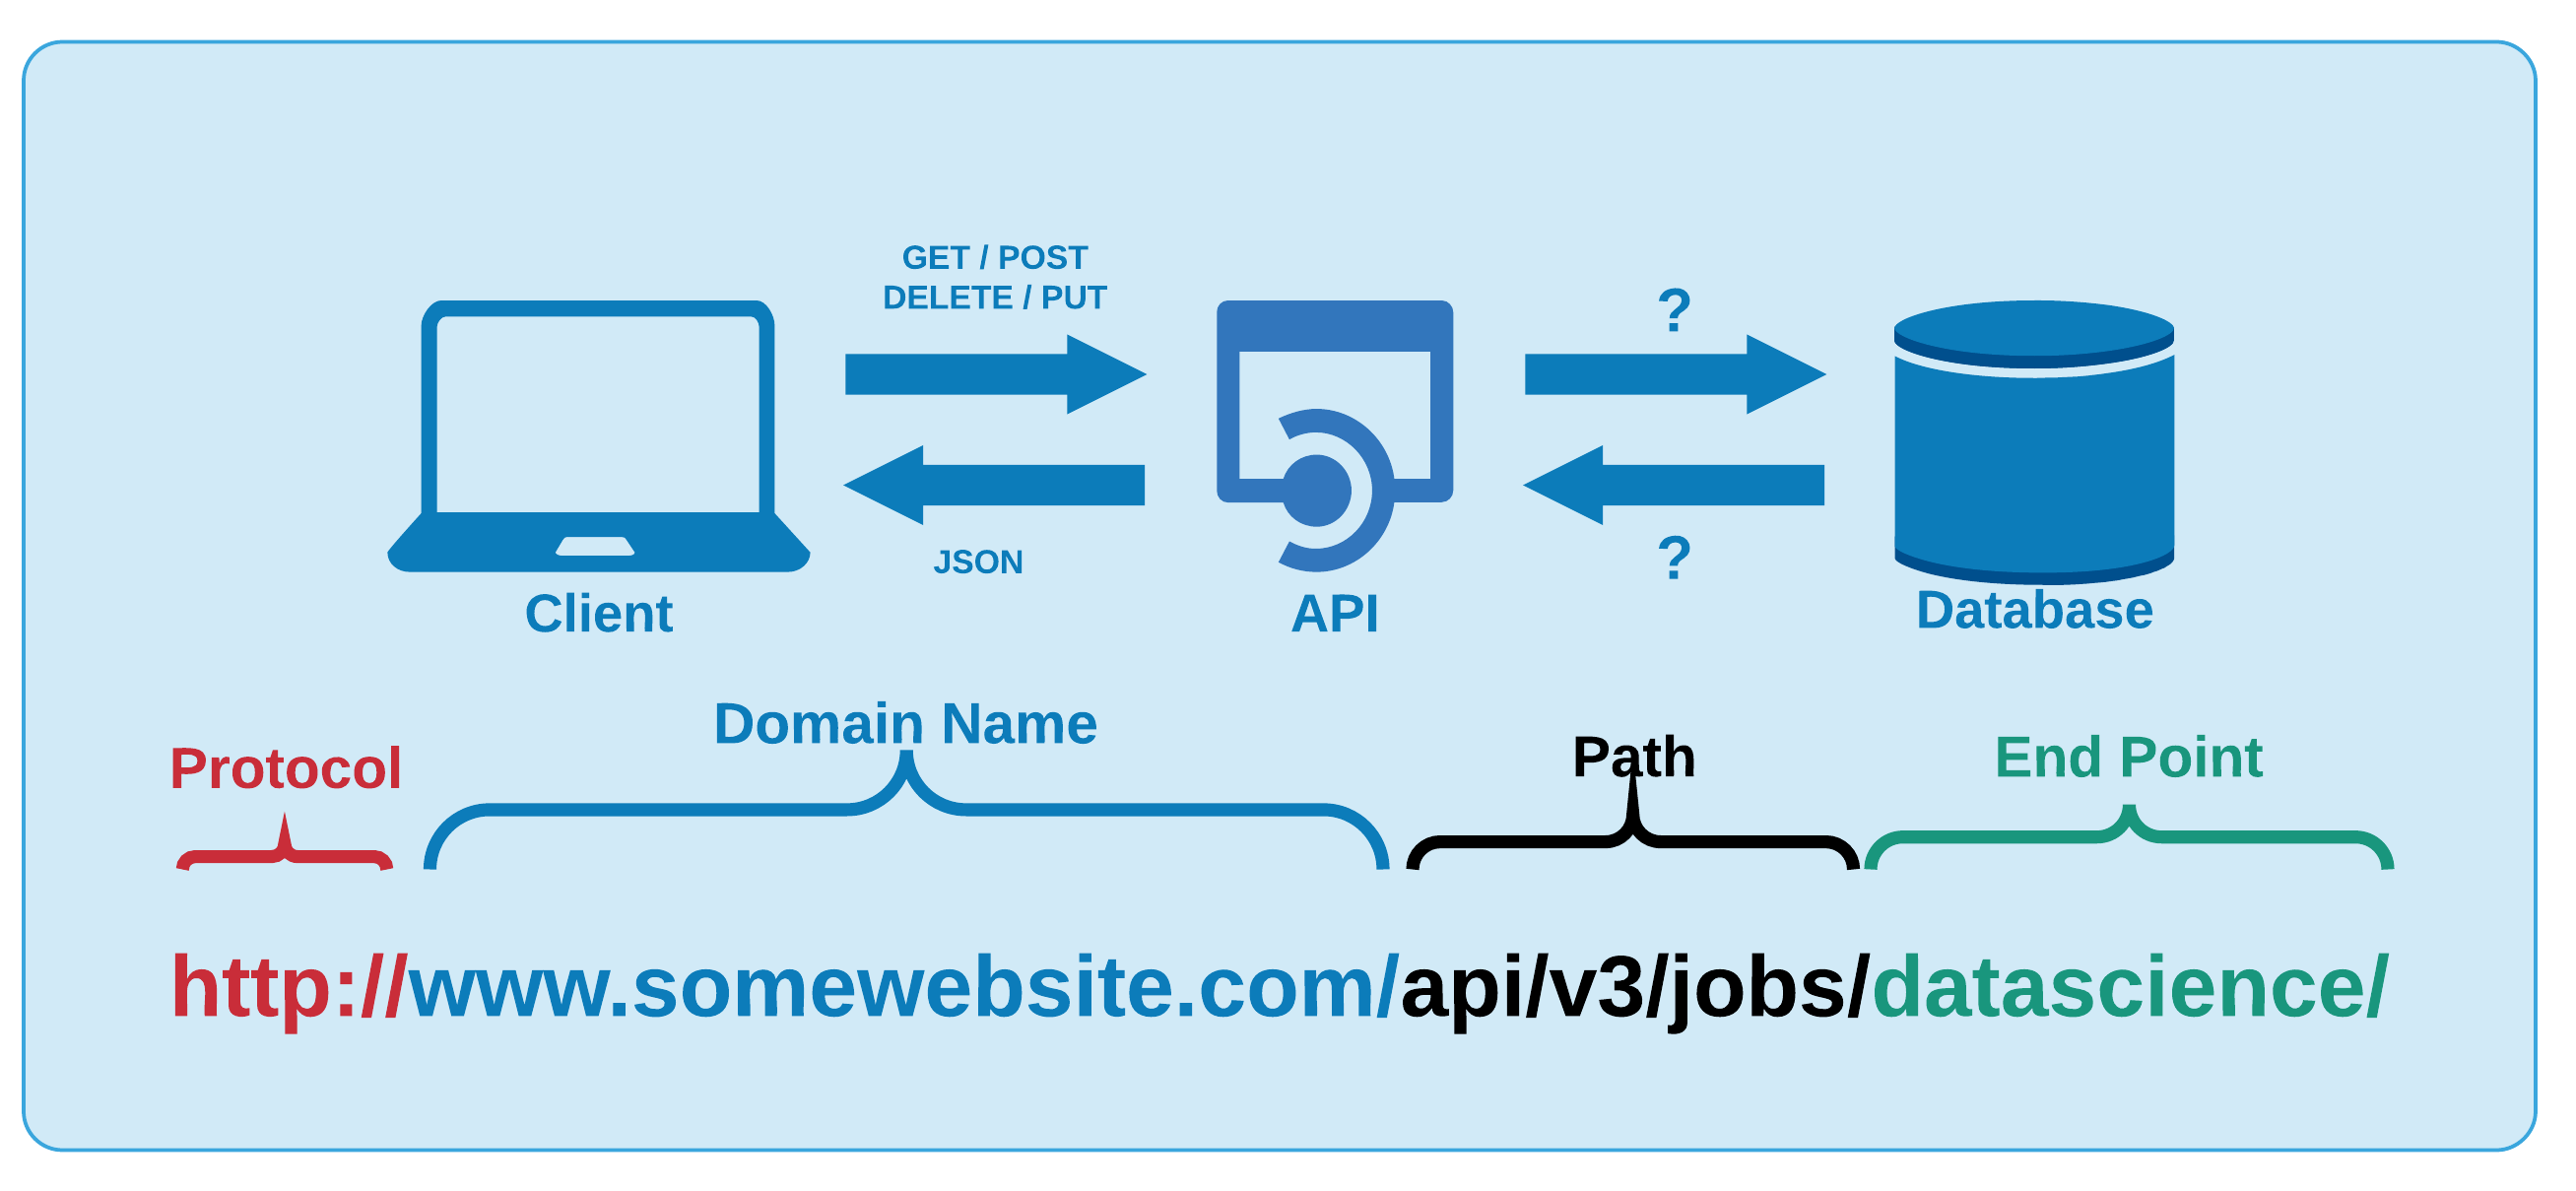
\includegraphics{images/api_stru.png}
\caption{\label{fig:apigenstru}API general functioning, unknown source}
\end{figure}

When an API adheres to REST \ref{def:rest} principles is said RESTful. Principles are:

\begin{itemize}
\tightlist
\item
  A client-server architecture made up of clients, servers, and resources, with requests managed through HTTP method.
\item
  Stateless client-server communication, meaning no client information is stored between requests and each request is separate and disconnected.
\item
  Cacheable data that streamlines client-server interactions.
\item
  A uniform interface between components so that information is transferred in a standard form. This requires that:

  \begin{itemize}
  \tightlist
  \item
    resources requested are identifiable and separate from the representations sent to the client.
  \item
    resources can be manipulated by the client via the representation they receive because the representation contains enough information to do so.
  \item
    self-descriptive messages returned to the client have enough information to describe how the client should process it.
  \end{itemize}
\item
  A layered system that organizes each type of server (those responsible for security, load-balancing, etc.) involved the retrieval of requested information into hierarchies, invisible to the client.
\end{itemize}

RESTful APIs receives HTTP request inputs and elaborates them through endpoints. Endpoints are the final step in the process of submitting an API request and they can interpreted as the responsibles for generating a response \citeyearpar{plumber}. Further documentation and differences between HTTP and REST API are beyond the scope, indeed a summary can be found to this \href{https://docs.aws.amazon.com/it_it/apigateway/latest/developerguide/http-api-vs-rest.html}{link}.
Open and popular RESTful API examples are:

\begin{itemize}
\tightlist
\item
  BigQuery API: A data platform for customers to create, manage, share and query data.
\item
  YouTube Data API v3: The YouTube Data API v3 is an API that provides access to YouTube data, such as videos, playlists, and channels.
\item
  Skyscanner Flight Search API: The Skyscanner API lets you search for flights \& get flight prices from Skyscanner's database of prices, as well as get live quotes directly from ticketing agencies.
\item
  Openweathermap API: current weather data for any location on Earth including over 200,000 cities.
\end{itemize}

\hypertarget{plumberapi}{%
\subsection{Plumber HTTP API}\label{plumberapi}}

Plumber is a R framework \citep{plumber}, allowing users to construct HTTP APIs simply by adding decoration comment to the existing R code, in this context to scraping code. Decorations are a special type of comments that suggests to Plumber where and when the API specifications start. Below is reported a toy API with 3 endpoints inspired by the original documentation. Endpoints in the following code chunk are identifiable by the three distinguishing comment blocks, separated by the aforementioned decorations. http API specifications require the user to set the endpoint description (first comment), to specify the parameters role and input type (second), and the http method i.e.~GET, POST followed by the endpoints invokation verb e.g.~echo, plot, sum (third).

Once HTTP api calls are sent to machines belonging to a single server or a network of servers, whether it is public or private they converge through endpoints. Endpoints execute functions involving the parameters specified through the call and by default response is JSON type. The first endpoint ``echo'' invocation simply \emph{echoes} back the text that it was sent. The second endpoints generates a histogram \emph{plot} i.e.~.png file based on a Normally distributed sample whose observation number are ``n''. The third endpoint calculates the \emph{sum} of a couple of number attached to the call. Scraping function are then implemented within the API framework and arguments becomes parameters for an incoming request. Many more options may induce plumber endpoints to respond in the preferred fashion, in any case are beyond the scope of the analysis.
Exposing APIs on a private network or on a public server security is a major issue. Concerns and thought process therefore must adapt accordingly. There are several variables and consequent attacks that should be considered while creating Plumber APIs, but the focus will differ depending on the API audience. For example if APIs are offered without authentication on the Internet, potential vulnerabilities should seriously convince the api maintainer to properly account each of them. Three in the context of the analysis are critical:

\begin{itemize}
\tightlist
\item
  Sanitization
\item
  Denial Of Service (DoS)
\item
  Logging
\end{itemize}

\hypertarget{sanitize}{%
\subsection{Sanitization}\label{sanitize}}

Whenever APIs accept input from a random user this is directly injected into functions through endpoints, therefore the worst case scenario should be prepared. In the context of the analysis users are required to specify to the endpoints arguments such as cities, zones, number of pages and many others. Chances are that users might either misspell inputs or use different encoding (accents) or rather use capital letters when functions are capital sensitive. Endpoints should take account of the behavior by sanitizing whatever it comes into the function. The process at first requires an intense and creative investigation on what it can be misused and how. Then Secondly new functional inputs are defined so that they take the user generated input and give back a sanitized version inside the function. In the code chunk below are shown a couple of examples of sanitization of inputs:

\begin{lstlisting}[language=R]
tipo = tolower(type) %>% str_trim()
citta = tolower(city) %>% iconv(to = "ASCII//TRANSLIT") %>% str_trim()
macroozone = tolower(macrozone) %>% iconv(to = "ASCII//TRANSLIT") %>% str_trim()
\end{lstlisting}

Inputs make their entrance into functions through arguments ``type'', ``city'' and ``macrozone'' and are immediately preprocessed. They are in sequence converted to lower cases, then extra spaces are trimmed, in the end accents are flattened.

\hypertarget{DoS}{%
\subsection{Denial Of Service (DoS)}\label{DoS}}

Denial-of-service attacks (DoS) are used to temporarily shut down a server or service through traffic congestion. A DoS scenario could be triggered accidentally by a malicious user requesting the server for an infinite looping task. Other scenarios might depict a malicious hacker who uses a large number of machines to repeatedly make time consuming requests to occupy the server, this is the case of DDoS (Distributed Denial of Service). DoS or DDoS attacks may also induce anomalies and deprives system resources, which in the context of hosting services may result in astronomical fees charged. Dos attack as a conseuquence may also induce distorted website/API logs analytics, leading to distorted reports.
A simple but effective approach tries to limit and stop the number of request sent:

\begin{lstlisting}[language=R]
 if (npages > 300 & npages > 0){
                        msg = "Don't DoS me!"
                        res$status = 500 # code num: Bad request
                        stop(list(error=jsonlite::unbox(msg)))     
            }
\end{lstlisting}

The code chunk above intercepts DoS attacks by limiting to 300 the number of pages to be server to the API. Furthermore it converts outputs error messages printed on console into JSON format and then pass them as output. This simplify distinguishing malicious attacks from a type errors. DDoS attacks are secured by SSL certificates and Authentication covered later in the chapter.

\hypertarget{logging}{%
\subsection{Logging}\label{logging}}

Plumber uses ``filters'' that can be resorted to describe a ``pipeline'' for processing incoming request. This enables API maintainers to separate complex logic into discrete, comprehensible steps. Usually, before trying to find an endpoint that satisfies a request, Plumber passes the request through the \emph{filters}. When APIs are called, requests pass through filters one at a time and Plumber forwards i.e.~\passthrough{\lstinline!forward()!} the request to the next filter untill the endpoints. Filters applications ranges from excluding client request based on request parameters or may offer also a thin layer of authentication. Filters might also be used as a logging for requests where logging, i.e.~the act of keeping a log {[}@{]}, is recording events in an operating system or running software from other users of communication software, or messages among different subjects.
A request log filter might have this appearance:

\begin{lstlisting}[language=R]
#* Log information
#* @filter logging
function(req){
            cat(as.character(Sys.time()), "-",
                req$HTTP_USER_AGENT, "@", 
                req$REMOTE_ADDR, "\n",
                req$QUERY_STRING, "\n")
            plumber::forward()
}
\end{lstlisting}

The above filter parses the request through the default request argument \passthrough{\lstinline!req!}, then it prints out messages about the incoming User Agent (i.e.~\passthrough{\lstinline!HTTP\_USER\_AGENT!}) (section \ref{spoofing}), the \passthrough{\lstinline!REMOTE\_ADDR!} which is the IP address of the client making the request \citeyearpar{plumber} and the \passthrough{\lstinline!QUERY\_STRING!} that records the parameters directly sent the endpoint. This helps to traceback clients activity on the API as well as detecting misuse.

\hypertarget{docs}{%
\subsection{RESTful API docs}\label{docs}}

The service disposes of 2 endpoints \emph{/fastscrape} , \emph{/completescrape}. Parameters, aligned next to the endpoint name in figure \ref{fig:swagger}, are the same for both of the endpoints since they rely on the same reverse engineering url algorithm \ref{fig:pseudocode3}, exaplined in section \ref{reverse}. Moreover Plumber APIs are natively wrapped up around Swagger UI helping development team or end users to imagine and communicate with the resources of the API without any discharge logic \citep{swaggerUI}. The OpenAPI (formerly referred to as Swagger), with the visual documentation facilitates backend implementation and client side consumption, as well as being automatically created by the APIs specification (parameters, endpoints\ldots). Some of the major assets in Swagger UI are: The user interface works in any environment, whether locally or web and it is suited for all main browsers.
Rest API documentation can be reached to the API address in the \passthrough{\lstinline!/\_\_docs\_\_/!} path, in the upper navigation bar of figure \ref{fig:swagger}. A further parameter argument, namely \passthrough{\lstinline!thesis!} into both of the endpoint has been added in order to make the API calls reproducible by providing to the scarping function a pre-compiled url to scrape.

\begin{figure}
\centering
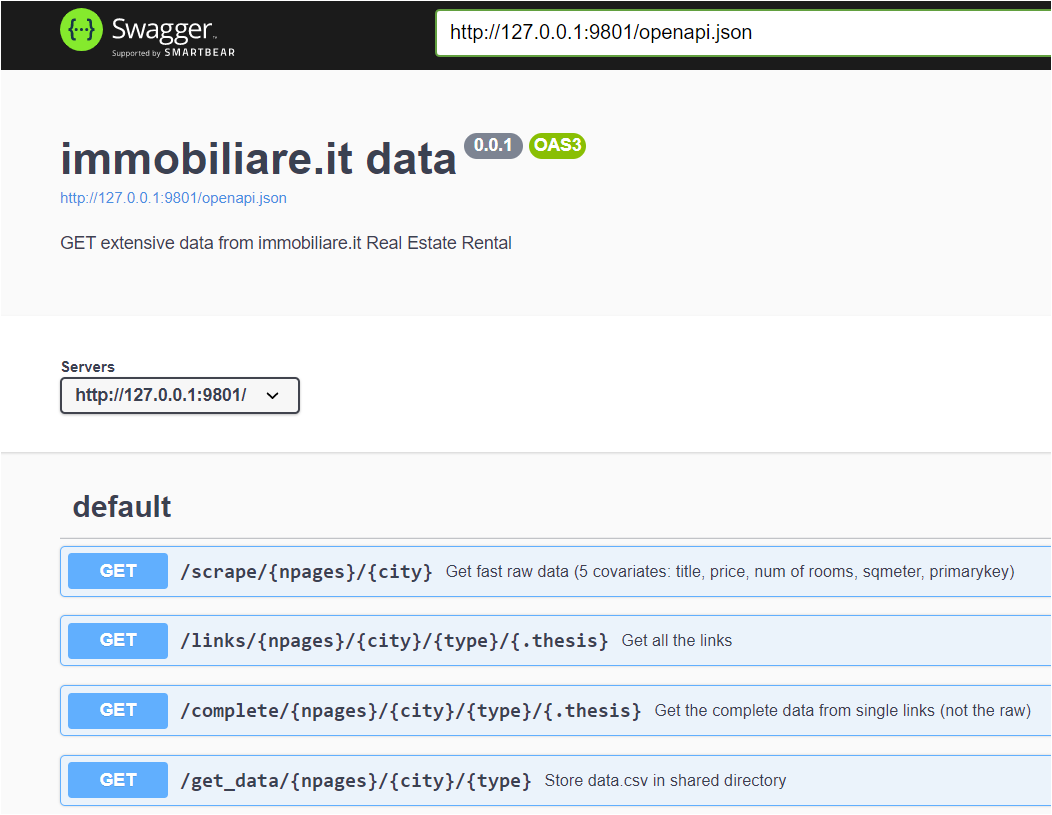
\includegraphics{images/swagger.PNG}
\caption{\label{fig:swagger}Swagger UI in localhost on port 8000, author's source}
\end{figure}

An API call might look like the following for both of the endpoint, further details (apart from the minimal requirements in the Swagger UI) are found in the api documentation at the GitHub repository \citet{NiccoloS11}.

\begin{figure}
\centering
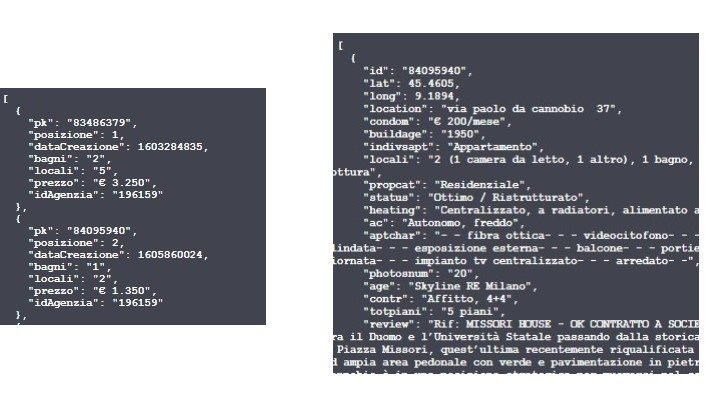
\includegraphics{images/endpoint1and2.jpg}
\caption{\label{fig:endpoint1and2}Left: API fastscrape endpoint JSON results, Right: API completescrape endpoint JSON results author's source}
\end{figure}

\hypertarget{docker}{%
\section{Docker}\label{docker}}

The API up to this point needs a dedicated lightweight software environment that minimizes dependencies both improving performances and enabling \emph{cloud computing} coverage. A fast growing technology known as \emph{Docker} might extend these capabilities.
\begin{definition}[Docker and Containers]
\protect\hypertarget{def:docker}{}{\label{def:docker} \iffalse (Docker and Containers) \fi{} }\emph{Docker} \citep{docker} is a software technology to create and deploy applications using containers.
\emph{Docker containers} are a standard unit of software (i.e.~software boxes) where everything needed for applications, such as libraries or dependencies can be run reliably and quickly. Containers are also portable, in the sense that they can be taken from one computing environment to the following without further adaptations.
\end{definition}
Containers can be thought as a software abstraction that groups code and dependencies together. One critical advantage of containers is that multiple containers can run on the same machine with the same OS along with their specific dependencies (docker compose). Each container can run its own isolated process in the user space, so that each task/application is exhaustively and complementary to the other. The fact that containers are treated singularly enables a collaborative framework that it also simplifies bugs isolation.

Actually \emph{Docker containers} are the build stage of \emph{Docker Images}. Docker images therefore are the starting point to containerize a software environment. They are built up from a series of software layers each of which represents an instruction in the image's \emph{Dockerfile} \citeyearpar{docker_documentation_2020} . In addition images can be open sourced and reused through Docker Hub.
\emph{Docker Hub} is a web service provided by Docker for searching and sharing container images with other teams or developers in the community. Docker Hub can authorize third party applications as GitHub entailing an collaborative image version control, this would be critical for software development as disguised in section (\ref{sdwf}).

\hypertarget{dockerfile}{%
\subsection{REST-API container}\label{dockerfile}}

Docker can build containers from images by reading instructions from a Dockerfile. A Dockerfile is a text document that contains the commands/rules a generic user could call on the CLI to assemble an image. Executing the command \passthrough{\lstinline!docker build!} from working directory the user can trigger the build. Building consists of executing sequentially several command-line instructions that specifies the software environment. As a matter of fact the concept of containers takes inspiration by the fact that many single software layers are stacked up over at the following. An open source project named \href{https://www.rocker-project.org/images/}{rocker} already disposes of a group of pre-set task-specific image configurations from which further custom dockerfile can be built on top of.
Therefore images are overwritten with higher level dependencies i.e.~package libraries, since lower levels Linux dependencies are already partially handled. Indeed as in \ref{sdwf} an automatic development workflow is proposed that triggers the building of the image when changes are pushed to github.

The custom Dockerfile in figure \ref{fig:dockerfile}) is able to build the rest-api container:

\begin{figure}
\centering
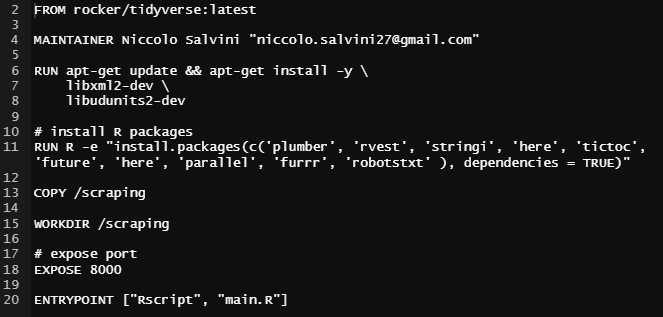
\includegraphics{images/dockerfile2.PNG.jpg}
\caption{\label{fig:dockerfile}Custom Dockerfile from salvini/api-immobiliare Docker Hub repository, author's source}
\end{figure}

Each line from the Dockerfile has its own specific role:

\begin{itemize}
\item
  \passthrough{\lstinline!FROM rocker/tidyverse:latest!} : The command imports from rocker project a pre set config guration containing the latest version of base-R along with the tidyverse \citep{tidyverse} R packages collection.
\item
  \passthrough{\lstinline!MAINTAINER Niccolo Salvini "niccolo.salvini27@gmail.com"!} : The command tags the maintainer and its e-mail contact information.
\item
  \passthrough{\lstinline!RUN apt-get update \&\& apt-get install -y \\ libxml2-dev \\ libudunits2-dev!} : The command update and install remaining OS Linux dependencies required to run Plumber and rvest.
\item
  \passthrough{\lstinline!RUN R -e "install.packages(c('tictoc','here','...',dependencies=TRUE)!} : The command install all the further lower level libraries required to execute the files. Since some packages have inner dependencies the option \passthrough{\lstinline!dependencies=TRUE!} is necessary.
\item
  \passthrough{\lstinline!COPY /scraping!} : The command tells Docker to copy into the container files in /scraping folder (where API specs are)
\item
  \passthrough{\lstinline!WORKDIR /scraping!} : The command tells Docker to set /scraping as working directory
\item
  \passthrough{\lstinline!EXPOSE 8000!} : The commands instructs Docker engine that the container listens on the specified network ports 8000 at runtime. Default \emph{transportation} layer is TCP.
\item
  \passthrough{\lstinline!ENTRYPOINT ["Rscript", "main.R"]!} : the command tells docker engine to execute the file main.R where are contained the Plumber router options (i.e.~host and port specifications).
\end{itemize}

\hypertarget{nginx}{%
\section{NGINX reverse Proxy Server and Authorization}\label{nginx}}

Proxy server in this context offers the opposite angle for the exact same security problem. As a matter of fact the downside is that they can be exploited for the same reason for which they have been criticized at the end of section (\ref{spoofing}). Reverse Proxy server are a special type of gateway \ref{def:proxy} that is usually located behind a private network firewall to route client requests to the corresponding backend server \citep{nginxDocs}. An reverse proxy offers an extra abstraction and control level to ensure that network traffic flows smoothly between clients and servers. NGINX as it can be inferred by its official documentation empowers traffic flows by:

\begin{itemize}
\item
  \emph{Load balancing}: A reverse proxy server will stand guard in front of back end servers and redirect requests across a group of servers in a way that maximizes speed and capacity usage as well as not overloading the server. When a server crashes, the load balancer redirects traffic to the other online servers (note required since traffic is not expected to be enormous).
\item
  \emph{Web acceleration}: A reverse proxies can condense input and output data by caching frequently requested information. This assists traffic between clients and servers avoiding to request data more than once. They can also apply SSL encryption, which improves their performance by eliminating loads form web servers.
\item
  \emph{Security and anonymity}: A reverse proxy server protects identities and serves as an additional protection against security threats seen in sub-sections (\ref{sanitize}, \ref{Dos}) by intercepting requests before they reach end server.
\end{itemize}

When a user calls the API, NGINX acts as a gateway asking for credentials and registering log data (HTTP identification headers). If the request has already been asked then cached response is returned. If it does not then the request is routed to the endpoint, service A and B in figure \ref{fig:nginxfun}. Endpoints elaborate the request into the response, which flows back at first to the gateway and then finally to the client. Logging data can be feeded to a dashboard monitoring traffic and API exposure.

\begin{figure}
\centering
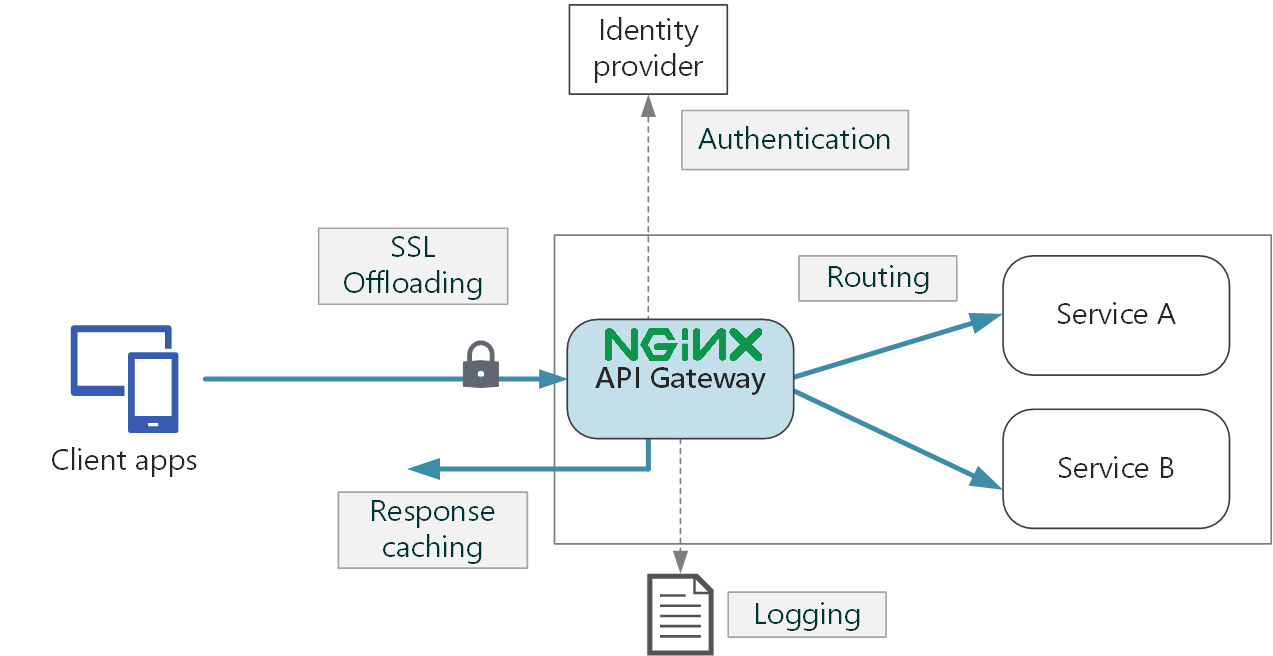
\includegraphics{images/nginx_gateway.png}
\caption{\label{fig:nginxfun}NGINX gateway redirecting an incoming request, source \citet{azureNGINX}}
\end{figure}

Then without any further software installation, the developer can simply make use of the latest NGINX open sourced image to build the NGINX proxy server within the same image. A further configuration file should manage NGINX inner settings that links volumes, ports and IPs, but details are beyond the scope of the analysis.

\hypertarget{docker-compose}{%
\section{Docker-Compose}\label{docker-compose}}

Compose is a multi-container Docker framework to define and run complex application and services, that means isolated stand alone containers can communicate one to each other. The orchestration of containers is managed through a .yaml file docker-compose.yml that configures the whole set of facilities designed for the services. Services are then build with a single docker command \passthrough{\lstinline!docker-compose up!} on the basis of the instruction yaml file. Compose also enables \emph{Volumes}, which are used in Docker for \textbf{data persistence} \citep{dockervolumes}. VOlumes allows to keep data secured from docker stop or delete containers. Docker Volumes ina nutshell works as the linkage between a physical file system path (folders, directories) plugged/\textbf{mounted} into the virtual container file system path.
The main properties for Composition as in documentation \citep{docker_documentation_2020} regards:

\begin{itemize}
\tightlist
\item
  \emph{A central host in multiple isolated environments}: Compose provides a label for a project to distinguish environments. The default project name is the directory path.
\item
  \emph{Preserve data volumes (which are the preferred Docker mechanism to consume data generated and used by containers) when building containers}: Compose maintains all of the services' Volumes. When Docker-compose is running, it transfers the Volumes from the old container into the new container when it detects containers from previous runs. This method guarantees that no Volume data produced is lost.
\item
  \emph{Only recreate containers that have changed}: Compose caches the configuration and re-use the same containers when it reboot a service which hasn't changed. Re-use containers means it provides really fast improvements to the environment when developing complex services.
\item
  \emph{Variables and moving a composition between environments}: Compose supports file variables which might be used to adjust any composition to various environments or users.
\end{itemize}

\begin{figure}
\centering
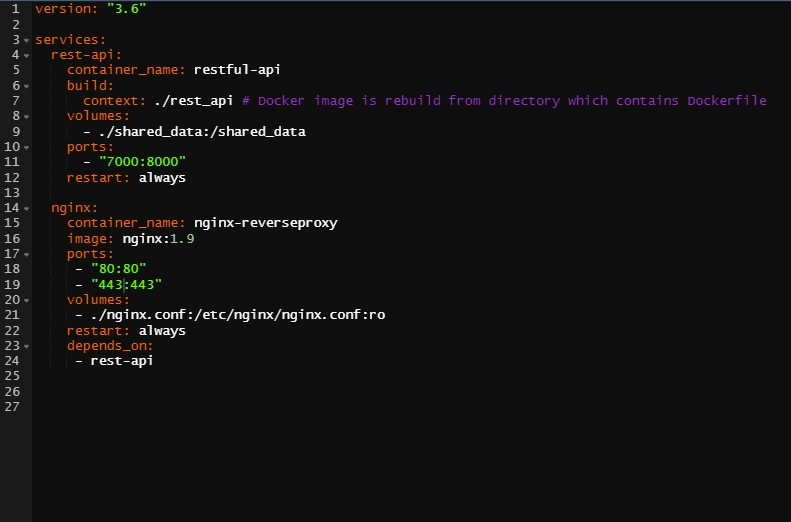
\includegraphics{images/docker-compose.jpg}
\caption{\label{fig:Compose}Docker Compose YAML file orchestration for NGINX container and RESTful API, author's source}
\end{figure}

The first line defines the versions according to which Compose orchestrates containers. Services are two, the rest-api and NGINX. The former whose name is restful-api builds the container starting from the Dockerfile contained into the rest\_api path specified as in \ref{dockerfile}. The first service also mounts Volumes from shared\_data to itself in the virtual container file path. Port 8000 opened (\ref{dockerfile}) is linked to the 7000 one. Restarting set to ``always'' secures the latest container version.
The latter service is NGINX \ref{nginx} which proxies traffic from 80 and 443 based on .conf file whose specifications are beyond the scope of the analysis. Volumes makes sure that specifications are arranged in the default path choice. The option depends\_on defines the chrono-logical condition accroding to which containers should be run and then composed.

\hypertarget{HTTPS}{%
\section{HTTPS(ecure) and SSL certificates}\label{HTTPS}}

Communication even though properly secured and distributed with NGINX is still not encrypted so sensitive data are still being exposed. HTTP Secured (HTTPS) is a product of HTTP combined with SSL/TLS (Secure Sockets Layer/Transportation Security Layer) protocol rather than a protocol itself. HTTPS is strictly appropriate when transmitting sensitive data such as banking or on-line buying. Its importance is highlighted by the fact that nowadays is rather more common to find HTTPS than HTTP. The Secured method encrypts all contacts between the client and the server, figure \ref{fig:httpsmeth}. The HTTPS scheme in actual is ``HTTPS'' and its default port is 443 (that should be exposed too in the dockerfile). SSL runs as a sublayer of the \emph{application} layer (a further internet layer, refer to section \ref{HTTPmethod}), this ensures that HTTP messages are encrypted prior being transmitted to the server (SSL Offloading box in figure \ref{fig:nginxfun}) whether it is a proxy server or directly a web server.

\begin{figure}
\centering
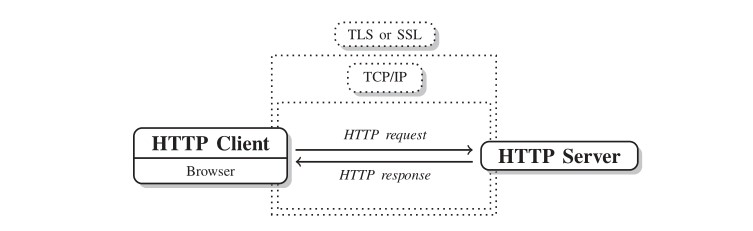
\includegraphics{images/https_method.jpg}
\caption{\label{fig:httpsmeth}HTTPS encryption with SSL certificates, source \citet{automateddatacollection}}
\end{figure}

From a port communication point of view at first NGINX container listens to on port 80 and that it is where all requests should relay to IP\_macchine\_address:8000. As a result the RESTful API is published on Port 80 instead of 8000. Secondly it listens on the SSL port 443 and points to the key and certificate files that have been created in the Dockerfile.

\hypertarget{aws}{%
\section{AWS EC2 instance}\label{aws}}

From henceforth the software container environment can be reproduced regardless of the mounted OS. Scalability and accessibility is worked out by exporting orchestrated containers on a web server. There are many hosting services options that varies primary on the budget and consequently on the API audience. A flexible cloud provider combined with NGINX load balancing \emph{ceteris paribus} may offer a stable and reliable service for a reasonable price, even considering a bad-case scenario where requests are many and insistent.
\begin{definition}[AWS EC2]
\protect\hypertarget{def:aws}{}{\label{def:aws} \iffalse (AWS EC2) \fi{} }Amazon Elastic Compute Cloud (EC2) is a web service that contributes to a secure, flexible computing capacity in the AWS cloud. EC2 allows to rent as many virtual servers as needed with customized capacity, security and storage.
\end{definition}

AWS EC2 represents a popular hosting option, most importantly this path is already narrowed by many open source contributors. The selected target is a AWS free tier t3.micro whose specifications are: 2 vCPU (Virtual CPU), 1 GB memory and a mounted Ubuntu distribution OS. Moreover T3 instances are known to provide device, memory, and network resource balance and have been developed for applications that experience transient spikes in use with modest CPU use. They are designed especially to serve low-latency interactive applications, small and medium databases, virtual desktops, development environments, code repositories, and business-critical applications, therefore they suit the needs.
Prior any new instance initialization AWS offers to tune servers' set up options. Networking and VPC are chosen to be left as is since they can always be updated at need. Storage is increased to 30 GB which represents the free tier eligibility upper limit. Indeed security at first needs to account for a SSH connection that allows communication with the server i.e.~open port 22. Secondly it should account for port openings accordingly to NGINX configuration file and rest-api dockerfile (\ref{dockerfile}), port 80 (default for TCP) and 443 (HTTPS default) are opened. Once the instance is running the server can be accessed through SSH behind authentication.

\hypertarget{sdwf}{%
\section{Software CI/CD Workflow}\label{sdwf}}

Software changes can happen quite often due to the dynamic nature of the RESTful API's target website. This requires a modern stack of cloud technologies to update, revert and quickly deploy software versions, or even integrate software architecture. As a consequence the software CI/CD manages minor changes with local commits to the project, which are then directly pushed through git to the open GitHub repository, upper left quadrant \ref{fig:sfmap}. The repository directly communicates with an DockerHub repository that sequentially triggers the compose-up command of the compose.yml file, and through that the docker images whenever any changes are pushed, upper right quadrant \ref{fig:sfmap}. Images are tagged and cached so that versions are controlled and Software build avoids to rerun containers that have not suffered any change. Debugging is constrained to logs generated by docker engine. Furthermore the build stage in R since 2019 required long time due to package compiling, but since the appearance of Rstudio \href{https://packagemanager.rstudio.com/client/\#/}{package manager} which includes beta support for pre-compiled R packages they can be installed 3 times faster \citep{nolispmanager}.
When newer images are available they can be pulled from the EC2 server and rerun in detached mode. Massive software changes are managed through GitHub branches, even though it must be kept in mind to swith lautomatic building brench. The Ec2 server is associated to an Elastic IPs address allowing to reuse the address for external databases connections and DNS services as Cloudflare (for SSL certificates). Moreover elastic IPs are effective when the EC2 server stands in need of upgrading or downgrading or when the server may fail, thus restoring and apply the IP address for a new server.

\begin{figure}
\centering
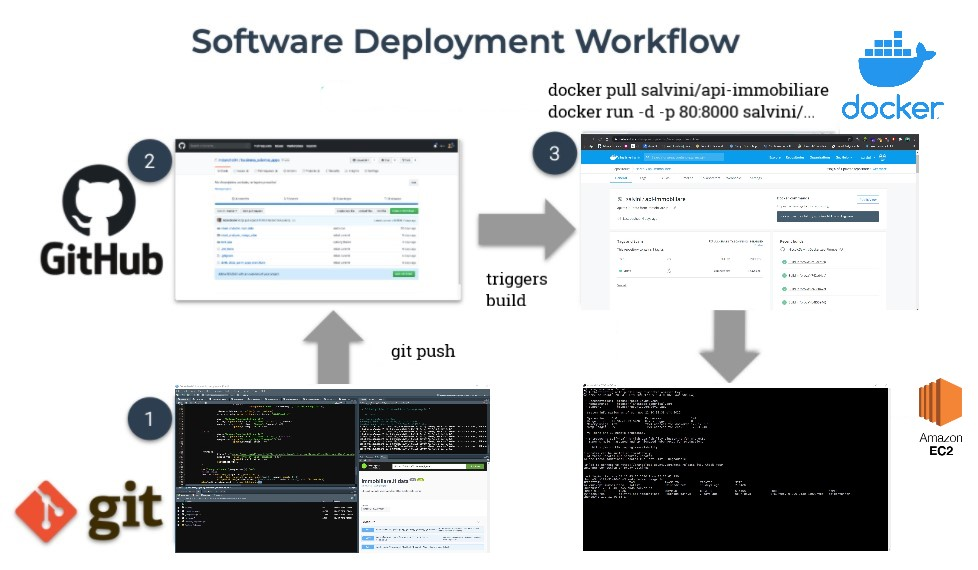
\includegraphics{images/SoftwareDevWF.jpg}
\caption{\label{fig:sfmap}Software development CI/CD workflow, author's source}
\end{figure}

\hypertarget{further-sf-integrations}{%
\section{Further SF Integrations}\label{further-sf-integrations}}

A more robust code can be obtained embedding recent R software development frameworks as \passthrough{\lstinline!Golem!} \citet{colin_fay_2020} into the existing structure, anyway this requires a complete restyle of the existing code architecture. The framework stimulates the usage of \emph{modules} to enhance reusable codes. In addition for the way it is done it forces through automatic actions, articulated into a sequence of rules to follow, to organize code and dependencies aimed at saving time to DevOps teams. It has also a labour-saving function to build custom dockerfiles based on the dependecies organized throughout the building framework.
Moreover according to the latest R-API literature, code should be veveloped as R packages as in \citet{plungr}, allowing to use inner \textbf{TDD} (i.e.Test-Driven Development \citet{TDD_2004}) mechanism with \citet{testthat} as pointed out in \citet{colin_fay_2020} section 4.2.

\hypertarget{inla}{%
\chapter{INLA}\label{inla}}

Bayesian estimation methods - by MCMC \citep{mcmc} and MC simulation techniques - are usually much harder than Frequentist calculations \citep{wang2018bayesian}. This unfortunately is also more critical for spatial and spatio-temporal model settings \citep{Cameletti2012} where matrices dimensions and densities (in the sense of prevalence of values throughout the matrix) start becoming unfeasible.
The computational aspect refers in particular to the ineffectiveness of linear algebra operations with large dense covariance matrices that in aforementioned settings scale to the order \(\mathcal{O}(n^3)\).
INLA \citep{Rue2009, Rue2017} stands for Integrated Nested Laplace Approximation and constitutes a faster and accurate deterministic algorithm whose performance in time indeed scale to the order \(\mathcal{O}(n)\). INLA is alternative and by no means substitute \citep{YT:Rue} to traditional Bayesian Inference methods. INLA focuses on Latent Gaussian Models LGM \citeyearpar{wang2018bayesian}, which are a rich class including many regressions models, as well as support for spatial and spatio-temporal.
INLA turns out to shorten model fitting time for essentially two reasons related to clever LGM model settings, such as: Gaussian Markov random field (GMRF) offering sparse matrices representation and Laplace approximation to approximate posterior marginals' integrals with proper search strategies.
In the end of the chapter it is presented the R-INLA project and the package focusing on the essential aspects.
Further notes: the chronological steps followed in the methodology presentation retraces the canonical one by \citet{Rue2009}, which according to the author's opinion is the most effective and the default one for all the related literature. The approach is more suitable and remains quite unchanged since it is top-down, which naturally fits the hierarchical framework imposed in INLA. The GMRF theory section heavily relies on \citet{GMRFRue}.\\
Notation is imported from \citet{Blangiardo-Cameletti} and integrated with \citet{Bayesian_INLA_Rubio}, whereas examples are drawn from \citet{wang2018bayesian}. Vectors and matrices are typeset in bold i.e.~\(\boldsymbol{\beta}\), so each time they occur they have to be considered such as the \emph{ensamble} of their values, whereas the notation \(\beta_{-i}\) denotes all elements in \(\boldsymbol{\beta}\) but \(\beta_{-i}\).
\(\pi(\cdot)\) is a generic notation for the density of its arguments and \(\tilde\pi(\cdot)\) has to be intended as its Laplace approximation. Furthermore Laplace Approximations mathematical details, e.g.~optimal grid strategies and integration points, are overlooked instead a quick intuition on Laplace functioning is offered in the appendix \ref{laplaceapprox}.

\hypertarget{LGM}{%
\section{The class of Latent Gaussian Models (LGM)}\label{LGM}}

Bayesian theory is straightforward, but it is not always simple to measure posterior and other quantities of interest \citep{wang2018bayesian}. There are three ways to obtain a posterior estimate: by \emph{Exact} estimation, i.e.~operating on conjugate priors, but there are relatively few conjugate priors which are also employed in simple models. By \emph{Sampling} through generating samples from the posterior distributions with MCMC methods \citep{metropolis, hastings} later applied in Bayesian statistics by \citet{gelfand1990sampling}. MCMCs have improved over time due to inner algorithm optimization as well as both hardware and software progresses, nevertheless for certain model combinations and data they either do not converge or take an unacceptable amount of time \citeyearpar{wang2018bayesian}. By \emph{Approximation} through numerical integration and INLA can count on a strategy leveraging on three elements: \emph{LGMs}, \emph{Gaussian Markov Random Fields} (GMRF) and \emph{Laplace Approximations} and this will articulates the steps according to which the arguments are treated. LGMs despite their anonymity are very flexible and they can host a wide range of models as regression, dynamic, spatial, spatio-temporal \citep{Cameletti2012}. LGMs necessitate further three interconnected elements: \textbf{Likelihood}, \textbf{Latent field} and \textbf{Priors}.
To start it can be specified a generalization of a linear predictor \(\eta_{i}\) which takes into account both linear and non-linear effects on covariates:

\begin{equation}
  \eta_{i}=\beta_{0}+\sum_{m=1}^{M} \beta_{m} x_{m i}+\sum_{l=1}^{L} f_{l}\left(z_{l i}\right)
\label{eq:linearpredictor}
\end{equation}

where \(\beta_{0}\) is the intercept, \(\boldsymbol{\beta}=\left\{\beta_{1}, \ldots, \beta_{M}\right\}\) are the coefficients that quantifies the linear effects of covariates \(\boldsymbol{x}=\left({x}_{1}, \ldots, {x}_{M}\right)\) and \(f_{l}(\cdot), \forall l \in 1 \ldots L\) are a set of random effects defined in terms of a \(\boldsymbol{z}\) set of covariates \(\boldsymbol{z}=\left(z_{1}, \ldots, z_{L}\right)\) e.g.~Random Walks \citep{GMRFRue}, Gaussian Processes \citep{besag1995conditional}, such models are termed as General Additive Models i.e.~GAM or Generalized Linear Mixed Models GLMM \citep{wang2018bayesian}.
For the response \(\mathbf{y}=\left(y_{1}, \ldots, y_{n}\right)\) it is specified an \emph{exponential family} distribution function whose mean \(\mu_i\) (computed as its expectation \(\left.E\left(\mathbf{y}\right)\right)\)) is linked via a link function \(\mathscr{g}(\cdot)\) to \(\eta_{i}\) in eq. \eqref{eq:linearpredictor}, i.e.~\(\mathscr{g}\left(\mu_i\right)=\eta_{i}\). At this point is possible to group all the latent (in the sense of unobserved) inference components into a variable, said \textbf{latent field} and denoted as \(\boldsymbol{\theta}\) such that: \(\boldsymbol{\theta}=\left\{\beta_{0}, \boldsymbol{\beta}, f\right\}\), where each single observation \(i\) is connected to a \(\theta_{i}\) combination of parameters in \(\boldsymbol{\theta}\).
The latent parameters \(\boldsymbol{\theta}\) actually may depend on some hyper-parameters \(\boldsymbol{\psi} = \left\{\psi_{1}, \ldots, \psi_{K}\right\}\). Then, given \(\mathbf{y}\), the joint probability distribution function conditioned to both parameters and hyper-parameters, assuming \emph{conditional independence}, is expressed by the \textbf{likelihood}:

\begin{equation}
  \pi(\boldsymbol{\mathbf{y}} \mid \boldsymbol{\theta}, \boldsymbol{\psi})=\prod_{i\ = 1}^{\mathbf{I}} \pi\left(y_{i} \mid \theta_{i}, \boldsymbol{\psi}\right)
\label{eq:jpd}
\end{equation}

The conditional independence assumption grants that for a general couple of conditionally independent \(\theta_j\) and \(\theta_i\), where \(i \neq j\), the joint conditional distribution is factorized by \(\pi\left(\theta_{i}, \theta_{j} \mid \theta_{-i, j}\right)=\pi\left(\theta_{i} \mid \theta_{-i, j}\right) \pi\left(\theta_{j} \mid \theta_{-i, j}\right)\) \citep{Blangiardo-Cameletti}, i.e.~the likelihood in eq:\eqref{eq:jpd}. The assumption constitutes a building block in INLA since as it will be shown later it will assure that there will be 0 patterns encoded inside matrices, implying computational benefits.
Note also that the product index \(i\) ranges from 1 to \(\mathbf{I}\), i.e.~\(\mathbf{I} = \left\{1 \ldots n \right\}\). In the case when an observations are missing, i.e.~\(i \notin \mathbf{I}\), INLA automatically discards missing values from the model estimation \citeyearpar{Bayesian_INLA_Rubio}, this would be critical during missing values imputation sec.~\ref{missassimp}.
At this point, as required by LGM, are needed to be imposed \emph{Gaussian priors} on each linear effect and each model covariate that have either a univariate or \emph{multivaried normal} density in order to make the additive \(\eta_i\) Gaussian \citeyearpar{wang2018bayesian}.
An example might clear up the setting requirement: let us assume to have a Normally distributed response and let us set the goal to specify a Bayesian Generalized Linear Model (GLM). Then the linear predictor can have this appearance \(\eta_{i}=\beta_{0}+\beta_{1} x_{i 1}, \quad i=1, \ldots, n\), where \(\beta_{0}\) is the intercept and \(\beta_{1}\) is the slope for a general covariate \(x_{i1}\). While applying LGM are \textbf{needed} to be specified Gaussian priors on \(\beta_{0}\) and \(\beta_{1}\), such that: \(\beta_{0} \sim N\left(\mu_{0}, \sigma_{0}^{2}\right)\) and \(\beta_{1} \sim N\left(\mu_{1}, \sigma_{1}^{2}\right)\), for which the latent linear predictor \(\eta_i\) is \(\eta_{i} \sim N\left(\mu_{0}+\mu_{1} x_{i 1}, \sigma_{0}^{2}+\sigma_{1}^{2} x_{i 1}^{2}\right)\). It can be illustrated by some linear algebra \citeyearpar{wang2018bayesian} that \(\boldsymbol{\eta}=\left(\eta_{1}, \ldots, \eta_{n}\right)^{\prime}\) is a Gaussian Process with mean structure \(\mu\) and covariance matrix \(\boldsymbol{Q^{-1}}\). The hyperparameters \(\sigma_{0}^{2}\) and
\(\sigma_{1}^{2}\) are to be either fixed or estimated by taking hyperpriors on them. In this context \(\boldsymbol{\theta}=\left\{\beta_{0}, \beta_{1}\right\}\) can group all the latent components and \(\boldsymbol{\psi} = \left\{\sigma_{0}^{2},\sigma_{1}^{2}\right\}\) is the vector of \textbf{Priors}.
For what it can be noticed there is a clear hierarchical relationship for which three different levels are seen: a \emph{higher} level represented by the exponential family distribution function on \(\mathbf{y}\), given the latent parameter and the hyper parameters. The \emph{medium} by latent Gaussian random field with density function given some other hyper parameters. The \emph{lower} by the joint distribution or a product of several distributions for which priors can be specified
So letting be \(\boldsymbol{\mathbf{y}}=\left(y_{1}, \ldots, y_{n}\right)^{\prime}\) at the \emph{higher} level it is assumed an exponential family distribution function given a first set of hyper-parameters \(\boldsymbol\psi_1\), usually referred to measurement error precision \citet{Blangiardo-Cameletti}). Therefore as in \eqref{eq:jpd},

\begin{equation}
  \pi(\boldsymbol{\mathbf{y}} \mid \boldsymbol{\theta}, \boldsymbol{\psi_1})=\prod_{i\ = 1}^{\mathbf{I}} \pi\left(y_{i} \mid \theta_{i}, \boldsymbol{\psi_1}\right)
\label{eq:higher}
\end{equation}

At the \emph{medium} level it is specified on the latent field \(\boldsymbol\theta\) a latent Gaussian random field (LGRF), given \(\boldsymbol\psi_2\) i.e.~the rest of the hyper-parameters,

\begin{equation}
  \pi(\boldsymbol{\theta} \mid \boldsymbol{\psi_2})=(2 \pi)^{-n / 2}| \boldsymbol{Q(\psi_2)}|^{1 / 2} \exp \left(-\frac{1}{2} \boldsymbol{\theta}^{\prime} \boldsymbol{Q(\psi_2)} \boldsymbol{\theta}\right)
\label{eq:medium}
\end{equation}

where \(\boldsymbol{Q(\psi_2)}\) denotes positive definite matrix and \(|\cdot|\) its determinant. \(\prime\) is the transpose operator. The matrix \(\boldsymbol{Q(\psi_2)}\) is called the \emph{precision matrix} that outlines the underlying dependence structure of the data, and its inverse \(\boldsymbol{Q(\cdot)}^{-1}\) is the covariance matrix \citep{wang2018bayesian}. In the spatial setting this would be critical since by a specifying a multivariate Normal distribution of eq. \eqref{eq:medium} it will become a GMRF. Due to conditional independence GMRF precision matrices are sparse and through linear algebra and numerical method for sparse matrices model fitting time is saved \citep{GMRFRue}.
In the \emph{lower} level priors are collected togheter \(\boldsymbol\psi_ =\{ \boldsymbol\psi_1\ , \boldsymbol\psi_2\}\) for which are specified either a single prior distribution or a joint prior distribution as the product of its independent priors.
Since the end goal is to find the joint posterior for \(\boldsymbol\theta\) and \(\boldsymbol\psi\), then given priors \(\boldsymbol\psi\) it possible to combine expression \eqref{eq:higher} with \eqref{eq:medium} obtaining:

\begin{equation}
\pi(\boldsymbol{\theta}, \boldsymbol{\psi} \mid \mathbf{y})\propto  \underbrace{\pi(\boldsymbol{\psi})}_{\text {priors}} \times \underbrace{\pi(\boldsymbol\theta \mid \boldsymbol\psi)}_{\text {LGRM}} \times \underbrace{\prod_{i=1}^{\mathbf{I}} \pi\left(\mathbf{y} \mid \boldsymbol\theta, \boldsymbol{\psi}\right)}_{\text {likelihood }}
\label{eq:formallgm}
\end{equation}

Which can be further solved following \citep{Blangiardo-Cameletti} as:

\begin{equation}
\begin{aligned}
\pi(\boldsymbol{\theta}, \boldsymbol{\psi} \mid y) & \propto \pi(\boldsymbol{\psi}) \times \pi(\boldsymbol{\theta} \mid \boldsymbol{\psi}) \times \pi(\mathbf{y} \mid \boldsymbol{\theta}, \boldsymbol{\psi}) \\
& \propto \pi(\boldsymbol{\psi}) \times \pi(\boldsymbol{\theta} \mid \boldsymbol{\psi}) \times \prod_{i=1}^{n} \pi\left(y_{i} \mid \theta_{i}, \boldsymbol{\psi}\right) \\
& \propto \pi(\boldsymbol{\psi}) \times|\boldsymbol{Q}(\boldsymbol{\psi})|^{1 / 2} \exp \left(-\frac{1}{2} \boldsymbol{\theta}^{\prime} \boldsymbol{Q}(\boldsymbol{\psi}) \boldsymbol{\theta}\right) \times \prod_{i}^{n} \exp \left(\log \left(\pi\left(y_{i} \mid \theta_{i}, \boldsymbol{\psi}\right)\right)\right)
\end{aligned}
\label{eq:finallgm}
\end{equation}

From which the two quantities of interest are the posterior marginal distribution for each element in the latent field and for each hyper parameter.

\begin{equation}
\begin{aligned}
\begin{array}{l}
\pi\left(\theta_{i} \mid \boldsymbol{\mathbf{y}}\right)=\int \pi\left(\boldsymbol{\theta}_{i} \mid \boldsymbol{\psi}, \boldsymbol{\mathbf{y}}\right) \pi(\boldsymbol{\psi} \mid \boldsymbol{\mathbf{y}}) d \boldsymbol{\psi} \\
\pi\left(\boldsymbol{\psi}_{k} \mid \boldsymbol{\mathbf{y}}\right)=\int \pi(\boldsymbol{\psi} \mid \boldsymbol{\mathbf{y}}) d \boldsymbol{\psi}_{-k}
\end{array}
\end{aligned}
\label{eq:finalobj}
\end{equation}

From final eq: \eqref{eq:finallgm} is derived Bayesian inference and INLA through Laplace can approximate posterior parameters distributions. Sadly, INLA cannot effectively suit all LGM's. In general INLA depends upon the following supplementary assumptions \citeyearpar{wang2018bayesian}:

\begin{itemize}
\tightlist
\item
  The hyper-parameter number \(\boldsymbol\psi\) should be unpretentious, normally between 2 and 5, but not greater than 20.
\item
  When the number of observation is considerably high (\(10^4\) to \(10^5\)), then the LGMR \(\boldsymbol\theta\) must be a Gaussian Markov random field (GMRF).
\end{itemize}

\hypertarget{gmrf}{%
\section{Gaussian Markov Random Field (GMRF)}\label{gmrf}}

In the order to make INLA working efficiently the latent field \(\boldsymbol\theta\) must not only be Gaussian but also Gaussian Markov Random Field (from now on GMRF). A GMRF is a genuinely simple structure: It is just random vector following a multivariate normal (or Gaussian) distribution \citep{GMRFRue}. However It is more interesting to research a restricted set of GMRF for which are satisfied the conditional independence assumptions (section \ref{LGM}), from here the term ``Markov''. Expanding the concept of conditional independece let us assume to have a vector \(\boldsymbol{\mathbf{x}}=\left(x_{1}, x_{2}, x_{3}\right)^{T}\) where \(x_1\) and \(x_2\) are conditionally independent given \(x_3\), i.e.~\(x_{1} \perp x_{2} \mid x_3\). With that said if the objective is \(x_3\), then uncovering \(x_2\) gives no information on \(x_1\). The joint density for \(\boldsymbol{\mathbf{x}}\) is

\begin{equation}
  \pi(\boldsymbol{\mathbf{x}})=\pi\left(x_{1} \mid x_{3}\right) \pi\left(x_{2} \mid x_{3}\right) \pi\left(x_{3}\right)
\label{eq:pix}
\end{equation}

Now let us assume a more general case of AR(1) exploiting the possibilities of defining \(f_{1}(\cdot)\) function through the eq. \eqref{eq:linearpredictor}. AR(1) is an \emph{autoregressive model} of order 1 specified on the latent linear predictor \(\boldsymbol\eta\) (notation slightly changes using \(\eta\) instead of \(\theta\) since latent components are few), with constant variance \(\sigma_{\eta}^{2}\) and standard normal errors \citetext{\citeyear{GMRFRue}; \citeyear{wang2018bayesian}}. The model may have following expression:

\[
\eta_t=\phi \eta_{t-1}+\epsilon_{t}, \quad \epsilon_{t} \stackrel{\mathrm{iid}}{\sim} \mathcal{N}(0,1), \quad|\phi|<1
\]
Where \(t\) pedix is the time index and \(\phi\) is the correlation in time. The conditional form of the previous equation can be rewritten when \(t = 2 \ldots n\):

\[
\eta_{t} \mid \eta_{1}, \ldots, \eta_{t-1} \sim \mathcal{N}\left(\phi \eta_{t-1}, \sigma_{\eta}^{2}\right)
\]
Then let us also consider the marginal distribution for each \(\eta_i\), it can be proven to be Gaussian with mean 0 and variance \(\sigma_{\eta}^{2} /\left(1-\phi^{2}\right)\) \citeyearpar{wang2018bayesian}. Moreover the covariance between each general \(\eta_{i}\) and \(\eta_{j}\) is defined as \(\sigma_{\eta}^{2} \rho^{|i-j|} /\left(1-\rho^{2}\right)\) which vanishes the more the distance \(|i-j|\) increases.
Therefore \(\boldsymbol\eta\) is a Gaussian Process, whose proper definition is in \ref{def:gp}, with mean structure of \emph{0s} and covariance matrix \(\boldsymbol{Q}^{-1}\) i.e.~\(\boldsymbol{\eta} \sim N(\mathbf{0}, \boldsymbol{Q}^{-1})\). \(\boldsymbol{Q}^{-1}\) is an \(n \times n\) dense matrix that complicates computations.
But by a simple trick it is possible to recognize that AR(1) is a special type of GP with sparce precision matrix which is evident by showing the joint distribution for \(\boldsymbol\eta\)

\[
\pi(\boldsymbol{\eta})=\pi\left(\eta_{1}\right) \pi\left(\eta_{2} \mid \eta_{1}\right) \pi\left(\eta_{3} \mid \eta_{1}, \eta_{2}\right) \cdots \pi\left(\eta_{n} \mid \eta_{n-1}, \ldots, \eta_{1}\right)
\]
whose precision matrix compared to its respective covariance matrix is:

\begin{figure}
\centering
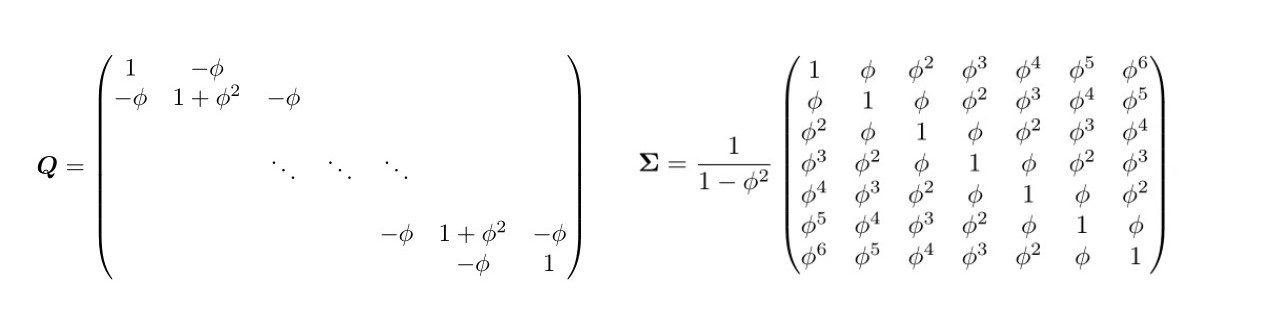
\includegraphics{images/precvscov.jpg}
\caption{\label{fig:precisionmat}Precision Matrix in GMRF vs the Covariance matrix, source \citet{GMRFRue}}
\end{figure}

with zero entries outside the diagonal (right panel fig.~\ref{fig:precisionmat}) and first off-diagonals \citeyearpar{GMRFRue}.
The conditional independence assumption makes the precision matrix tridiagonal since for generals \(\eta_i\) and \(\eta_j\) are conditionally independent for \(|i − j| > 1\), given all the rest. In other words \(\boldsymbol{Q}\) is sparse since given all the latent predictors in \(\boldsymbol\eta\), then \(\eta_t\) depends only on the preceding \(\eta_{t-1}\). For example in \eqref{eq:conditinal}, let assume to have \(\eta_2\) and \(\eta_4\), then:

\begin{equation} 
\begin{split}
  \pi\left(\eta_{2}, \eta_{4} \mid \eta_{1}, \eta_{3}\right) &=\pi\left(\eta_{2} \mid \eta_{1}\right) \pi\left(\eta_{4} \mid \eta_{1}, \eta_{2}, \eta_{3}\right) \\
  & =\pi\left(\eta_{2} \mid \eta_{1}\right) \pi\left(\eta_{4} \mid \eta_{3}\right)
\end{split}
\label{eq:conditinal}
\end{equation}

For which the conditional density of \(\eta_2\) does only depend on its preceding term i.e.~\(\eta_1\). The same inner reasoning can be done for \(\eta_4\), which strictly depends on \(\eta_3\) and vice versa.
Therefore ultimately it is possible to produce a rather formal definition of a GMRF:

\begin{definition}[GMRF]
\protect\hypertarget{def:gmrf}{}{\label{def:gmrf} \iffalse (GMRF) \fi{} }A latent gaussian random field (LGRM) e.g.~\(\boldsymbol\eta = \boldsymbol\theta\) (when \(\mathscr{g}(\cdot)\) is identity) is said a GMRF if it has a multivariate Normal density with additional conditional independence (also called the ``Markov property'') \citep{wang2018bayesian}.
\end{definition}

\[
\pi(\boldsymbol{\theta} \mid \boldsymbol{\psi}_2) = \operatorname{MVN}(0, \boldsymbol{Q(\psi_2}))
\]

\hypertarget{approx}{%
\section{INLA Laplace Approximations}\label{approx}}

The goals of the Bayesian inference are the marginal posterior distributions for each of the elements of the latent field. INLA is not going to try to approximate the whole joint posterior marginal distribution from expression \eqref{eq:finallgm} i.e.~\(\pi(\boldsymbol{\theta} \mid \boldsymbol{\psi}, \boldsymbol{\mathbf{y}})\), in fact if it would (two-dimensional approx) it will cause a high biased approximations since it fail to capture both location and skewness in the marginals. Instead INLA algorithm will try to estimate the posterior marginal distribution for each \(\theta_{i}\) in the latent parameter \(\boldsymbol{\theta}\), for each hyper-parameter prior \(\psi_{k} \in \boldsymbol\psi\) (back to the \(\boldsymbol\theta\) latent field notation).

The mathematical intuition behind \textbf{Laplace Approximation} along with some real life cases are contained in the appendix in sec.~\ref{laplaceapprox}.

Therefore the key focus of INLA is to approximate with Laplace only densities that are near-Gaussian \citeyearpar{wang2018bayesian} or replacing very nested dependencies with their more comfortable conditional distribution which ultimately are ``more Gaussian'' than the their joint distribution.
Into the LGM framework let us assume to observe \(n\) counts, i.e.~\(\mathbf{y} = y_i = 1,2, \ldots, n\) drawn from Poisson distribution whose mean is \(\lambda_i, \forall i \in \mathbf{I}\). Then a the link function \(\mathscr{g}(\cdot)\) is the \(\log()\) and relates \(\lambda_i\) with the linear predictor and so the latent filed \(\theta\), i.e.~\(\log(\lambda_i)=\theta_{i}\). The hyper-parameters are \(\boldsymbol\psi = (\tau, \rho)\) with their covariance matrix structure.
\[
Q_{\psi}=\boldsymbol\tau\begin{bmatrix}
1 & - \rho & - \rho^{2} & - \rho^{3} & \ldots & - \rho^{n} &  \\
- \rho & 1 & - \rho & - \rho^{2} & - \rho^{3} & - \rho^{n-1} & \\
- \rho^{2} & - \rho & 1 & - \rho & - \rho^{2} & - \rho^{n-2} &  \\
- \rho^{3} & - \rho^{2} & - \rho & 1 & - \rho & - \rho^{n-3} &  \\
- \ldots & - \rho^{3} & - \rho^{2} & - \rho & 1 & - \rho &  \\
- \rho^{n} & - \rho^{n-1} & - \rho^{n-2} & - \rho^{n-3} & - \rho & 1 \\
\end{bmatrix}
\]

Let us also to assume once again to model \(\boldsymbol\theta\) with an AR(1).
Then fitting the model into the LGM, at first requires to specify an exponential family distribution function, i.e.~Poisson on the response \(\mathbf{y}\).
then the \emph{higher} level (recall last part sec.~\ref{LGM}) results in:

\[
\pi(\boldsymbol{\mathbf{y}} \mid \boldsymbol{\theta} , \boldsymbol{\psi}) \propto\prod_{i=1}^{\mathbf{I}} \frac{ \exp \left(\theta_{i} y_{i}-e^{\theta_{i}}\right) }{y_{i} !}
\]

Then the \emph{medium} level is for the latent Gaussian Random Field a multivariate gaussian distribution \(\boldsymbol{\psi}_{i} \sim \operatorname{MVN}_{2}(\mathbf{0}, \boldsymbol{Q}_{\boldsymbol{\psi}})\):

\[
\pi(\boldsymbol{\theta} \mid \boldsymbol{\psi}) \propto\left|\boldsymbol{Q}_{\boldsymbol{\psi}}\right|^{1 / 2} \exp \left(-\frac{1}{2} \boldsymbol{\theta}^{\prime} \boldsymbol{Q}_{\boldsymbol{\psi}} \boldsymbol{\theta}\right)
\]
and the \emph{lower}, where it is specified a joint prior distribution for \(\boldsymbol\psi = (\tau, \rho)\), which is \(\pi(\boldsymbol\psi)\). Following eq.\eqref{eq:formallgm} then:

\begin{equation}
\pi(\boldsymbol{\theta}, \boldsymbol{\psi} \mid \mathbf{y})\propto  \underbrace{\pi(\boldsymbol{\psi})}_{\text {priors}} \times \underbrace{\pi(\boldsymbol\theta \mid \boldsymbol\rho)}_{\text {GMRF}} \times \underbrace{\prod_{i=1}^{\mathbf{I}} \pi\left(\mathbf{y} \mid \boldsymbol\theta, \boldsymbol{\tau}\right)}_{\text {likelihood }}
\label{eq:poissonlgm}
\end{equation}

Then recalling the goal for Bayesian Inference, i.e.approximate posterior marginals for \(\pi\left(\theta_{i} \mid \mathbf{y}\right)\) and \(\pi\left(\tau \mid \boldsymbol{\mathbf{y}}\right)\) and \(\pi\left(\rho \mid \boldsymbol{\mathbf{y}}\right)\). First difficulties regard the fact that Laplace approximations on this model implies the product of a Gaussian distribution and a non-gaussian one. As the INLA key point suggest, the algorithm starts by rearranging the problem so that the ``most Gaussian'' are computed at first.
Ideally the method can be generally subdivided into three tasks. At first INLA attempts to approximate \(\tilde{\pi}(\boldsymbol{\psi} \mid \boldsymbol{\mathbf{y}})\) as the joint posterior of \({\pi}(\boldsymbol{\psi} \mid \boldsymbol{\mathbf{y}})\). Then subsequently will try to approximate \(\tilde{\pi}\left(\theta_{i} \mid \boldsymbol\psi, \mathbf{y}\right)\) to their conditional marginal distribution fro \(\theta_i\). In the end explores \(\tilde{\pi}(\boldsymbol{\psi} \mid \boldsymbol{\mathbf{y}})\) with numerical methods for integration.
The corresponding integrals to be approximated are:

\begin{itemize}
\tightlist
\item
  for task 1: \(\pi\left(\psi_{k} \mid \boldsymbol{\mathbf{y}}\right)=\int \pi(\boldsymbol{\psi} \mid \boldsymbol{\mathbf{y}}) \mathrm{d} \boldsymbol{\psi}_{-k}\)
\item
  for task 2: \(\pi\left(\theta_{i} \mid \boldsymbol{\mathbf{y}}\right)=\int \pi\left(\theta_{i}, \boldsymbol{\psi} \mid \boldsymbol{\mathbf{y}}\right) \mathrm{d} \boldsymbol{\psi}=\int \pi\left(\theta_{i} \mid \boldsymbol{\psi}, \boldsymbol{\mathbf{y}}\right) \pi(\boldsymbol{\psi} \mid \boldsymbol{\mathbf{y}}) \mathrm{d} \boldsymbol{\psi}\)
\end{itemize}

As a result the approximations for the marginal posteriors are at first:

\begin{equation}
\tilde{\pi}\left(\theta_{j} \mid \boldsymbol{\mathbf{y}}\right)=\int \tilde{\pi}(\boldsymbol{\theta} \mid \boldsymbol{\mathbf{y}}) d \boldsymbol{\theta}_{-j}
\label{eq:postapproxprior}
\end{equation}

and then,

\begin{equation}
\tilde{\pi}\left(\theta_{i} \mid \boldsymbol{\mathbf{y}}\right) \approx \sum_{j} \tilde{\pi}\left(\theta_{i} \mid \boldsymbol{\psi}^{(j)}, \boldsymbol{\mathbf{y}}\right) \tilde{\pi}\left(\boldsymbol{\psi}^{(j)} \mid \boldsymbol{\mathbf{y}}\right) \Delta_{j}
\label{eq:postapproxlatent}
\end{equation}

Where in the integral in \eqref{eq:postapproxlatent} \(\{\boldsymbol{\psi}^{(j)}\}\) are some relevant integration points and \(\{\Delta_j\}\) are weights associated to the set of hyper-parameters ina grid. \citep{Blangiardo-Cameletti}.
In other words the bigger the \(\Delta_{j}\) weight the more relevant are the integration points. Details on how INLA finds those points is beyond the scope, an indeep resource if offered by \citet{wang2018bayesian} in sec.~2.3.

\hypertarget{rinla}{%
\section{R-INLA package}\label{rinla}}

INLA library and algorithm is developed by the R-INLA project whose package is available on their website at their \href{https://www.r-inla.org/download-install}{source repository}. Users can also enjoy on INLA website (recently restyled) a dedicated forum where discussion groups are opened and an active community is keen to answer. Moreover It also contains a number of reference books, among which some of them are fully open sourced. INLA is available for any operating system and it is built on top of other libraries still not on CRAN.
The core function of the package is \passthrough{\lstinline!inla()!}and it works as many other regression functions like \passthrough{\lstinline!glm()!}, \passthrough{\lstinline!lm()!} or \passthrough{\lstinline!gam()!}. Inla function takes as argument the \emph{model formula} i.e.~the linear predictor for which it can be specified a number of linear and non-linear effects on covariates as seen in eq. \eqref{eq:linearpredictor}, the whole set of available effects are obtained with the command \passthrough{\lstinline!names(inla.models()$latent)!}. Furthermore it requires to specify the dataset and its respective likelihood family, equivalently \passthrough{\lstinline!names(inla.models()$likelihood)!}.
Many other methods in the function can be added through lists, such as \passthrough{\lstinline!control.family!} and \passthrough{\lstinline!control.fixed!} which let the analyst specifying parameter and hyper-paramenters priors family distributions and control hyper parameters. They come in the of nested lists when parameters and hyper paramenters are more than 2, when nothing is specified the default option is non-informativeness.
Inla output objects are inla.dataframe summary-lists-type containing the results from model fitting for which a table is given in figure \ref{fig:summartable}.

\begin{figure}
\centering
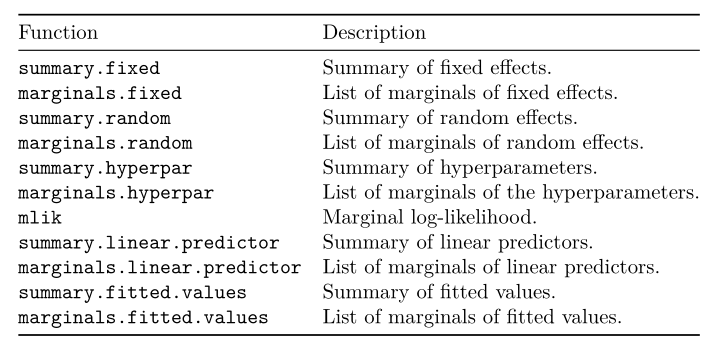
\includegraphics{images/summarytable.PNG}
\caption{\label{fig:summartable}outputs for a \passthrough{\lstinline!inla()!} call, source: \citet{Krainski-Rubio}}
\end{figure}

SPDEtoy dataset \(\mathbf{y}\) are two random variables that simulates points location in two coordinates \(s_1\) and \(s_2\).

\begin{figure}

{\centering 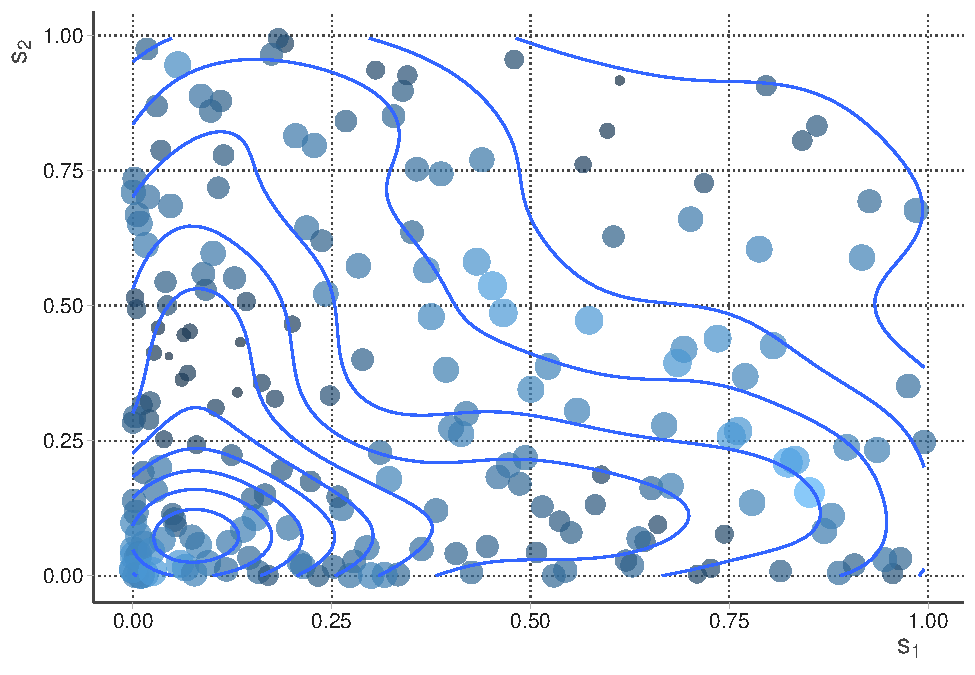
\includegraphics{04-inla_files/figure-latex/spatplot-1} 

}

\caption{SPDEtoy bubble plot, author's source}\label{fig:spatplot}
\end{figure}

Imposing an LGM model requires at first to select as a \emph{higher} hierarchy level a likelihood model for \(\mathbf{y}\) i.e.~Gaussian (by default), and a model formula (eq. \eqref{eq:linearpredictor}), i.e.~\(\eta_{i}=\beta_{0}+\beta_{1} s_{1 i}+\beta_{2} s_{2 i}\), which link function \(\mathbf{g}\) is identity. There are not Non-linear effects effect on covariates in \$\eta \$ nevertheless they can be easily added with \passthrough{\lstinline!f()!} function. Note that this will allow to integrate random effects i.e.~spatial effects inside the model. Secondly in the \emph{medium} step a LGRF on the latent parameters \(\boldsymbol\theta\). In the \emph{lower} end some priors distributions \(\boldsymbol\psi\) which are Uniform for the intercept indeed Gaussian vagues (default) priors i.e.~centered in 0 with very low standard deviation. Furthermore the precision hyper parameter \(\tau\) which accounts for the variance of the latent GRF, is set as Gamma distributed with parameters \(\alpha = 1\) and \(\beta = 0.00005\) (default). Note that models are sensitive to prior choices (sec.~\ref{priorsspec}), as a consequence if necessary later are revised.
A summary of the model specifications are set below:

\begin{equation} 
\begin{split}
y_{i} & \sim N\left(\mu_{i}, \tau^{-1}\right), i=1, \ldots, 200 \\
\mu_{i} &=\beta_{0}+\beta_{1} s_{1 i}+\beta_{2} s_{2 i} \\
\beta_{0} & \sim \text { Uniform } \\
\beta_{j} & \sim N\left(0,0.001^{-1}\right), j=1,2 \\
\tau & \sim G a(1,0.00005)
\end{split}
\end{equation}

Then the model is fitted within \passthrough{\lstinline!inla()!} call, specifying the formula, data and the exponential family distribution.

\begin{lstlisting}[language=R]
formula = y ~ s1 + s2
m0 = inla(formula, data = SPDEtoy, family = "gaussian")
\end{lstlisting}

Table \ref{tab:tableINLA} offers summary of the posterior marginal values for intercept and covariates' coefficients, as well as precision. Marginals distributions both for parameters and hyper-parameters can be conveniently plotted as in figure \ref{fig:postplot}. From the table it can also be seen that the mean for \(s_2\) is negative, so the Norther the y-coordinate, the less is response. That is factual looking at the SPDEtoy contour plot in figure \ref{fig:spatplot} where bigger bubbles are concentrated around the origin.

\begin{table}

\caption{\label{tab:tableINLA}Summary Posterior quantiles for coefficients}
\centering
\begin{tabular}[t]{lrr}
\toprule
coefficients & mean & sd\\
\midrule
(Intercept) & 10.1321487 & 0.2422118\\
s1 & 0.7624296 & 0.4293757\\
s2 & -1.5836768 & 0.4293757\\
\bottomrule
\end{tabular}
\end{table}

\begin{figure}

{\centering 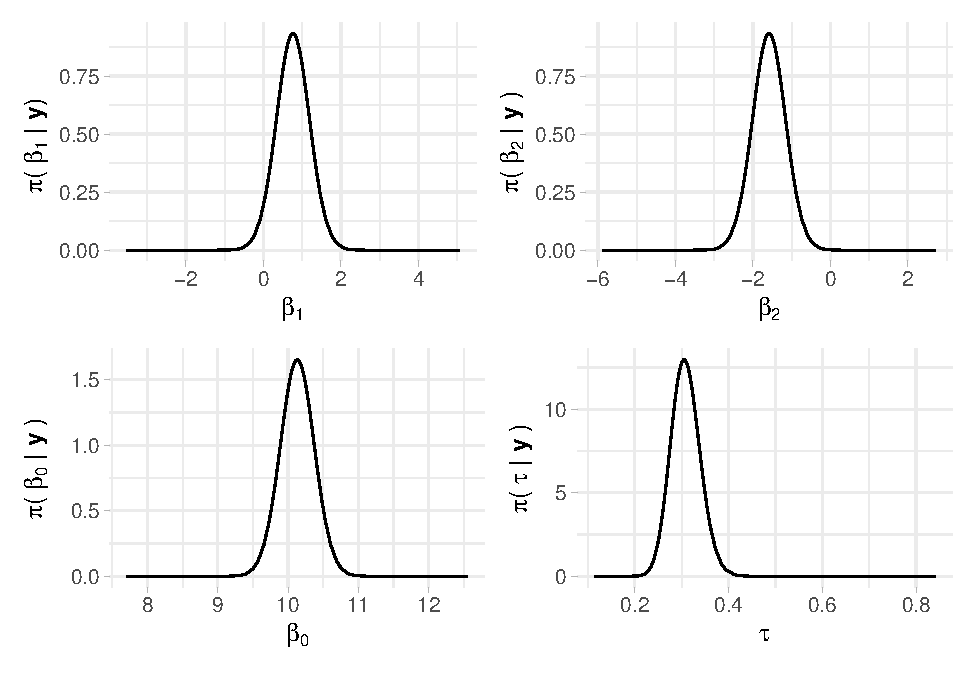
\includegraphics{04-inla_files/figure-latex/postplot-1} 

}

\caption{Linear predictor marginals, plot recoded in `ggplot2`, author's source}\label{fig:postplot}
\end{figure}

In the end R-INLA enables also r-base fashion function to compute statistics on marginal posterior distributions for the density, distribution as well as the quantile function respectively with \passthrough{\lstinline!inla.dmarginal!}, \passthrough{\lstinline!inla.pmarginal!} and \passthrough{\lstinline!inla.qmarginal!}. One option which allows to compute the higher posterior density credibility interval \passthrough{\lstinline!inla.hpdmarginal!} for a given covariate's coefficient i.e, \(\beta_2\), such that \(\int_{q_{1}}^{q_{2}} \tilde{\pi}\left(\beta_{2} \mid \boldsymbol{y}\right) \mathrm{d} \beta_{2}=0.90\) (90\% credibility), whose result is in table below.

\begin{table}

\caption{\label{tab:higerPosteriorDensityInterval}Higer Posterior Density Interval for s2 coefficient}
\centering
\begin{tabular}[t]{lrr}
\toprule
  & low & high\\
\midrule
level:0.9 & -2.291268 & -0.879445\\
\bottomrule
\end{tabular}
\end{table}

Note that the interpretation is more convoluted \citeyearpar{wang2018bayesian} than the traditional frequentist approach: in Bayesian statistics \(\beta_{j}\) comes from probability distribution, while frequenstists considers \(\beta_{j}\) as fixed unknown quantity whose estimator (random variable conditioned to data) is used to infer the value \citeyearpar{Blangiardo-Cameletti}.

\hypertarget{prdm}{%
\chapter{Geostatistical Data Analysis}\label{prdm}}

Geostatistical or equivalently point reference data are a collection of samples indexed by coordinates pertaining to a spatially continuous surface \citep{Moraga2019}. Coordinates might be in the form of Latitude and Longitude or Eastings and Northings, moreover they can be also unprojected with respect to a Coordinate Reference Systems (CRS e.g.~lat and log), or projected (e.g.~East. and North.). Data as such can monitor a vast range of phenomena, e.g.~accidental fisheries bycatch for endangered species \citep{CosandeyGodin2015}, COVID19 severity and case fatality rates in Spain \citep{Moragacovid2020}, PM10 pollution concentration in a North-Italian region Piemonte \citep{Cameletti2012}. Moreover a large geostatistical application takes place on Real Estate e.g.~Boston house prices lattice data \citep{mass} are ingested by several spatial models \citep{rubiorealestate}, or spatio-temporal modeling for apartment transaction prices in Corsica (FR) \citep{Ling}. All the examples taken before have implied inla and might have documented a spatial nature of data according to which closer observations were displaying similar values. This phenomenon is named spatial autocorrelation. Spatial autocorrelation conceptually stems from geographer Waldo Tobler whose famous quote, known as first law of geography, inspires geostatisticians:

\begin{quote}
``Everything is related to everything else,
but near things are more related than distant things''

\hfill --- Waldo R. Tobler
\end{quote}

Spatial data can be partitioned into three main types, even tough they all fall under the umbrella of inla algorithm, indeed each employs context specific tools.

\begin{itemize}
\tightlist
\item
  Areal Data
\item
  \textbf{Point Referenced Data}
\item
  Point Pattern Data
\end{itemize}

\begin{figure}
\centering
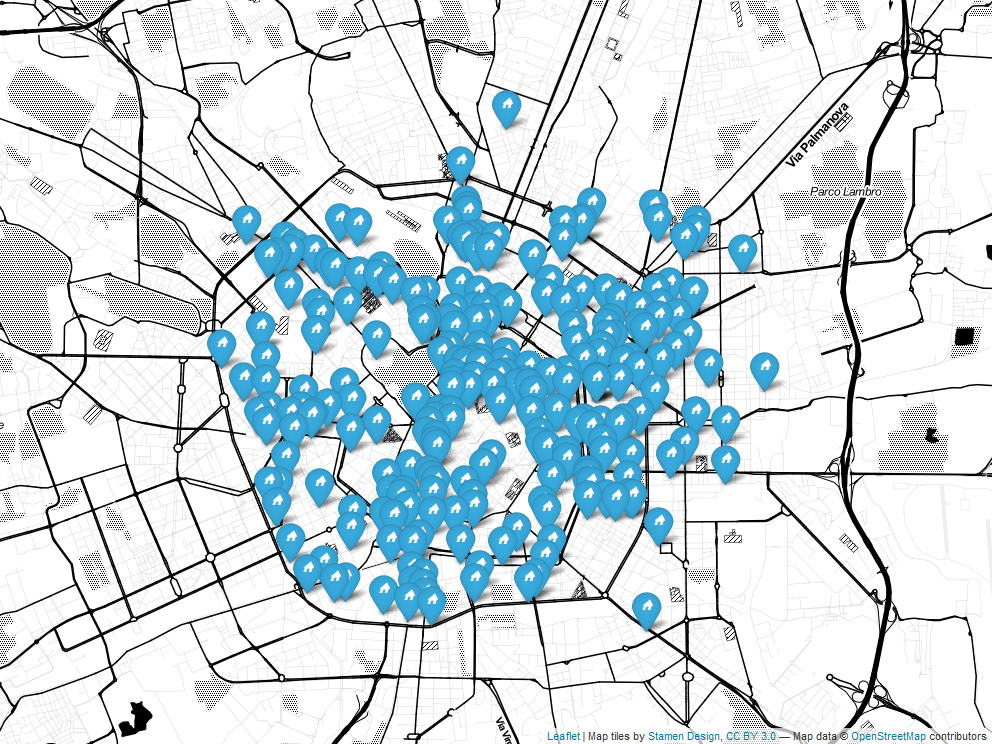
\includegraphics{images/map.png}
\caption{\label{fig:prdmap}Point Referenced Data map plot (\passthrough{\lstinline!Leaflet!} \citet{leaflet}) of a RESTful API call on Milan Rental Real Estate 20-11-2019, Author's Source}
\end{figure}

In this chapter Gaussian Processes are seen as the continuous surface from which point referenced data are the partial realization. At first they are defined, then aer constrained to the properties of Stationarity and Isotropy. Furthermore they are considered with a suitable covariance function, i.e.~Matèrn that uncovers convenient properties. These properties and the reason why Matérn is selected as candidate relies, besides its inner flexibility, on the fact that GP whose covariance function is Matérn are able to determine a GMRF \ref{gmrf} representation of the process through the Stochastic Partial Differential Equations (SPDE) approach \citep{Lindgren2011}. The main benefit proceeding from a GP to a GMRF arises from the good computational properties that the latter appreciate enabling to wrap up modeling around INLA and consequently benefiting from its speed. Hedonic Price Models brings to the present analysis the theoretical foundation according to which covariates are added to the model. Then model criticism in the context of INLA is reviewed introducing two methodologies to assess model suitability based on predictive posterior distribution and deviance. In the end the prior choice falls on penalized complexity priors \citep{simpson2017} which constitutes a set of effective guidelines to choose priors that are compatible and natively implemented in INLA.

\hypertarget{GP}{%
\section{Gaussian Process (GP)}\label{GP}}

Geostatistical data are defined as realizations of a stochastic process indexed by space.

\[
Y(s) \equiv\{y(s), s \in \mathscr{D}\}
\]
where \(\mathscr{D}\) is a (fixed) subset of \(\mathbb{R}^{d}\) (in the present work \emph{Latitude} and \emph{Longitude}, i.e.~\(d=2\)). The actual data can be then represented by a collection of observations \(\boldsymbol{\mathbf{y}}=\left\{y\left(s_{1}\right), \ldots, y\left(s_{n}\right)\right\}\) (recall notation from previous chapter \ref{LGM}) where the set \(\left(s_{1}, \ldots, s_{n}\right)\) points to the spatial location where data has been observed. For example, following \citet{Cameletti2012}, let us assume to have collection of samples from air pollutant measurements obtained by observing a set of monitoring stations. Then The stochastic process \(Y(s)\) is monitored in a fixed set of spatial indexes corresponding to the station locations (upword arrows left in figure \ref{fig:prdproc}). This information is essential to interpolate points and build a spatially continuous surface (right panel in figure \ref{fig:prdproc}) over the y-studied variable domain in order to predict the phenomenon at locations not yet observed \citep{LecturePaci}. Note that notation such as \(Y(s_i)\) from now on will be discarded in favor of the subscript for the correspondent observation indexes i.e.~\(Y_i\).

\begin{figure}
\centering
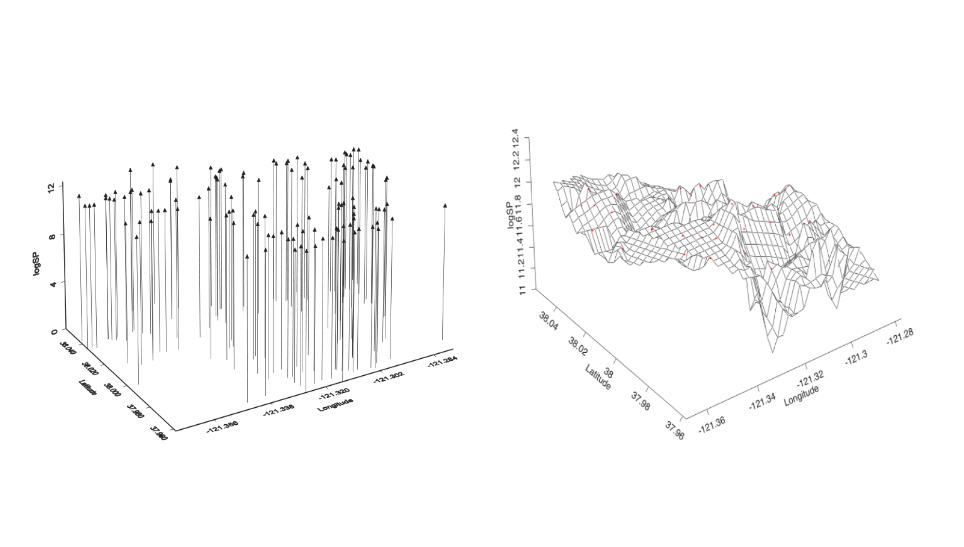
\includegraphics{images/prdprocess.png}
\caption{\label{fig:prdproc}Stockton data, Left: Spatial drop line scatterplot projected into the \(3^{rd}\) dim \(\log(Price)\), Right: its three-dimensional surface , source \citet{Blangiardo-Cameletti}}
\end{figure}

The first step in defining a spatial model within INLA is to impose a LGM hierarchical structure which requires at first to identify a probability distribution function for the observed data \(\boldsymbol{\mathbf{y}}\), i.e.~higher level. The most common choice is to draw distributions from the \emph{Exponential family}, indexed by a set of parameters \(\boldsymbol\theta\) as in \ref{LGM}, accounting for the spatial correlation.
In the case of geostatistical data, the model parameters \(\boldsymbol\theta\), following notation imposed in chapter \ref{inla} are defined as a latent Gaussian Process (GP). Then a formal definition of GP is given,

\begin{definition}[GP definition]
\protect\hypertarget{def:GP}{}{\label{def:GP} \iffalse (GP definition) \fi{} }A collection of \(n\) random variables, such as \(Y(s_{1}), Y(s_{2}) , \ldots, Y(s_{n})\) that are \emph{valid} and \emph{finite} stochastic processes are said to be a \textbf{GP} if for any set of spatial index \(n\) and for each set of corresponding locations \(\left\{y\left(s_{1}\right), \ldots, y\left(s_{n}\right)\right\}\) follows a \emph{Multivariate Gaussian} distribution with mean \(\boldsymbol{\mu}=\left\{\mu\left(s_{1}\right), \ldots, \mu\left(s_{n}\right)\right\}\) and covariance matrix \(\mathbf{Q}^{-1}_{i,j}, \forall i \neq j\) defined then by a covariance function \(\mathscr{\cdot, \cdot}\) i.e.~
\end{definition}

The latent GP are in function of some hyper-parameters \(\boldsymbol\psi\) and their respective prior \(\pi(\boldsymbol\psi)\). Moreover a GP is completely characterized by a mean \(\boldsymbol{\mu}=\left(\mu_{1}, \ldots, \mu_{n}\right)^{\prime}\) and a spatially structured covariance matrix \(\boldsymbol{Q^{-1}}\), whose generic element is \(\boldsymbol{Q^{-1}}_{i j}=\operatorname{Cov}(\theta_{i}, \theta_{j})=\sigma^2_{\mathscr{\boldsymbol{\mathbf{y}}}} \mathscr{C}(\Delta_{i j})\), where \(\sigma_{\mathscr{\boldsymbol{\mathbf{\xi}}}}^{2}\) is the variance component of the process and for \(i, j = 1, \ldots, n\). \(\mathscr{C}\left( \cdot, \cdot \right)\) function generally ensures that all the values that are close together in input space will produce output values that are close together, by inheriting the \emph{validity} and \emph{positive definitness} characteristics from the GP. The spatial stochastic process commonly is assumed to fulfill two important properties: \textbf{stationary}, \textbf{Isotropy} (even tough both of the two can be relaxed).
A process is said \textbf{stationary} i.e.~weak stationary, if process values at any two locations can be summarized by a covariance function \(\mathscr{C(\Delta_{i j})}\) depending solely on the distance. In other words it is invariant under \emph{translation} \citep{Krainski-Rubio}.
A process is said \textbf{Isotropical} if the covariance function depends only on the between-points distance \(\Delta_{i j}=\left\|s_{i}-s_{j}\right\|\) (in this context \emph{Euclidean}), so it is invariant under \emph{rotation} \citeyearpar{Krainski-Rubio}. A further way of seeing this property is that Isotropy causes to stochastic processes concentric decaying contours \citep{LecturePaci}, green in fig.~\ref{fig:isoovsanis}, meaning the vanishing of spatial dependence \citep{Blangiardo-Cameletti}, and so for covariance values.

\begin{figure}
\centering
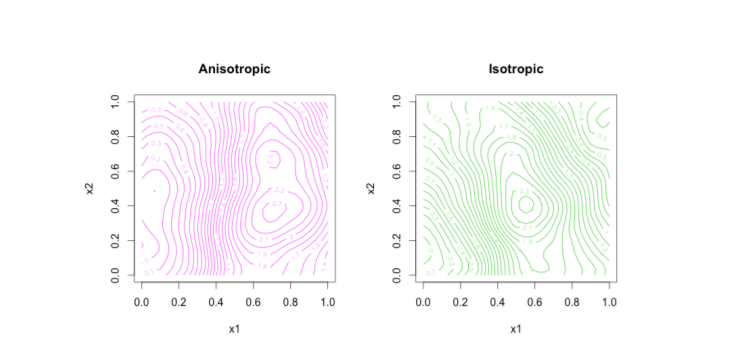
\includegraphics{images/isotropyVSanisotropy.png}
\caption{\label{fig:isoovsanis}Left: anisotropical concentric decaying contours, Right: isotropical concentric decaying contours , source \citet{blanchetscalliet}}
\end{figure}

In spatial statistics the isotropical assumption is very frequent despite being restrictive for describing the rich variety of interactions that can characterize spatial processes. Anyway assuming the property it offers a wide range of underlying functions that can model spatial dependence for which three are the most common ones \citep{Krainski2018}

\[
\begin{aligned}
&\text { Exponential } \quad \mathscr{C}(\Delta_{i j})=\left\{\begin{array}{cl}
\tau^{2}_{\mathscr{C}}+\sigma^{2}_{\mathscr{C}} & \text { if }  \Delta_{i j}=0 \\
\sigma^{2}_{\mathscr{C}} \exp (-\phi_{\mathscr{C}} \Delta_{i j}) & \text { if } \Delta_{i j}>0 
\end{array}\right.\\
&\text { Gaussian } \quad \mathscr{C}(\Delta_{i j})=\left\{\begin{array}{cl}
\tau^{2}_{\mathscr{C}}+\sigma^{2}_{\mathscr{C}} & \text { if } \Delta_{i j}=0 \\
\sigma^{2}_{\mathscr{C}} \exp \left(-\phi^{2}_{\mathscr{C}}  \Delta_{i j}^{2}\right) & \text { if } \Delta_{i j}>0 
\end{array}\right. \\
&\text { Matérn } \quad \mathscr{C}(\Delta_{i j})=\left\{\begin{array}{cl}
\tau^{2}_{\mathscr{C}}+\sigma^{2}_{\mathscr{C}} & \text { if } \Delta_{i j}=0 \\
\frac{\sigma^{2}_{\mathscr{C}}}{\Gamma(\nu) 2^{\nu-1}}(\phi_{\mathscr{C}}  \Delta_{i j})^{\nu} K_{\nu}(\phi_{\mathscr{C}}  \Delta_{i j}) & \text { if } \Delta_{i j}>0
\end{array}\right.
\end{aligned}
\]

where all the parameters above are special quantities derived from the emphirical variogram. \(\sigma^2\), \(\tau^2\), \(\phi^2\), and are respectively the \emph{range}, the distance at which correlation vanishes, the \emph{nugget}, i.e.~the non spatial variance and the \emph{partial sill}, i.e.~the spatial effect variance \citep{LecturePaci}.
In particular the focus is on the \emph{Matérn} -- as it is required by the SPDE approach in section \ref{spdeapproach} -- and this should not be intended as a restriction. In fact, as long described in \citet{gneiting2006geostatistical}, the Matèrn family is a very flexible class. Matérn is tuned mainly by two hyper-parameters, a scaling one \(\phi>0\), usually set equal to the range of the spatial process \(\sigma^{2}_{var}\) i.e.~the distance at which the spatial dependence becomes negligible, by the empirically derived relation \(r =\frac{\sqrt{8 \lambda}}{\kappa}\)), and a smoothing one \(\nu>0\) usually kept fixed. An \emph{isotropical} and \emph{stationary} Matérn covariance expression by isolating the variance of the spatial process \(\sigma_{\mathscr{\boldsymbol{\mathbf{\xi}}}}^{2}\) is:

\[
\begin{aligned}
\text { Matérn } \quad \mathscr{C}( \Delta_{i j})= \sigma_{\mathscr{\boldsymbol{\mathbf{\xi}}}}^{2} \left\{\begin{array}{cl}
\tau^{2}_{\mathscr{C}} & \text { if } \Delta_{i j}=0 \\
\frac{1}{\Gamma(\nu) 2^{\nu-1}}\left(\phi \Delta_{i j}\right)^{\nu} K_{\nu}\left(\phi \Delta_{i j}\right)& \text { if } \Delta_{i j}>0
\end{array}\right.
\end{aligned}
\]

\(\Gamma(\nu)\) is a Gamma function depending on \(\nu\) values and \(K_{\nu}(\cdot)\) is a modified Bessel function of second kind \citep{yaşar2016unified}. The scaling parameter \(\phi\) in figure \ref{fig:matern} takes 4 different values showing the flexibility of Matérn to relate different distances according to varying parameters, while \(\nu\) is kept to the value of \(.5\) and addresses the GP degree of smoothness.
Looking at the functions in figure \ref{fig:matern} and their interception with horizontal red line, when \(\phi = 1\), it smoothly falls towards 0 covariance and spatial dependece decays at \(\approx 2.3\). When \(\phi = 1/2\) it becomes the exponential covariance function and rapidly pushes covariance to 0, When \(\phi = 3/2\) it uncovers a convenient closed form \citep{LecturePaci} for which spatial dependence vanishes at \(\approx 3.8\). When \(\phi \approx \infty\), (here \(\phi = 80\) for graphics reasons), it becomes Gaussian covariance function. In the the case shown in section \ref{spdeapproach} \(\sigma_{\mathscr{C}}^{2}\) the range, for any \(\phi\), is set equal to the distance at which dependence vanishes below .1, which is actually what the red line points out.

\begin{figure}

{\centering 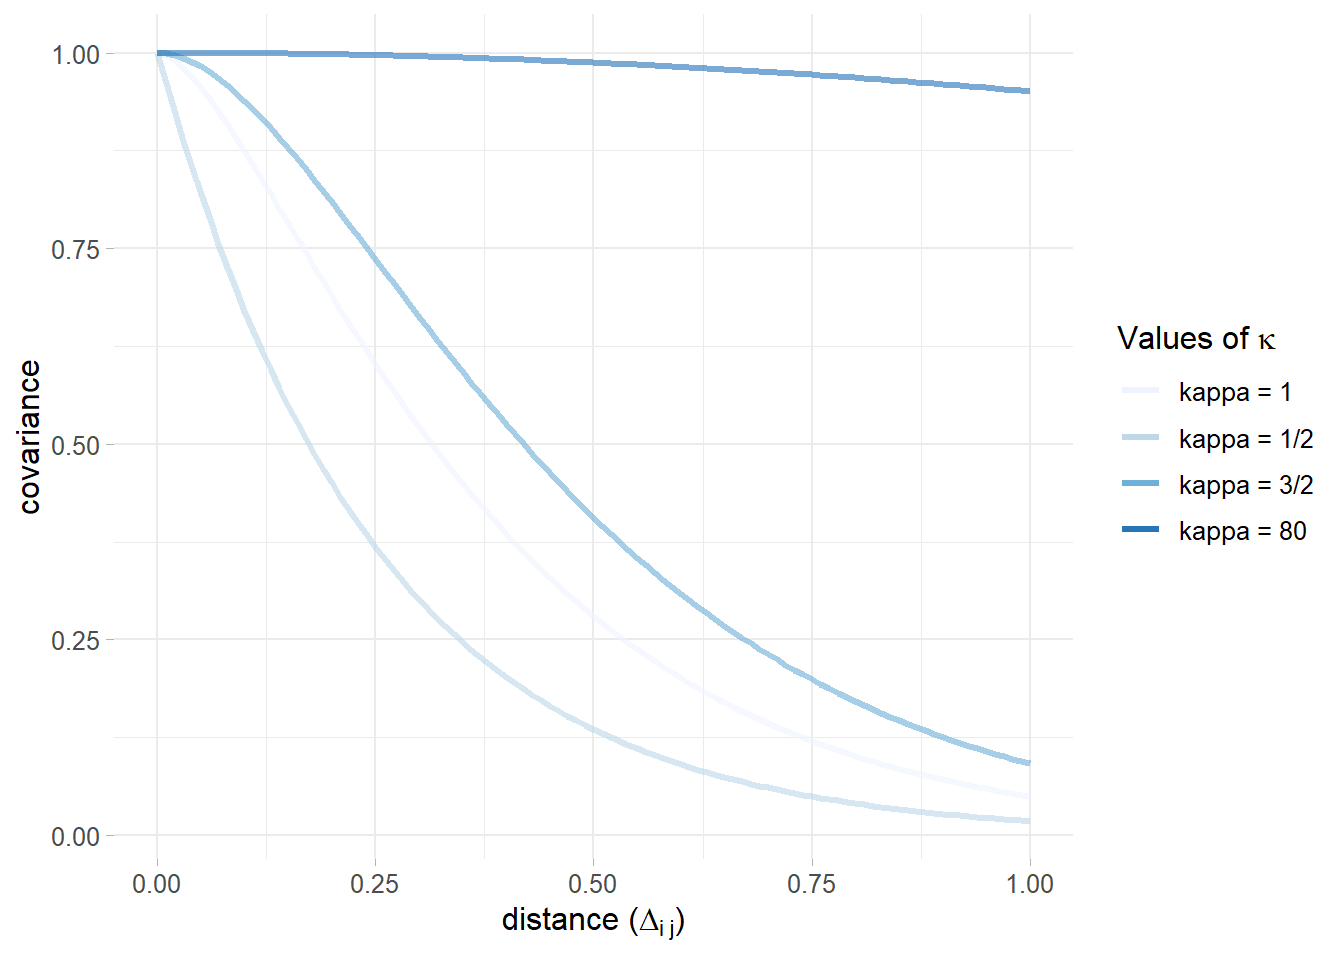
\includegraphics{05-prd_modelling_files/figure-latex/matern-1} 

}

\caption{Matérn covariance function for 4 different phi values and fixed nu = .5, dashed red horizontal line when covariance is .1}\label{fig:matern}
\end{figure}

In the end summarizing the result obtained (abuse of notation with \((s)\) to make it clear that is a spatial process) in chapter \ref{inla} with what it has been seen so far, the Gaussian process \(y(s)\) assumes the following measurement equation, where \(\xi_{i}\) is the latent field, \(\varepsilon_{t} \sim N\left(\mathbf{0}, \sigma_{\varepsilon}^{2} I_{d}\right)\) is the white noise error and \(I_{d}\) is an identity matrix and \(\xi(\boldsymbol{s})\sim N\left(\mathbf{0}, \boldsymbol{Q^{-1}}=\sigma_{\xi}^{2} \mathscr{C}( \Delta_{i j})\right)\).

\[
y(s)=\boldsymbol{z}(\boldsymbol{s}) \boldsymbol{\beta}+\xi(\boldsymbol{s})+\varepsilon(\boldsymbol{s})
\]

\hypertarget{spdeapproach}{%
\section{The Stochastic Partial Differential Equation (SPDE) approach}\label{spdeapproach}}

Locations in the spatial setting are considered as realizations of a stationary, isotropical unobserved GP to be estimated (\ref{GP}). Before approaching the problem with SPDE, GPs were treated as multivariate Gaussian densities and Cholesky factorizations were applied on the covariance matrices and then fitted with likelihood \citep{LecturePaci}. Covariance matrices in the context of spatial and spatio-temporal models \citep{PACI2017149, Cameletti2012} are \(n \times n\) dimension matrices defined by the number of observations at each single point location (at each time stamp in spatio-temporal) \citep{BLANGIARDO201339}. Covariance matrix as such are very dense and they were scaling with the order of \(\mathcal{O}\left(n^{3}\right)\) \citep{Banerjee-Gelfand}. Problem were linked to the computational costs needed for linear algebra operations for model fitting and spatial interpolation as well as prediction \citep{Cameletti2012}, having led to obvious \emph{big-n} problem.
The breakthrough came with \citet{Lindgren2011} that proves that a stationary, isotropical (can be both relaxed at the cost of different settings) GP with Matérn covariance can be represented as a GMRF using SPDE solutions by Finite Element Method \citep{Krainski-Rubio}. In other words given a GP whose covariance matrix is \(\boldsymbol{Q^{-1}}\), SPDE can provide a method to approximate \(\boldsymbol{Q^{-1}}\) without the previous computational constraints. As a matter of fact SPDE are equations whose solutions are GPs with a chosen covariance function focused on satisfying the relationship SPDE specifies \citeyearpar{Krainski-Rubio}.
Benefits are many but the most important is that the representation of the GP through a GMRF provides a sparse representation of the spatial effect through a sparse precision matrix \(\boldsymbol{Q}\) . Sparse matrices enable convenient inner computation properties of GMRF \ref{approx} which are exploited by INLA algorithm \ref{inla} leading to a more feasible big-O \(\mathcal{O}\left(n^{3 / 2}\right)\). Mathematical details and deep understanding of the equations in SPDE are beyond the scope of the analysis. Luckily enough R-INLA has a set of functions that makes clear to the practitioner the minimal requirements to pass from discrete locations to their continuously indexed surface alter-ego.
As a result of SPDE the spatial Matérn field i.e.~the spatial process \(\xi(\boldsymbol{s})\) becomes \(\tilde\xi(\boldsymbol{s})\), where the precision matrix \(Q\) comes from the SPDE representation \citeyearpar{Cameletti2012}.

In few words SPDE approach uses a finite element (FEM method) representation to shape the Matérn field as a linear combination of basis functions defined on a triangulation (Delaunay) of the domain \(\mathcal{D}\) \citeyearpar{Cameletti2012}, also named \emph{mesh}. What it internally does is splitting the domain \(\mathcal{D}\) into a number of non-intersecting triangles which converge in a common edge or corner. Then the initial vertices of the triangles are set at \(s_1 \ldots s_d\). In order to get a proper triangulation, useful for spatial prediction, additional vertices are then added. The more vertices are added the more the triangulation is accurate since many more triangles can better interpolate the surface reaching more complex shapes. On the other side the more are the triangle the more it will take to compute the mesh and INLA performances can be damaged.

Secondly SPDE maps with a Projection matrix the values of the triangulation to the discretized spatial surface with weighted sum of areas of the underlying triangles.

A less superficial intuition on how SPDE computes triangularizes values and how it uses the projection matrix based on a weighted sum of basis functions to inject the triangulation into the GRMF is offered in the appendix in section \ref{triangular}.

To illustrate the concept of triangulation \citet{Cameletti2012} provide a scatterplot for Piemonte PM10 concentration observed at 24 monitoring stations left in figure \ref{fig:piepm10}. Its respective mesh using 123 vertices and Piemonte borders is in right figure \ref{fig:piepm10}.

\begin{figure}
\centering
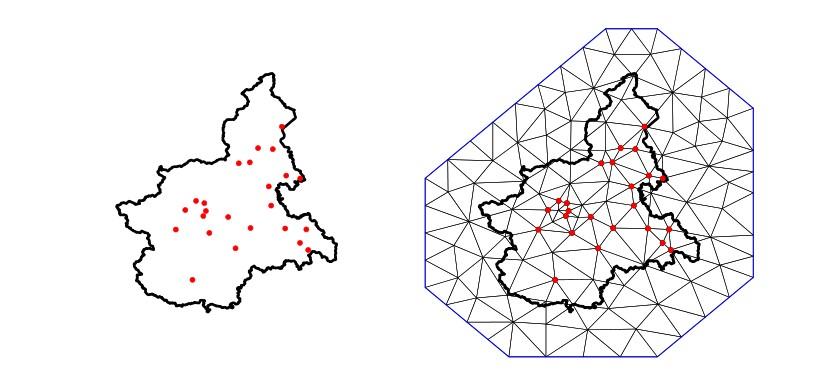
\includegraphics{images/piemonte_pm10.jpg}
\caption{\label{fig:piepm10}Left: monitoring stations in Piemonte region for PM10 pollution levels. Right: its triangulation using 123 vertices. \citet{Cameletti2012} source}
\end{figure}

Any triangle height (the size of the spatial field at each vertex triangle) is calculated by weighted sum, with linear interpolation deciding the values within the triangle. Figure \ref{fig:spdesurf} shows a continously indexed random spatial field (left side of figure \ref{fig:spdesurf}) with the corresponding SPDE on the basis of a triangulation (right panel \ref{fig:spdesurf}).

\begin{figure}
\centering
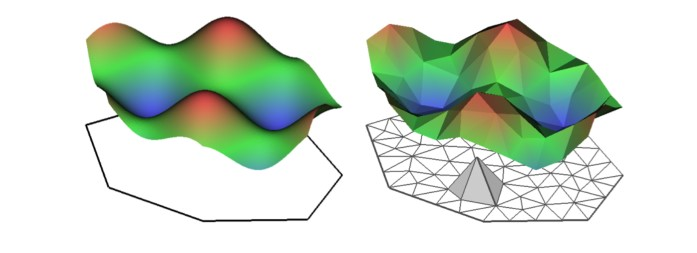
\includegraphics{images/spde_indexedsurface.jpg}
\caption{\label{fig:spdesurf}Left: example of a spatial random field where \(X(s)= \cos(s_1)+\sin(s_2)\), Right: \(X(s)\) SPDE representation given a triangulation, \citet{Cameletti2012} source}
\end{figure}

In INLA mesh triangularization of the region of the study is performed within the function \passthrough{\lstinline!inla.mesh.2d()!}. Main arguments are:

\begin{itemize}
\tightlist
\item
  \passthrough{\lstinline!loc!}: the coordinates used as initial vertices of mesh,
\item
  \passthrough{\lstinline!boundary!}: the borders of the region of the study \(\mathscr{D}\)
\item
  \passthrough{\lstinline!offset!}: the distance between data positions, which determines the inner and outer extension size,
\item
  \passthrough{\lstinline!cutoff!}: minimum distance between points approved.
\item
  \passthrough{\lstinline!max.edge!}: value that suggest the current maximum triangle edge lengths in the area and extension. This argument is on the same scale unit as coordinates.
\item
  \passthrough{\lstinline!min.angle!} the opposite of max.edge
\end{itemize}

Moreover the mesh can also be built on non convex study area by prior passing coordinates on \passthrough{\lstinline!inla.nonconvex.hull()!} which are then sent back to the \passthrough{\lstinline!inla.mesh.2d()!}. A convex hull is a polygon of triangles out of the domain area, in other words the extension made to avoid the boundary effect. If borders are available (and they are) are generally preferred over non convex hull meshes. A decent mesh must have triangles of size and shape as regularly as possible \citep{Krainski-Rubio}.

\hypertarget{hedonic-rental-price-models}{%
\section{Hedonic (rental) Price Models}\label{hedonic-rental-price-models}}

The theoretical foundation of the Hedonic Price Models (from now on HPM) resides in the consumer utility theory of \citet{Lancaster} together with \citet{Rosen} market equilibrium. According to Lancaster the utility of a commodity does not exist by itself, instead it exists as the sum of the utilities associated to its separable characteristics. Integrating Lancater, Rosen introduces HPM and suggests that each separate commodity characteristics are priced by the markets on the basis of supply and demand equilibra. Applying HPM to Real Estate in a market context, from the buy side house prices (indeed also rents) are set as the unit cost of each household attributes, conversely from the selling side the expenditures associated to build of each them.
Formalizing the results, Hedonic Price \(P\) in Real Estate is expressed as a general \(f\) functional form that takes as input the house characteristics vector \(\mathbf{C} = \{c_1,c_2, c_3, \ldots c_n\}\).

\[P=f\left(c_{1}, c_{2}, c_{3}, \ldots, c_{n}\right)\]

Vector \(\mathbf{C}\) since now might contain a unidentified and presumably vast number of ungrouped characteristics. In this setting \citet{Malpezzi} tried to organize house features by decomposing \(\mathbf{C}\) into mutually exclusive and exhaustive subgroups. The vector components involves the house price \(P\), which is in a \(f\) relation with: \(S\), the structural characteristics of the house, \(N\), the neighborhood characteristics, \(L\), the locational characteristics, \(C\), the contract conditions and \(T\) time dimension (not included in the model). \(\beta\) is the vector of the parameters to be estimated. Therefore:

\[P=f\left(S, N, L, C, T, \beta\right)\]
However the critical part of studying house characteristics in geostatistics is the \emph{estimation} and a recent (and not recent) number of emerging trends are observed \citep{SHEPPARD19991595}. Trends, other than the methods presented in this analysis suggests semi-parametric or non-parametric methods and applications of spatial econometrics \citet{Ling}. Researchers would also contend with problems ranging from variable selection to model specification \citeyearpar{Ling}.
For semi-paramametric models a local polynomial regression is developed by \citet{clapp}. The model provides a nonlinear term for the measurement of housing position values dependent on latitudes and longitudes.
Proper geoadditive models family was originally proposed by Kammann and Wand \citeyearpar{kammanwand}, which offers a combination of additive modeling \citep{buja1989} and a geostatistical component. As Ling \citeyearpar{Ling} points out the candidates for the spatial component are many, e.g.~kriging component \citep{dey2017metamodel} (which will be then subsituted with a GP \ref{GP}) or a smooth spatial trend component based on a tensor product of longitude and latitude for which \citet{basilebenfratmcast} have investigated European industrial agglomeration externalities. The model outshines the other parameteric model performances by better managing spatial unobserved patterns. Furthermore they made available a third study dimension which is time \citeyearpar{Ling}.
Spatial econometrics' evolution trends are seen in \citet{spateconomshifei} and lately in \citet{spateconanslein} where point referenced data are modeled with endogenous time varying spatial weights matrices and unobserved common factors and ultimately are fitted with traditional bayesian estimation methods as MCMC \citeyearpar{spateconanslein}.
Then two further interesting modeling approach does not fall perfectly in the categories, but are higly considered in literature within the Hedonic Price models. \citet{dubelegros} recognize that the modeling tools available analyzing point referenced data were not sufficient to take into account all the dimensions according to which they want to evaluate the phenomenon. They acknowledge that \emph{Moran's I} index and his statistics test relies mainly on an exogenous specification of a spatial weights matrix \citeyearpar{dubelegros}. As a result they assemble a spatio‐temporal weights matrix to evaluate spatial dependence through Moran's I index whose application is on real estate data (selling) for Québec City from 1986 to 1996. The second approach was addressed in \citet{baltagiparis} whose object is price estimation based on flats sold in the city of Paris over the period 1990--2003. This is a rich and unbalanced pseudo‒panel data which are modeled with spatial lag. Results displayed a nested structure of the Paris housing data, which have been tested with likelihood ratio. A similar approach was followed by Nardelli and Arbia \citep{arbia2020spatial} which collected crowdsourced as well as webscraped (as in section \ref{scraping}) data and lately applied Spatial Lag Model (SLM) on a ``post-sampled'' \citep{arbia2020postsampling} version of the same. As a result bias in the model is diminished, indeed variance of the estimators is increased.
A further aspect of the problem is posed by scholars not considering rents to be representative for the actual value of the real estate due to heavier legislation on rent and indebtedness (for selling). As a consequence predictors choice and functional relatioship should be different from the selling. Nevertheless in many empirical analysis rent values are considered as a proxy for real estate pricing when considered in long-run \citep{Herath_Maier_2011}. A further argument to endorse this hypothesis is brought by \citet{sellingVSrental} considering housing a commodity, then the selling or the rental option should be interchangeable economic actions with respect to same inner need to be satisfied. This assumption is also stronger in this context since Manganelli, Morano, and Tajani have centered their analysis on italian Real Estate data. Moreover \citet{Capozza_Seguin_1996} discussed on how much rent-price ratio predicts future changes both in rents and prices. Among all the other points raised they brought the decomposition of rent-price ratio into two parts: the predictable part and the unexplained residuals part. The predictable part was discovered to be negatively correlated with price changes, in other words cities in which prices are relatively high with respect to rents are associated with higher capital gains that might justify that misalignment. This is also true for the opposite, that is cities in which prices are lower with respect to the rents, and this effect can not be associated to any local condition, realize lower capital gains. A further argument is offered by Clark \citep{Clark_1995} which went after the Capozza and Seguin work. Rent-price ratio is negatively correlated with following future changes in rents. In other words prices are still higher when areas in which they are observed documents an increase in rent prices.

\hypertarget{criticism}{%
\section{Model Criticism}\label{criticism}}

Since INLA can fit a wide range of models then the flexibility should be reflected by a mouldable tool to check model suitability. Model criticism may regard the research on which variables are used in the model, which assumptions are made on parameters and on the likelihood as well as the prior choice addressed in \ref{priorsspec}. However here are two common \emph{modi operandi} which are also implemented inside inla: one based on predictive distribution and the other on deviance. Note that all specifications mentioned in this analysis can be determined by setting the option in \passthrough{\lstinline!control.compute!}.

\hypertarget{predbase}{%
\subsection{Methods based on the predictive distribution}\label{predbase}}

One of the most used method to assess Bayesian model quality is LOOCV, i.e.~Leave One Out Cross Validation and it is also default choice in INLA. Assume to have \(\boldsymbol{y}\) data from which it is left out one single \(y_i\) observation, as a result the assessment set is \(\boldsymbol{y}_{A} = \boldsymbol{y}_{-i}\) and the validation set is \({y}_{V} = y_{i}\), where the notation is the same for chapter \ref{inla}. Two metrics are assumed to be demonstrative:

\begin{itemize}
\tightlist
\item
  CPO Conditional Predictive Ordinate \citep{petit1990}: \(CPO_{i} = \pi(y_{V} \mid \boldsymbol{y}_{A})\), For any observation the CPO is the posterior probability of observing the left out \(y_{V}\) when the model is fitted with \(\boldsymbol{y}_A\) assessment set. High values imply that the model suits well the data, while small values indicate a poor fit, i.e.~outlier. \citep{Bayesian_INLA_Rubio}. The negative log-summation (LPML \citet{lpml}) of each CPO gives a cross-validatory summary measure of fit \citep{wang2018bayesian} i.e.~\(-\sum_{i=1}^{n} \log \left(C P O_{i}\right)\)
\item
  PIT Predictive Integral Transform \citep{marshall2007}: \(PIT_{i} = \pi(y_{V} < y_{i} \mid \boldsymbol{y}_{A})\). PIT computes the probability of a new response value being smaller than the observed real value and it is calculated for each left out observation:
\end{itemize}

Inla also provides for both of the predictive methods an inner functionality to automatically handle abnormalities while computing the two quantities. Inla encodes values with 1 when predictions are not reliable, otherwise they are set equal to 0. Moreover the empirical distribution of the PIT can be used to asses predictive performance: if it is Uniform, so there are not values that significantly differ from the others then the model suits the data. Otherwise if the distribution almost approximates any of the other one then the ``out of the bag'' prediction suggest a model miss-pecification.

For example assume to have data from a 1970's study on the relationship between insurance redlining in Chicago and racial composition, fire and theft rates, age of housing and income in 47 zip codes (inherited by \passthrough{\lstinline!brinla!}\citep{brinla}). Assume also to fit a linear model whose response is ``involact'' being new FAIR plan policies and renewals per 100 housing units and the rest are predictors, i.e.~\(involact \sim race + fire +theft + age + \log(income)\).
Then the resulting LPML is: -20.6402106
Furthermore in left panel of fig.~\ref{fig:pitcpo} the resulting cross-validated PIT resembles a Uniform distribution which is also highlighted whose density is highlighted in tone in the lower part. In the right side a Quantile-Quantile for a Uniform (whose parameter are mean 0 and std 1) plot evidences how much the points are attached to the diagonal, confirming the well behaved model.

\begin{figure}

{\centering 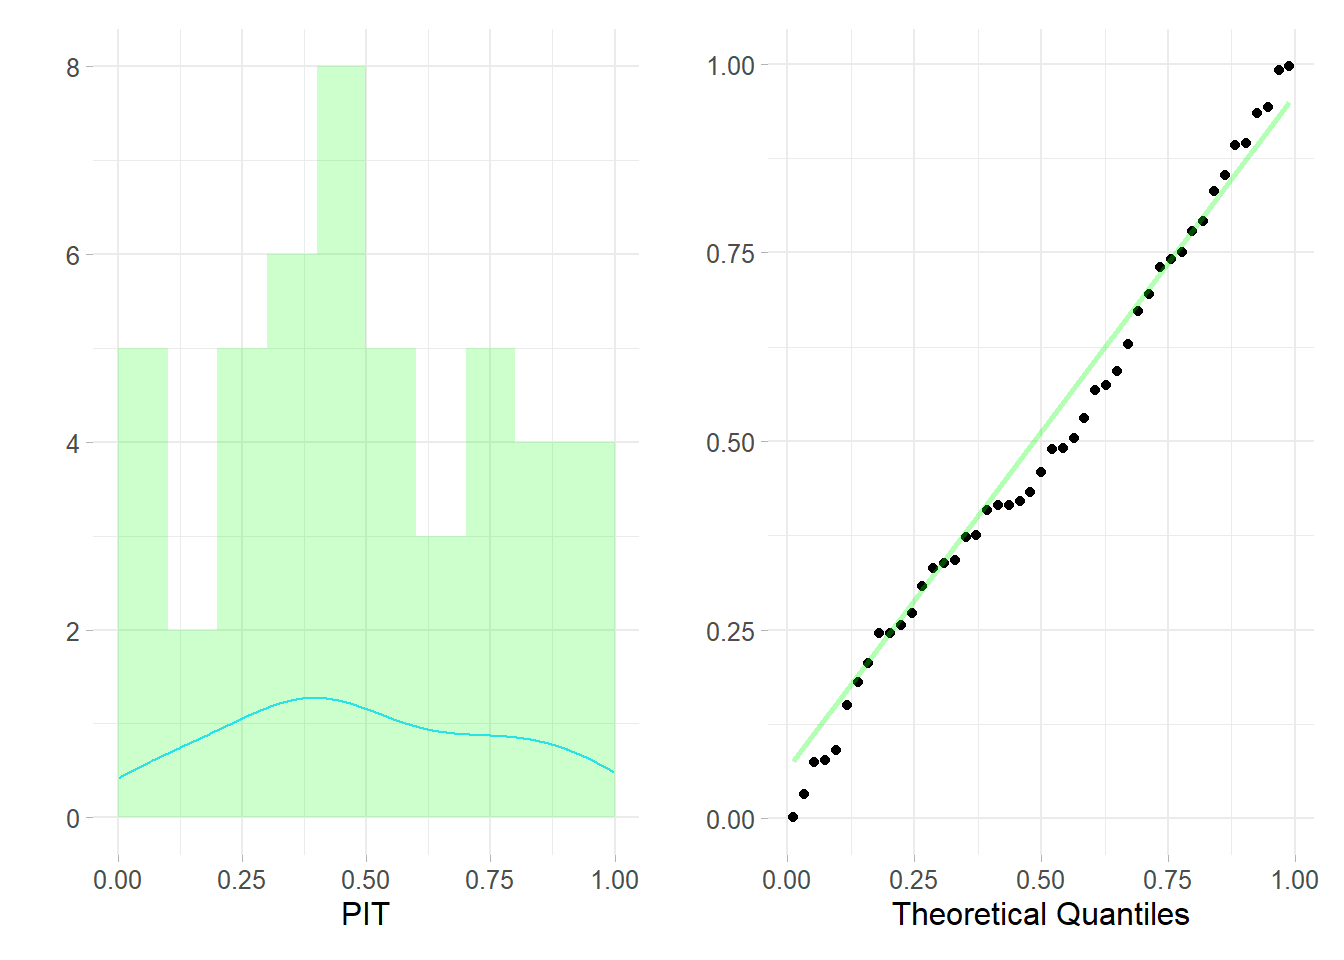
\includegraphics{05-prd_modelling_files/figure-latex/pitcpo-1} 

}

\caption{Left: histogram of cross-validated PIT, Right: QQ plot for Unif(0,1)}\label{fig:pitcpo}
\end{figure}

Posterior Predictive checking methods \citep{gelman1996posterior} exploit a full cross-validation where \(\boldsymbol{y}_{A} = \boldsymbol{y}_{V}\), operating on the full set of observation. The statistics capitalized below are quite commonly used in practice, but they are high context dependent:

\begin{itemize}
\tightlist
\item
  the \emph{posterior predictive distribution}: \(\pi(y^{\star} \mid \boldsymbol{y}) = \int \pi(y^{\star} \mid \theta_{i})\pi({\theta_{i}} \mid \boldsymbol{y})\mathrm{d}\theta_{i}\) which is the likelihood of a replicate observation. When values are small that indicates that are those values are coming from tails, since the area under the curve (i.e.~probability) is less. If this happens for many observation then outliers are driving the model leading to poor estimates
\item
  the \emph{posterior predictive p-value} whose math expression is:\(\pi(y^{\star} \leq y_{i} \mid \boldsymbol{y})\) for which values near to 0 and 1 indicates poor performances.
\item
  the \emph{Root Mean Square Predictive Error RMSE}: \(\sqrt{\frac{1}{n} \sum_{i=1}^{n}(y_{i}-{y}^{\star}_{i})^{2}}\)
\item
  \(R^2\)
\end{itemize}

R-INLA has already antiticipated in chapter 4 section\ref{example} have dedicated function to compute statistics on posterior distribution e.g.~\passthrough{\lstinline!inla.pmarginal()!} returning the cumulative density distribution.

\hypertarget{devbased}{%
\subsection{Deviance-based Criteria}\label{devbased}}

If there is an interest in comparing multiple models, then their deviance may be used. Given data \(\boldsymbol{y}\) and its likelihood function, along with its parameters \(\boldsymbol\theta\) then the \emph{deviance} is:

\[
\mathrm{D}(\theta)=-2 \log (\pi(\boldsymbol{y} \mid \theta))
\]

The model's deviance tests the likelihood variability conditioned to its parameters. Since this is a random variable tt can be analyzed by several statistics such as mean, median, mode etc. The most used is the posterior mean deviance i.e.\(\overrightarrow{\mathrm{D}}=E_{\theta_{\mid y}}(\mathrm{D}(\theta))\) which is also robust \citep{Blangiaro-Cameletti}. Indeed it suffers from cost complexity, as a result DIC proposed by \citet{spiegelhalter2002bayesian} adds to the deviance a penalization for complex model i.e.~\(p_{\mathrm{D}}=\mathrm{E}_{\theta_{\mathrm{y}}}(\mathrm{D}(\theta))-\mathrm{D}\left(\mathrm{E}_{\theta_{\mathrm{y}}}(\theta)\right)=\overline{\mathrm{D}}-\mathrm{D}(\bar{\theta})\) from which, following \citet{Blangiaro-Cameletti} obtain,

\begin{equation}
  \mathrm{DIC}=\overline{\mathrm{D}}+p_{\mathrm{D}}
\label{eq:dic}
\end{equation}

Data is best served in models with small-scale DICs and the correspondent INLA option setting is analogous to the ones seen sec.~\ref{predbase}. INLA moreover take advantage of the hierarchical structure and computes different posterior deviances for latent parameters i.e.~mean and hyper parameters i.e.~mode (due to skewness). For further discussions \citet{spiegelhalter2014deviance} oppose DIC with other criteria for model comparison. Finally the Watanabe Akaike information criterion (WAIC) which is more Bayesian orthodox in setting up the criteria, for this reason is also more preferred \citep{gelman2014understanding}.

\hypertarget{priorsspec}{%
\section{Penalized Complexity Priors}\label{priorsspec}}

The priors choice is the most central part of a Bayesian analysis and at the same time the weakest since any selection might be criticized. Priors expression involves a considerably high amount of subjectivity and domain experience which may be imported from other comparable literature works or results. However according to purists Bayesian priors should be decided \emph{a-priori}, without either looking at the data, nor the posterior results. This can be tedious since many models are sensitive to priors, as evidenced in the example in sec.~\ref{rinla}. Priors may negatively impact posteriors when are
wrong and they usually require a later revision. The choice in this context is also more difficult since it is also constrained to LGM requirements for which the latent field demands them to be jointly Gaussian.
\citet{simpson2017} provide a solid backbone knowledge on priors specification in Hierarchical models by setting up 4 guidelines principles on top of which it is built a new prior class called Penalized Complexity (PC) priors. Before jumping into the principles it is needed an abstract concept that goes by the name of ``base model''. For a general density \(\pi(\mathbf{y} \,| \,\xi)\) which is controlled by a flexibility parameter \(\xi\) the base model is the most uncomplicated one in the class. Following the notation this would be the model corresponding to \(\xi = 0\). The base model ideally grabs the parameter choice with the lowest possible complexity given the model and set it as a ground benchmark. The following example regards base model for a a Gaussian Random effect and it considers a multivarite gaussian distributed with mean \textbf{0} and precision matrix \(\tau \boldsymbol{Q}\), i.e.~\(\mathbf{y} \mid \xi \sim \operatorname{MVN}(\, 0\, ,\,\tau \boldsymbol{Q})\), where \(\tau=\xi^{-1}\). The base model tries to put the mass \citeyearpar{simpson2017} on \(\xi = 0\) since the base model in this case is a model without the random effect. At this point it is possible to present the building blocks, first priciple is \emph{Occam's razor} according to which priors should be weighted down in fuction of the distance between the added complexity and the base model i.e.~simpler models are preferred. The second principle regards how it is measured complexity whose solution is found in KLD (Kullback--Leibler divergence), calculating distance \(d\) from base model. KLD in this context along with principle 1 affirms that the prior shall have high mass in areas where replacing the base model with the flexible model will not cause any information loss. Principle 3 is constant rate penalization as names suggest relates the distance \(d\) to a constant rate penalization whose assumption implies an exponential prior on the distance scale, i.e.~\(\pi(d) = \lambda \exp (-\lambda d)\). In the end, the PC prior is described in the required scale with probability statements on the model parameters. Statement regards the selection of two further user defined (here the subjectivity) hyper-parameters, \(U\) regulating the tail event and \(\alpha\) the mass to put to this event such that \(\operatorname{P}(Q(\xi)>U)=\alpha\). A prior satisfying all the requirements is said Penalized in Complexity.
Priors of this class should be then derived with respect to the specific content they are needed. In this context PC priors are seen for Gaussian Random effect, i.e.~the GP \ref{def:GP} modeling spatial dependence for which a precision hyper parameter is demanded. The PC prior for the precision \(\tau\) is on standard deviation scale \(\sigma=\tau^{-1 / 2}\).\\
Then the GMRF latent field has mean 0 and covariance matrix \(\boldsymbol{Q^{-1}}\), i.e.~\(\boldsymbol{\theta} \sim \mathcal{N}\left(\mathbf{0}, \tau^{-1} \boldsymbol{Q}^{-1}\right)\). The base model considers the absence of the random effect which implies \(\tau \rightarrow \infty\). Then the derived PC prior \citep{simpson2017} takes the form of an exponential distribution, i.e.~``type-2 Gumbel distribution'' eq: \eqref{eq:exponential}, whose rate parameter is \(\lambda\) determining the severity of the penalty when diverging from the base model. Note that the parameter \(\lambda\) is on the standard deviation scale (in contrast to the Gamma on the precision seen in \ref{rinla}).

\begin{equation}
  \pi(\tau)=\frac{\lambda}{2} \tau^{-3 / 2} \exp \left(-\lambda \tau^{-1 / 2}\right), \tau>0
\label{eq:exponential}
\end{equation}

The distribution depends on a rate parameter \(\lambda\) that regulates the penalty according to the probability natural criterion \citep{slides} \(\operatorname{Prob}(\tau^{-\frac{1}{2}} > U)=\alpha\). \(U\) in this case is an upper limit for the standard deviation (being in the base model) and \(\alpha\) a small probability. The probability statement aforementioned implies the follwing realtion \(\lambda=-\ln (\alpha) / U\). Some further investigations of \citet{simpson2017} acknowledged that parameters upper bounds for \(\tau\) are \(U = 0.968\), and \(\alpha = 0.01\), where alpha regulates the importance of the prior believe. Ideally it would be picked up \(U\) drawing on previous experience. Indeed a reasonable choice in the absence of knowledge might be taking the semivariogram range \ref{GP}, i.e.~where the spatial dependece disappears.
PC priors are natively implemented in INLA and are shown to be well suited for the modular additive definition \citep{Bayesian_INLA_Rubio}. As a consequence they are selected as prior candidates with a reasonable \(U\) selection and no sensitivity analysis is performed i.e.~evalutaing posterior disstribution while prior are changing.

Fig. \ref{fig:priorfun} indicates various PC priors using several \(\alpha\) values for the precision \(\tau\). Note that increasing \(\alpha\)'s values contribute to a stronger prior belief for \(U\) which then leads to a higher conviction of \(\tau\).

\begin{figure}

{\centering 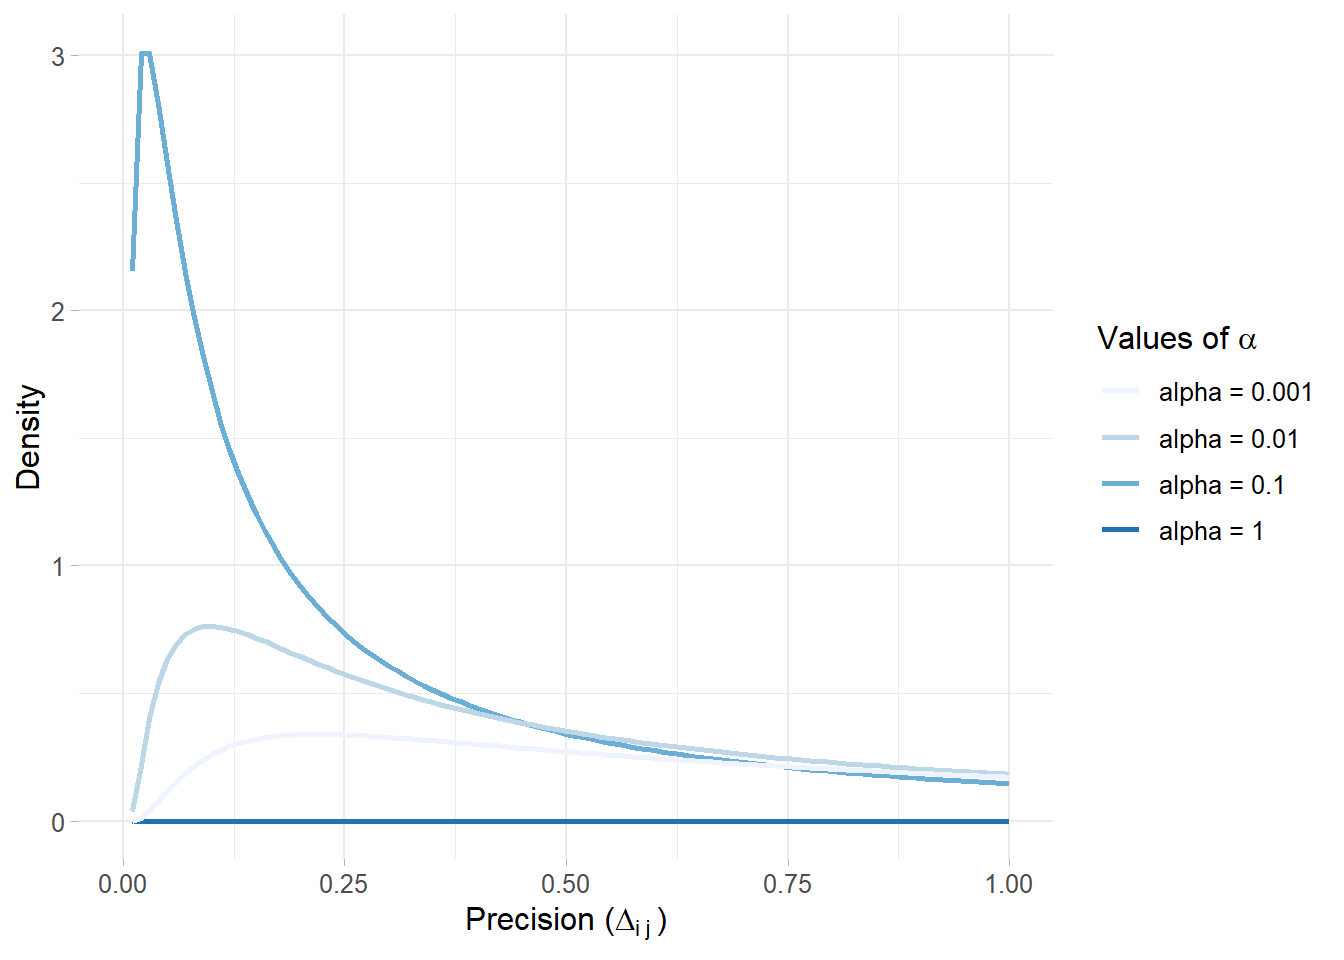
\includegraphics{05-prd_modelling_files/figure-latex/priorfun-1} 

}

\caption{PC priors for the precision by varying alpha values and fixing $U$}\label{fig:priorfun}
\end{figure}

\hypertarget{exploratory}{%
\chapter{Exploratory Analysis}\label{exploratory}}

To the analysis extent data should be constrained to the same geographic area and then saved otherwise the analysis would not be neither comparable nor reproducible since each time the API is called data gets updated. As a consequence the API is invoked with fixed request parameters by securing to the API the \passthrough{\lstinline!.thesis!} option, section \ref{docs}. In other words the (mandatory) argument option guarantees to specify to the API an already pre-composed url to be passed to the scraping endpoint. The choice for this analysis is submitting the url corresponds to the properties restricted to a fixed set of micro-zones inside the \emph{circonvallazione} i.e.~beltway of Milan ( \emph{Municipality of Milan} ). On the other side the resulting data is locally stored to be able to have consistent inference. (api parameters, number of covariates and number of observations)
Data emerging from the RESTful API response is not in its tidiest format. Yet data undergoes to a series of pre-processing steps during scraping, after which still requires to clear up unnecessary character and to separate columns containing more than one information. Therefore a summary table of the covariates, tab. \ref{tab:covartable}, involved into the analysis is presented with the goal to familiarize with incoming API data. Data gathered from the second \passthrough{\lstinline!/completescrape!} endpoint contains geostatistical components and consequently a map representation of Real Estate rental maket at the gitbook building time i.e.~2021-02-15 is given. A further plot assess spatial dependence highlighting that coordinates are non-linearly related \ref{fig:NonLinearSpatialRel} to the y-response monthlyprice variable. Exploration starts with factor counts evidencing a ``Bilocale'' prevalence. This implies some critical Milan real estate market demand information and consequently reflections on the offer. Data displays bimodality in prices distribution for different n-roomed accommodations and the model should take account of the behavior. Then a piece-wise linear regression is fitted for each household type accommodation factor, whose single predictor is the square meter footage. The analysis emphasize some valuable economic consequences both for investors interested into property expansions and for tenants that are planning to partition single properties into rentable sub-units. The previous analysis brings along a major question which addresses the most valuable properties per single square meter surface and an answer based on data is given. Then a log-linear model is fitted on some presumably important covariates to evaluate each single house characteristic contribution to the price. A Tie Fighter plot displays for which coefficient, associated to each dummy predictor, are encountered surprisingly high monthly prices, compared to the effect of the square meter footage expansion. A partial conclusion is that disposing of 2 or 3+ bathrooms truly pays back an extra monthly return, also due to the number of tentants the accomodations could host. Text mining techniques are applied on real estate agency reviews and a network graph can help to distinguish topics. Then Missing assessement and imputation takes place. At first is made a brief a revision on randomness in missing by \citet{Little} which may help to figure out if data is missing due to API failures or for other reasons. Theory is applied by visualizing missingness in combination with heat-map and co-occurrence plot. Combined missing observation test is able to detect whether data is missing because of inner scraping faiilures or simple low prevalence in appereance. Then for each of the covariate that pass the exam, then imputation is made through INLA posterior expectation. This is the case of missing data in predictors, so the missing covariates ( \emph{condominium} ) are brought into a model as response variable where this time predictors are the explanatory ones. Through a method specified within the INLA function the posterior statistics are computed and then finally imputed in the place of missing ones.

\begin{longtable}[t]{ll}
\caption{\label{tab:covartable}Covariates extracted on a general API call}\\
\toprule
name & descrition\\
\midrule
id & ID of the apartements\\
lat & latitude coordinate\\
long & longitude coordinate\\
location & property address: street name and eventual number\\
condom & condominium monthly expenses\\
\addlinespace
buildage & age in which the building was contructed\\
indivsapt & indipendent property type versus apartement type\\
locali & type and number of rooms\\
propcat & property category\\
status & maintenance status of the house, ristrutturato, nuovo, abitabile\\
\addlinespace
heating & heating system\\
ac & air conditioning\\
catastinfo & land registry information\\
aptchar & apartement characteristics\\
photosnum & number of photos displayed in the advertisement\\
\addlinespace
age & real estate agency name\\
enclass & energy class\\
contr & contract type proposed\\
disp & availability or already rented\\
totpiani & total number of building floors\\
\addlinespace
postauto & number of parking box or garages\\
review & estate agency review (long chr string)\\
total\_main\_surface & total apartement surface area\\
total\_commercial\_surface & total commercial surface area\\
constitution & covered and uncovered surface areas type\\
\addlinespace
floor & the property floor for each covered and uncovered area\\
surface & square meter footage for each covered and uncovered type\\
percentage & contribution percentage for each element to the total surface\\
surface\_type & appliances or princpal category surface\\
commercial\_surface & square meter footage for each commercial surface area\\
\addlinespace
multi & it if has multimedia option, (3D house ristualization home experience and videos)\\
original\_price & If the price is lowered it flags the starting price\\
current\_price & If the price is lowered it flags the current price\\
passed\_days & If the price is lowered marks the number of days passed by since the price change\\
date & the date of publication of the advertisement\\
\addlinespace
nroom & number of rooms (int)\\
price & monthly price € (response)\\
sqfeet & total square meters footage surface area (int)\\
title & title of advertisement\\
\bottomrule
\end{longtable}

\hypertarget{prep}{%
\section{Preprocessing and Feature Engineering}\label{prep}}

Data needs to undergo to many previous cleaning preprocess steps, which mainly regard separating columns and extracting relevant covariates. This is a forced stage since for the way the API is designed it tries several searches (refer to fig.~\ref{fig:pseudocode1}). Chances are that the search algorithm explores a hidden json object nested in the website source code, which actually needs to be properly wrangled. Steps followed are:

\begin{itemize}
\tightlist
\item
  \emph{locali} needs to be separated, from which are drained out 5 categories : \emph{totlocali}, \emph{camereletto}, \emph{altro}, \emph{bagno}, \emph{cucina}. \emph{nroom} now is a duplicate for \emph{totlocali}, so it is discarded.
\item
  \emph{aptchar} is a character string column that contains a non fixed number of features per house. The preprocess steps include cleaning the string from unnecessary characters, finding the set of unique elements across the character column (regex pattern), separating each feature in its proper column, in the end recoding newly created bivariate columns as ``yes'' or ``no'' according to a matching pattern.
\item
  dropped unnecessary non UTF characters from continuous integer covariates i.e.~\emph{price}, \emph{condominium}, \emph{sqfeet}
\item
  recoded factors for \emph{totlocali} and \emph{floor}
\end{itemize}

The previous steps lead to have a 250 data points per 64 covariates. Ultimately exploiting the spatial component, data can be represented through a map, as in fig.~\ref{fig:LeafletVisuals}. Maps (not properly a ``spatial'' visualization) must determine the regularity of the arrangement of points and also if the maximum gap between points is much greater in some directions than others (symptomps of anisotropy, not detected).

\begin{figure}

{\centering 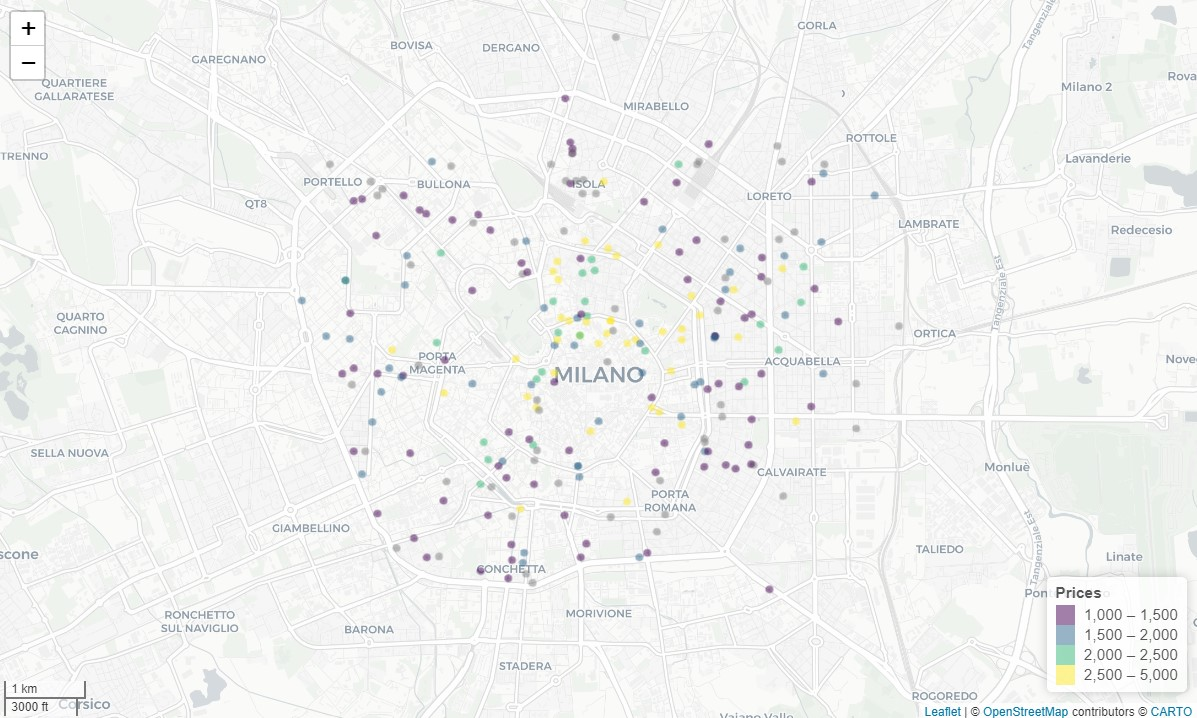
\includegraphics[width=1\linewidth]{images/leaflet_prezzi} 

}

\caption{Leaflet Map}\label{fig:LeafletVisuals}
\end{figure}

\hypertarget{spatassess}{%
\section{Spatial Dependece Assessement}\label{spatassess}}

Spatial continuous data, as Waldo Tobler's first law suggests, may be split split into a mean term and an error term \citep{Banerjee-Gelfand}. The mean is the global (or first order) behaviour, while the error reports a contextual (or second-order) behavior through a covariance function. An effective set of EDA on spatial data should be able to separate and correctly detect these two quantities. As a matter of fact spatial data association for the spatial process \(Y(s)\) need not imitate its residuals \(\epsilon(s)\). A 3D scatterplot elevated for the price is plotted in \ref{fig:3dmap}, this is effective in displaying how the response is spatially dependent however it does not reveal the entire spatial surface. Moreover it can be tricky since it can display a spatial pattern that vanishes as soon as a model is fitted or vice versa. The analysis of spatial variations in the residual seems more organic \citeyearpar{Banerjee-Gelfand}

\begin{figure}
\centering
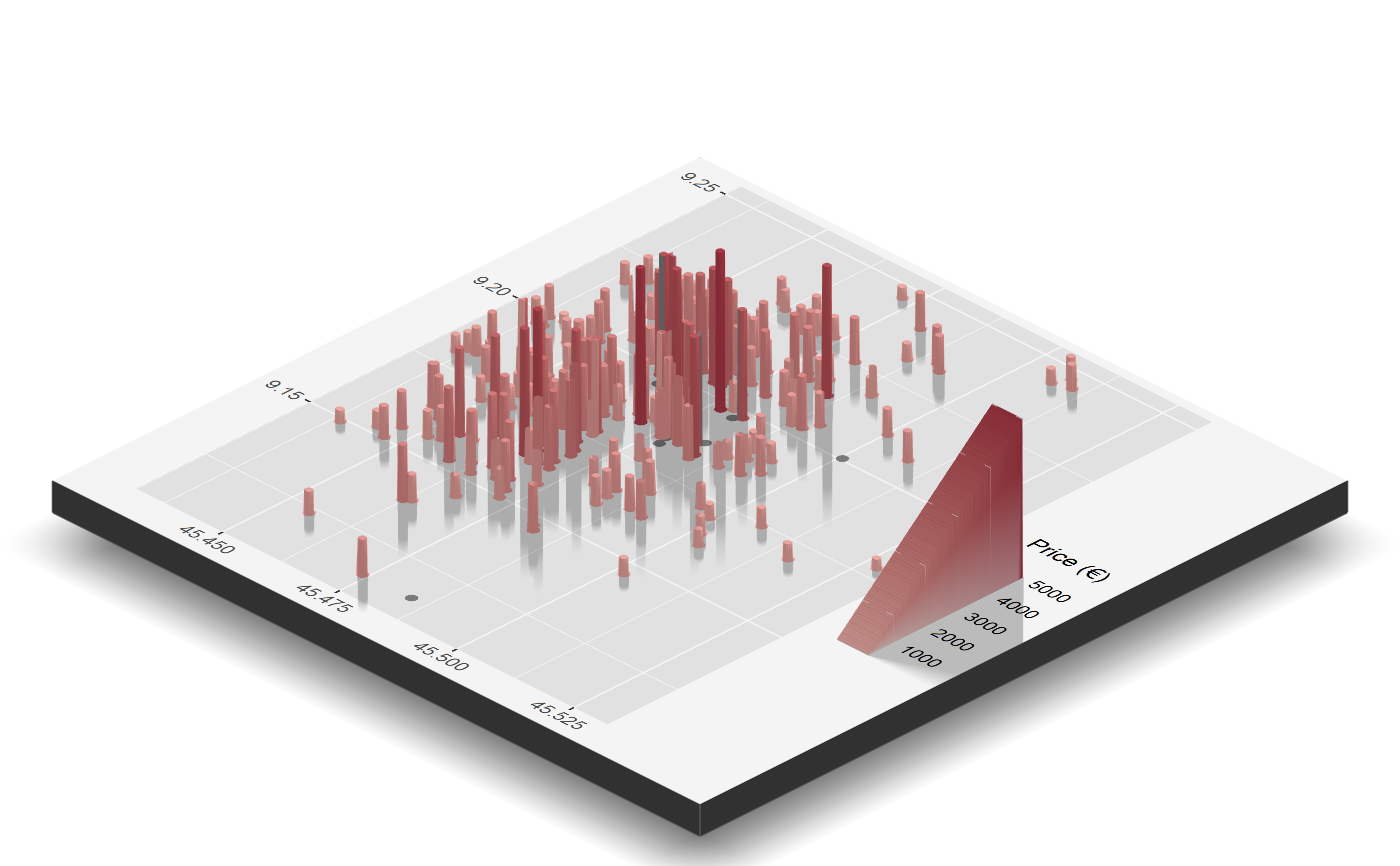
\includegraphics{images/3d_map2.png}
\caption{\label{fig:3dmap}3D Rayshader \citet{rayshader} Perspective scatterplot with Price elevation}
\end{figure}

By visual inspection, even though is assumed, the distribution of price seems to suffer for spatial dependence. In order to measure the range of spatial dependency and get an idea about the sill and nugget (seen in section \ref{GP} of previous chapter), further research is urged through a variogram analysis. The assessment continues by fitting an isotropical semivariogram with Matérn covariance \ref{fig:matern} on residuals due to the assumption made before. Residuals are extracted from a regression model whose formula relates price with other presumably important covariates i.e.~\(\text{price} \sim \text{totlocali} + \text{condominium}+ \text{sqmeter}\). The model is also computed through inla and by taking advantage of \passthrough{\lstinline!INLAtools!} and Pearson residuals \citep{pearson} are extracted, i.e.~\(\operatorname{Pearson}_{i}=\frac{y_{i}-\hat{y}_{i}}{\sqrt{M S E}}\). Moreover variogram from package \passthrough{\lstinline!gstat!} is versatile enough to allow to specify a regression model within the variogram function. The range parameter initial value is set equal to the maximum pair points distance registered.

\begin{figure}

{\centering 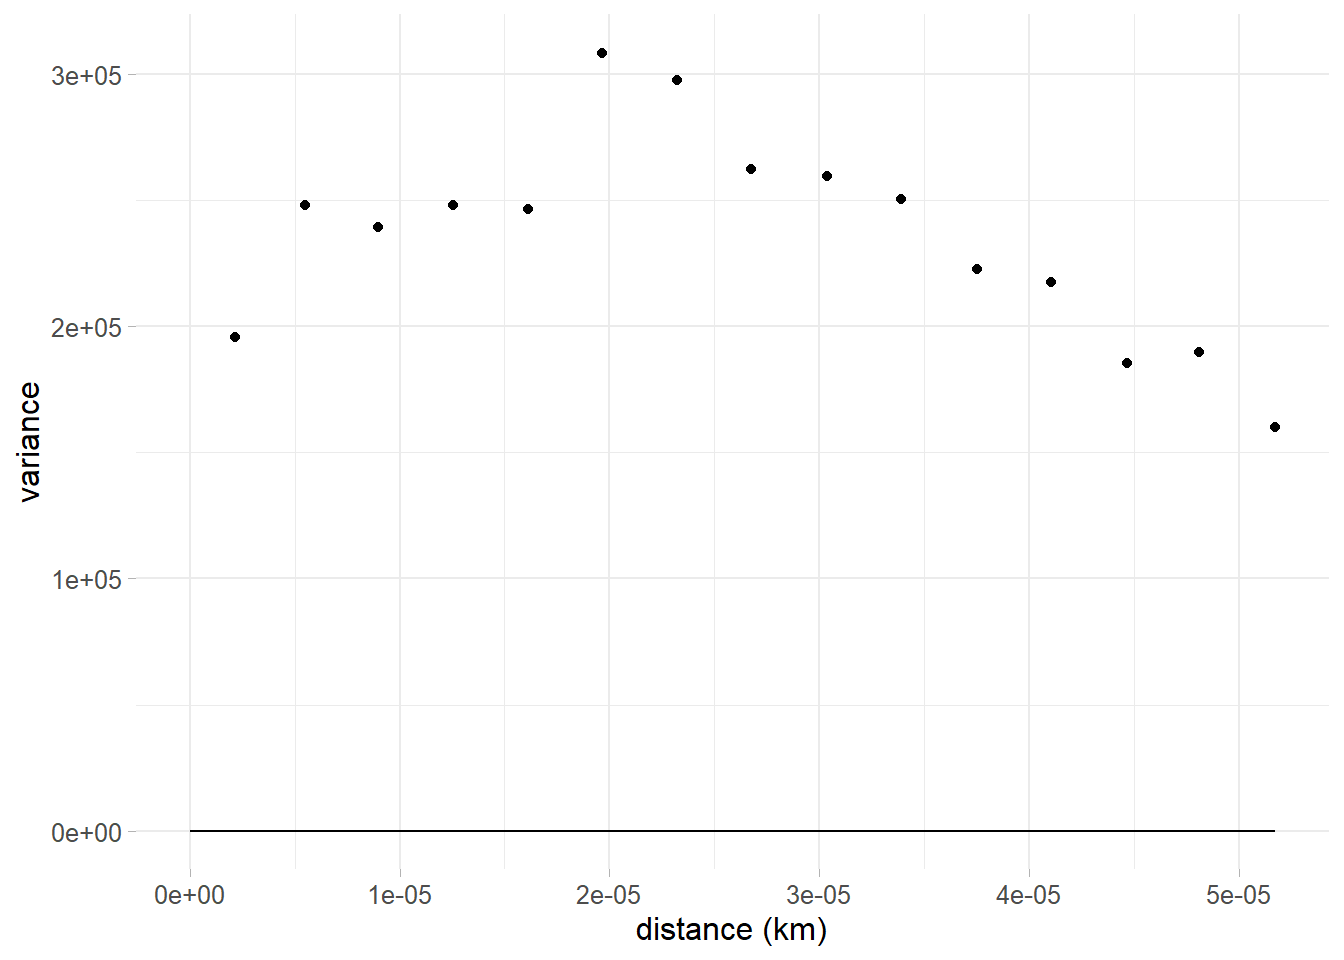
\includegraphics{06-exploratory_files/figure-latex/semivariogram-1} 

}

\caption{Semivariogram on a linear model Pearson residuals}\label{fig:semivariogram}
\end{figure}

\hypertarget{factor-counts}{%
\section{Factor Counts}\label{factor-counts}}

Arranged Counts for categorical columns can give a sense of the distribution of categories across the dataset suggesting also which predictors and which factor is relevant to the analysis. The left panel in figure \ref{fig:fctCounts} offers the rearranged factor count fot the covariate \emph{TOTLOCALI}. ``Bilocale'' are the most common option for rent, then ``Trilocale'' follows. The intuition behind suggests that Milan rental market is oriented to ``lighter'' accommodations in terms of space and squarefootage. This comes natural since Milan is both a vivid study and working area, so temporary accommodations are warmly welcomed. Right in figure \ref{fig:fctCounts} it can be seen that building are generally old and mostly built either at the start of the 20th century or in the middle. Further investigation might assess how this fact can affect the overall city status.

\begin{figure}

{\centering 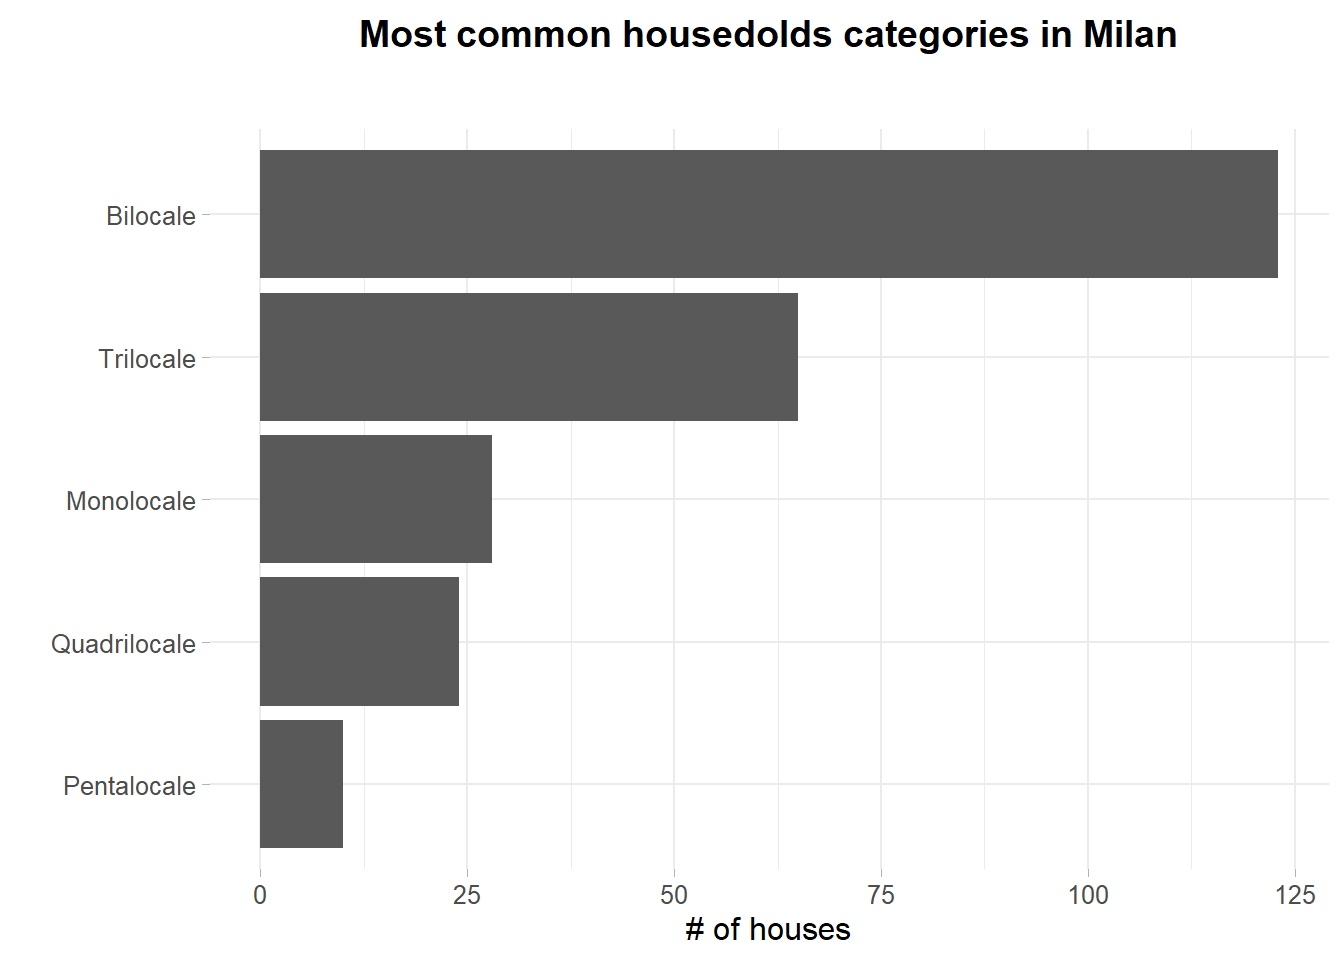
\includegraphics{06-exploratory_files/figure-latex/fctCounts-1} 

}

\caption{Left: Count plot for each housedolds category, Right: count plot for building age}\label{fig:fctCounts}
\end{figure}

Two of the most requested features for comfort and livability in rents are the heating/cooling systems. Moreover rental market demand, regardless of the rent duration, strives for a ready-to-accomodate offer to meet clients expectation. In this sense accommodation coming with the newest and the most technologically advanced systems are naturally preferred.
x-axis in figure \ref{fig:PricePerAc} represents \(\log_{10}\) price for both of the upper and lower panel. Logarithmic scale is needed to smooth distributions and the resulting price interpretation have to considered into relative percent changes. Furthermore factors are reordered with respect to decreasing price.\\
y-axis are the different level for the categorical variables recoded from the original data due to simplify lables and to hold plot dimension. Moreover counts per level are expressed between brackets close to their respective factor.
The top plot displays the most prevalent heating systems categories, among which the most prevalent is ``Cen\_Rad\_Met'' by far. This fact is extremely important since methane is a green energy source and if the adoption is wide spread and pipelines are well organized than the city turns out to be sustainable. Indeed according to data there is still a 15\% portion of houses powered by oil fired (old and polluting heating systems), which has been already presumed in the previous plot. This partially explains why Milan is one of the most polluted city in the world.
Then in bottom plot Jitters point out the number of outliers outside the IQR (Inter Quantile Range) .25 and their impact on the distribution. A first conclusion is that outliers are mainly located in autonomous systems, which leads of course to believe that the most expensive houses are heated by autonomoius heating systems. Indeed in any case this fact that does not affect monthly price. The overlapping IQR signifies that the covariates levels do not impact the response variable.

\begin{figure}

{\centering 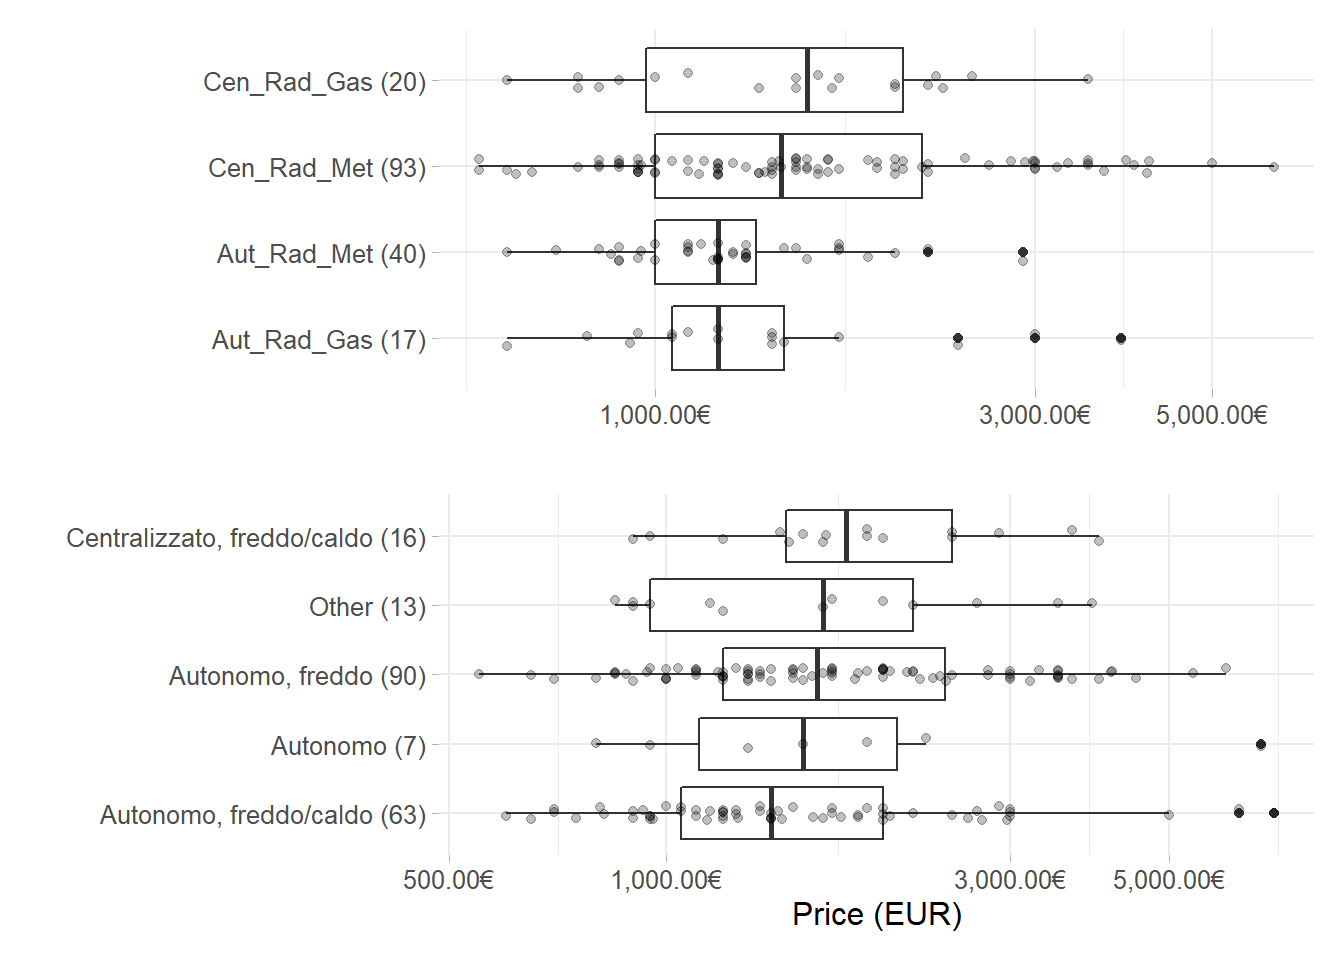
\includegraphics{06-exploratory_files/figure-latex/PricePerAc-1} 

}

\caption{Log Monthly Prices box-plots for the most common factor levels in Heating systems and Air Conditionings}\label{fig:PricePerAc}
\end{figure}

\hypertarget{mvp}{%
\section{Assessing the most valuable properties}\label{mvp}}

It might be relevant also to research how monthly prices change with respect to houses' square footage for each house configuration, in other word how much adding a further square meter affects monthly price for each n-roomed flat.
Answering to the previous question implies also knowing how properties should be developed in order to request a greater amount of money per month. This may be of interest, for instance, to those who have to lot their property into sub units and need to decide the most profitable choice in economic terms by setting \emph{ex ante} the square footage extensions.
A further example may regard the economic convenience for those who need to enlarge new properties (construction firms). Some of the potential enlargements are economically justified, some of the other are not.
The plot \ref{fig:GlmPriceSq} has two continuous variables for x (price) and y (sqfeet) axis, the former is once again \(log_{10}\) scaled. Coloration discretizes points for each of \(j_{th}\) totlocali. A sort of overlapping piece-wise linear regression (log-linear due to the transformation) is fitted on each totlocali group, whose response variable is price and whose only predictor is the square footage surface (i.e.~\(\log_{10}(\text{price}_j) \sim +\beta_{0,j}+\beta_{1,j}\, \text{sqfeet}_j\)). Five different regression models are proposed in the top left. The interesting part regards the models slopes \(\hat\beta_{1,j}\). The highest corresponds to ``Monolocale'' for which the enlargement of a 10 square meters in surface enriches the apartment of a 0.1819524\% monthly price addition. Almost the same is witnessed in ``Bilocale'' for which a 10 square meters extension gains a 0.1194379\% value. One more major thing to notice is the ``ensamble'' regression line obtained as the interpolation of the 6 plotted ones. The line suggests a clear logarithmic pattern from Pentalocale and beyond whose assumption is strengthened by looking at the decreasing trend in the \(\hat\beta_1\) predictor slopes coefficients. Furthermore investing into an extension for ``Quadrilocale'' and ``Trilocale'' is \emph{coeteris paribus} an interchangeable economic choice.

\begin{figure}

{\centering 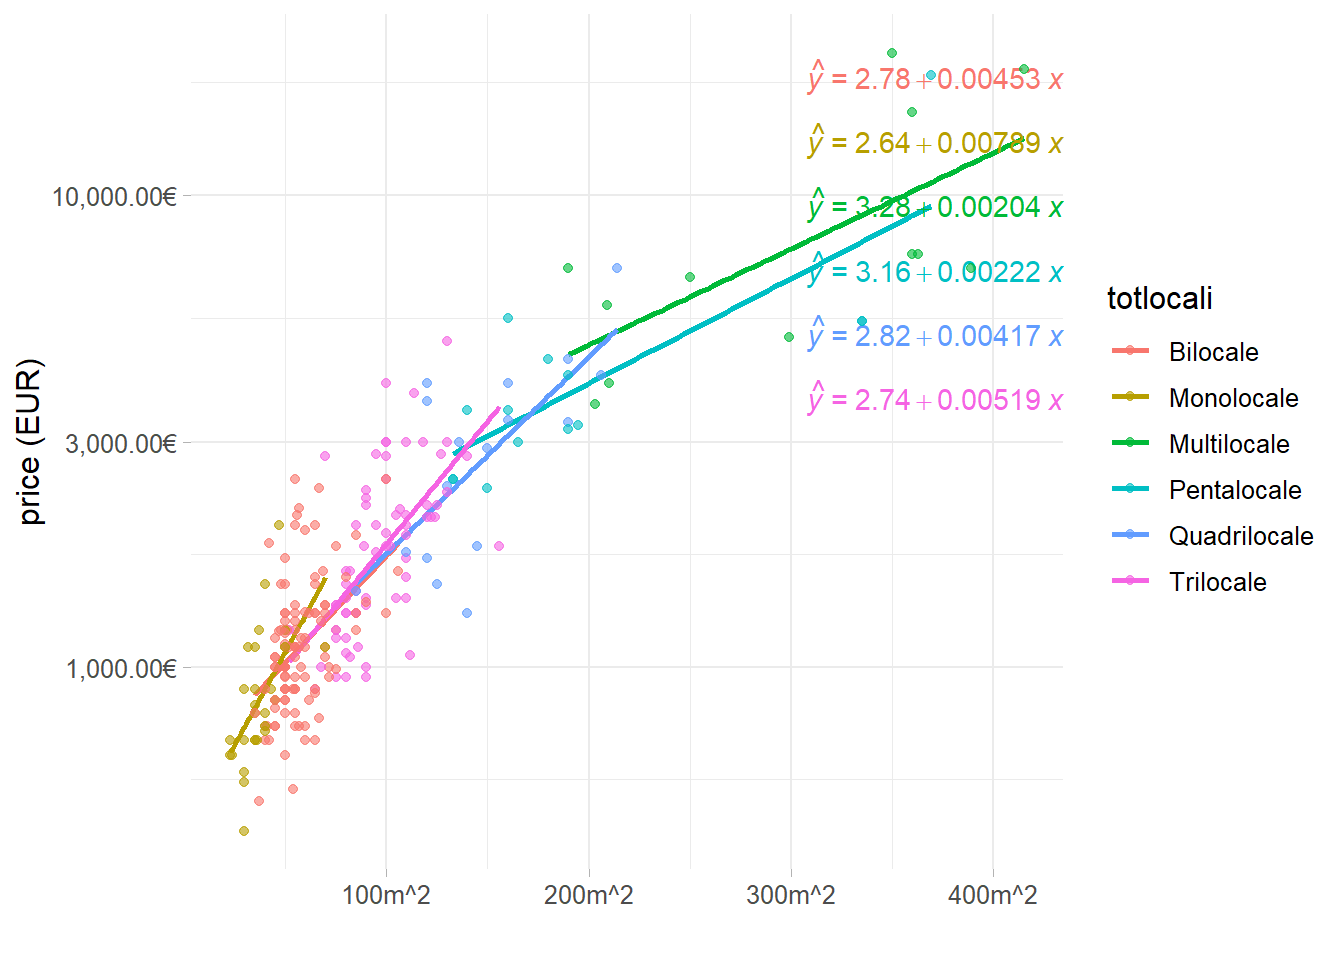
\includegraphics{06-exploratory_files/figure-latex/GlmPriceSq-1} 

}

\caption{Monthly Prices change wrt square meters footage in different n-roomed apt}\label{fig:GlmPriceSq}
\end{figure}

Furthermore in table \ref{tab:TopAbsPrice} resides the answer to the question ``which are the most profitable properties per square meter footage''. The covariate floor together with the address are not part of this simple regression model, indeed they can help explaining the behavior. First and third position are unsurprisingly ``Bilocale''. The second stands out for its ridiculous price per month. The other are all located nearby the city center.

\begin{table}

\caption{\label{tab:TopAbsPrice}The most profitable properties per single square meter footage at the date of2021-02-15}
\centering
\begin{tabular}[t]{llrrlll}
\toprule
location & totlocali & price & sqfeet & floor & totpiani & abs\_price\\
\midrule
via della spiga 23 & Bilocale & 2500 & 55 & 2 & 4 piani & 45.45€\\
via dei giardini C.A. & Multilocale & 18500 & 415 & 2 & 6 piani & 44.58€\\
piazza san babila C.A. & Bilocale & 1833 & 42 & 1 & 4 piani & 43.64€\\
ottimo stato nono piano, C.A. & Monolocale & 2000 & 47 & 9 & 11 piani & 42.55€\\
via tommaso salvini 1 & Multilocale & 15000 & 360 & 5 & 6 piani & 41.67€\\
\addlinespace
via cappuccini C.A. & Trilocale & 4000 & 100 & 3 & 5 piani & 40€\\
\bottomrule
\end{tabular}
\end{table}

\hypertarget{assessing-relevant-predictors}{%
\section{Assessing relevant predictors}\label{assessing-relevant-predictors}}

Now it is fitted a log-linear model whose response is price and whose covariates are the newly created abs\_price and some other presumably important ones e.g.~floor, bagno, totpiani. The model formula is \(\log_{2}(price) \sim \log_{2}(abs\_price) + condominium + other_colors\).
The plot in figure \ref{fig:TieFighterPlot} has the purpose to demonstrate how monthly price is affected by covariates conditioned to their respective square meter footage. The interpretation of the plot starts by fixing a focus point on 0, which is the null effect highlighted by the red dashed line. Then the second focus is on house surface effect (i.e.~House Surface (doubling) in the plot, the term \(\log_{2}(abs\_price)\) has been converted to more familiar House Surface (doubling)), which contributes to increase the price of an estimated coefficient of \(\approx .6\) for each doubling of the square meter footage. Then what it can be noticed with respect to the two focus points are the unusual effects provoked by the other predictors to the right of the doubling effect and to the far left below 0. ``2 bagni'', 3 bagni" and 3+ bagni" are unusually expensive with respect to the square meter footage increment, on the other hand ``al piano rialzato'' and ``al piano terra'' are undervalued with respect to their surface. The fact that 2 and 3 bathrooms can guarantee a monthly extra check is probably caused to a minimum rent plateau requested for each occupant. the number of bathrooms are a proxy to both house extension since normally for each sleeping room there also exist at least 1 bathroom as well as prestigious houses dispose of more than 1 toilette services. So the more are the occupants regardless of the square meter footage dedicated to them, the more the house monthly returns.

\begin{figure}

{\centering 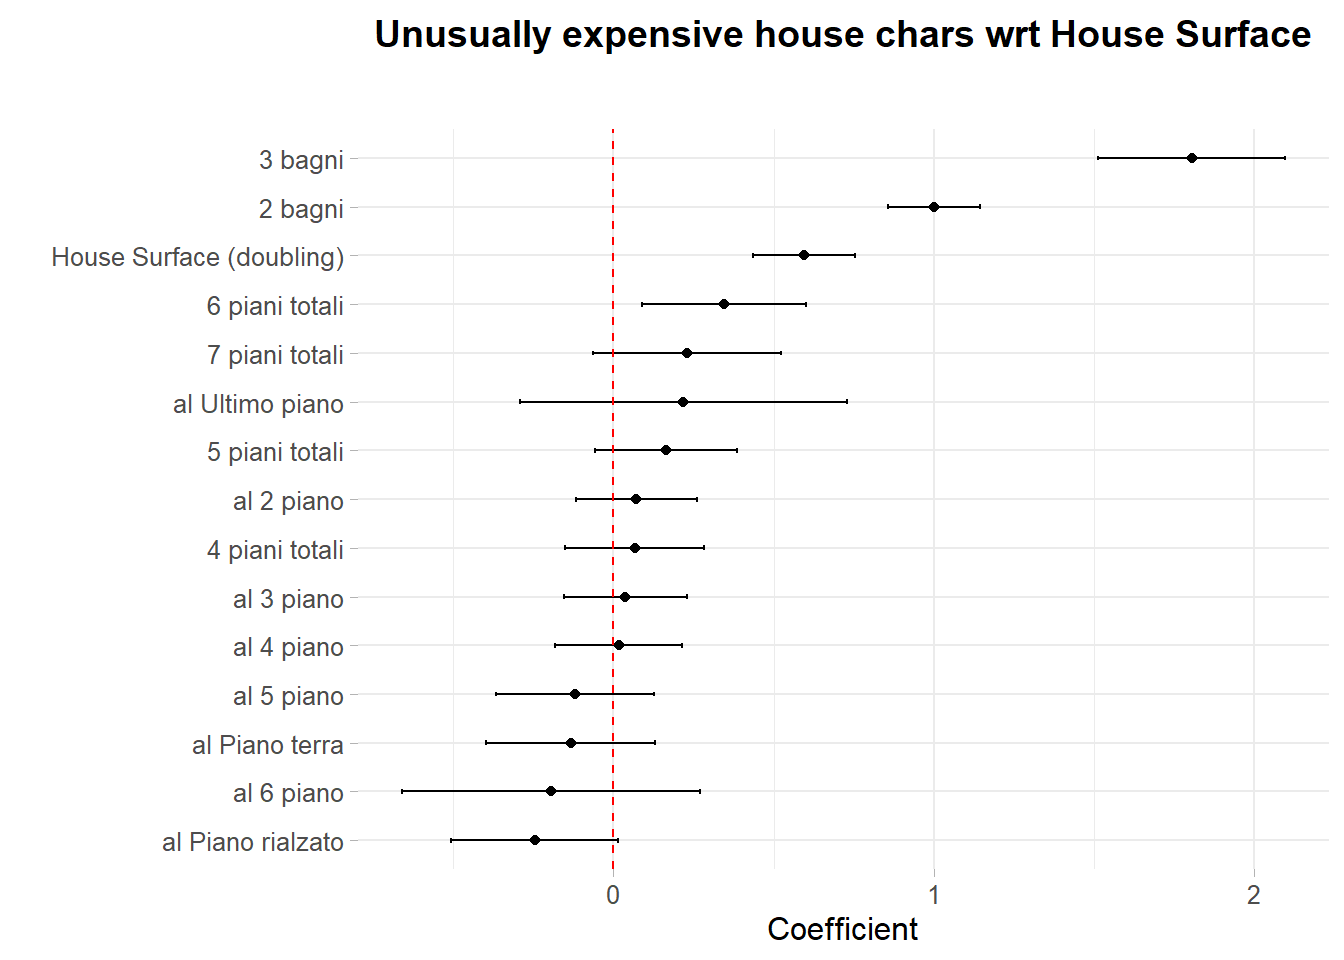
\includegraphics{06-exploratory_files/figure-latex/TieFighterPlot-1} 

}

\caption{Tie fighter coefficient plot for the log-linear model}\label{fig:TieFighterPlot}
\end{figure}

\hypertarget{missassimp}{%
\section{Missing Assessement and Imputation}\label{missassimp}}

Some data might be lost since immobiliare provides the information that in turn are pre filled by estate agencies or privates through standard document formats. Some of the missing can be traced back to scraping, some other are due to the context. The section tries to give substantial insights to discern what it can be recalled to the former issue or to the latter. The guidelines followed in this part is to prune redundant data and rare predictors trying to limit the dimensionality of the dataset as well as keeping covariates that are assumed to be relevant.

\hypertarget{missing-assessement}{%
\subsection{Missing Assessement}\label{missing-assessement}}

When data is presenting missing values, the analyst should typically investigate the etiology its lack \citep{Kuhn}. As already pointed out in the dedicated section \ref{ProperScraping} many of the presumably important covariates (i.e.~price lat, long, title ,id \ldots) undergo to a sequence of nested searches within the web page with the aim to avoid to be lost. This guarantees that when data is missing is actually due to an improper advertisement completion when posting the offer and by no means to a superficial scrape. Moreover empirical observation suggests that when relevant advertisement data is absent then it is more likely that the rest of the information are missing too.
However in the API context the missing profile is crucial since it can also raise suspicion on scraping inability to catch data. By taking advantage of the patterns the maintainer can directly identify which data or combination of data are missing and immediately debug the error. In order to identify the nature of the missing patterns a revision of missing and randomness is introduced \citep{Little}.
Categories are three:

\begin{itemize}
\tightlist
\item
  \emph{MCAR} (Missing Completely At Random ), the likelihood of missing is equal for all the information, in other words missing data are one independent from the other.
\item
  \emph{MAR} (Missing At Random). the likelihood of missing is not equal.
\item
  \emph{NMAR} (Not Missing At Random), data that is missing due to a specific cause, scarping is an option.
\end{itemize}

This MNAR case is difficult to detect since the missing process and details are not available. An example of MNAR is the case of daily monitoring clinical studies \citeyearpar{Kuhn}, when patient might drop out the experiment because of death, as a result all the subsequent data starting from the death time +1 are lost.
Patterns are visible through a statistical tool whose typical application is found in detecting collinearity in predictors i.e.~\emph{heat map}. The plot in fig.~\ref{fig:Heatmap} assign \(1\) when data is present and \(0\) otherwise. Gray background signifies data presence, black absence.

\begin{figure}

{\centering 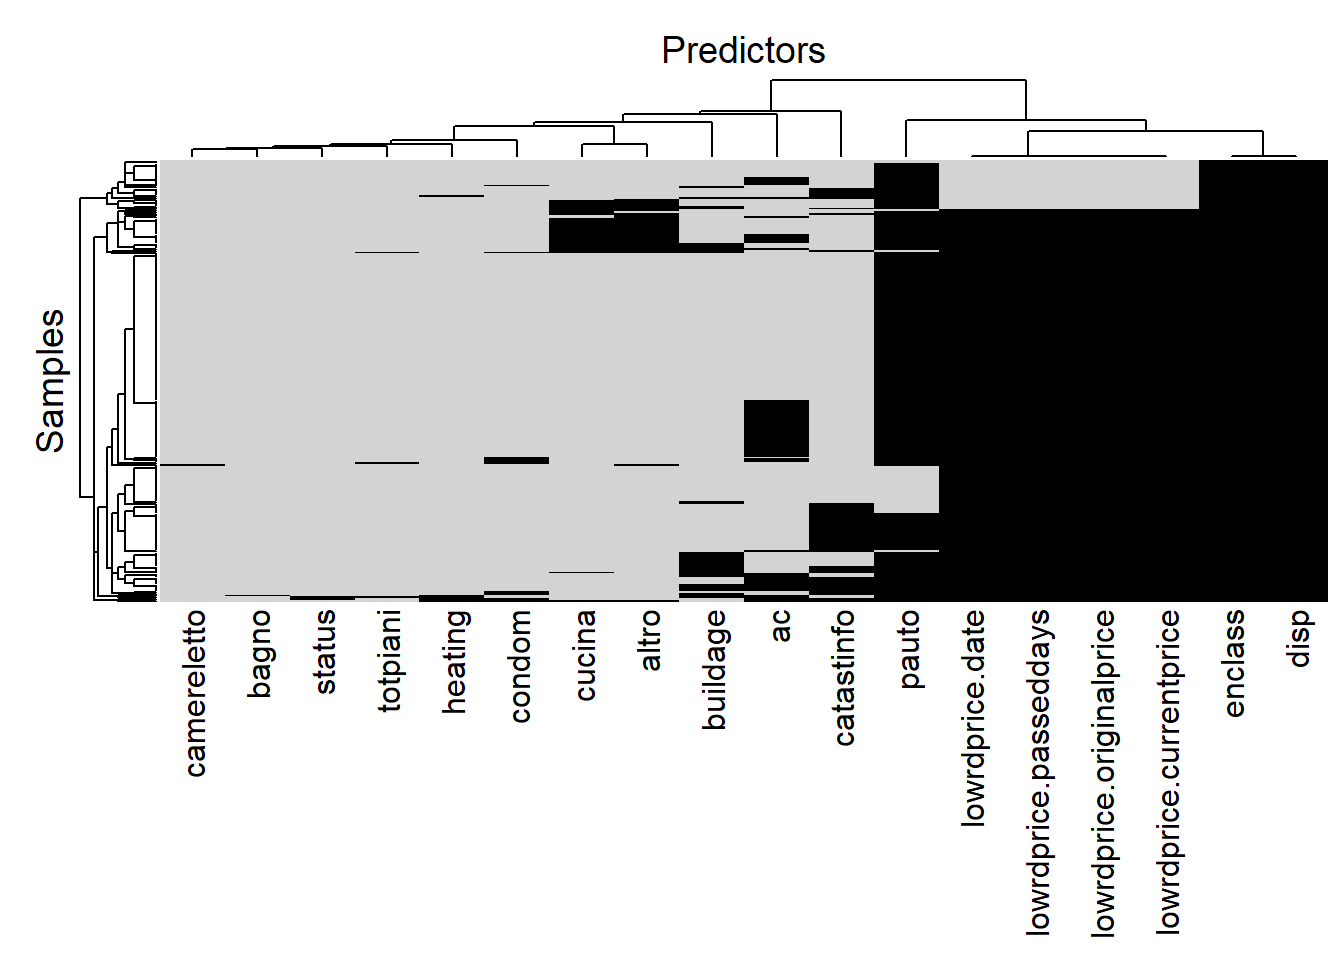
\includegraphics{06-exploratory_files/figure-latex/Heatmap-1} 

}

\caption{Heatmap of missing observations where gray implies data presence otherwise black, author's source}\label{fig:Heatmap}
\end{figure}

Looking at the top of the heat map plot, the first tree split divides predictors into two sub-trees. The left branch considers from \emph{camereletto} to \emph{ac} and there are no evident patterns except for a small portion of the group from \emph{constitution} to \emph{commercial surface}. In the former group the missing pattern can be traced back to MAR and covariate imputation for \emph{condom}, \emph{photosnum} and \emph{price} is scheduled (response and relevant continuous covariate). In the latter group a further inspection in the scraping code suggests that missing pattern are traced back to an improperly parsed json object in the source code, that is the case of NMAR and observations needs to be left out (covariate are not assumed to be important, therefore are not included in the model). From \emph{cucina} to \emph{post\_auto} a relevant pattern is evident for \emph{cucina} and \emph{altro}, that is because they come from the same predictor from which have been feature engineered two separated and different covariates. As a result the observations that are missing for the one are also missing for the other. Nonetheless the entire group of covariates is dropped due to rarity (percentages of missing are found in tab. \ref{tab:}).
In the far right side of figure \ref{fig:Heatmap} \emph{enclass}, \emph{catastinfo} and \emph{disp} data are completely missing (NMAR), the pattern suggests some problem in gathering the respective values. A further assessement of the API totally absent covariates scraping is strongly advised. From \emph{total\_commercial\_surface} to \emph{date}, as in cooccurrence plot in figure \ref{fig:cooccurrence}, they are missing in combination for a total of 196 out of 250 cases, therefore are dropped, even though the pattern is NMAR, suggesting that are strongly tied in the scraping process.

\begin{figure}

{\centering 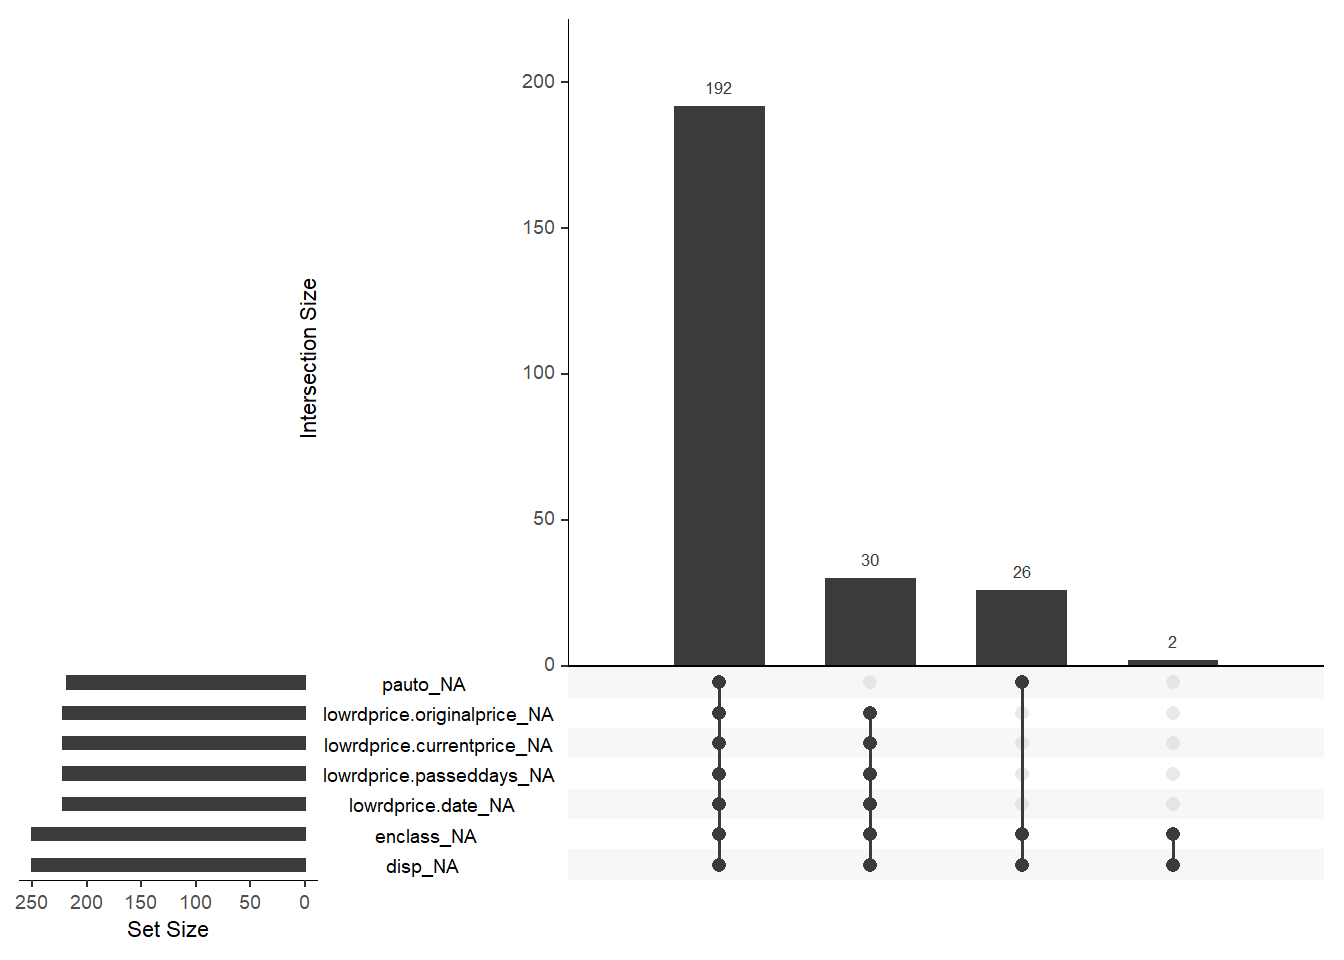
\includegraphics{06-exploratory_files/figure-latex/cooccurrence-1} 

}

\caption{Missingness co-occurrence plot}\label{fig:cooccurrence}
\end{figure}

\hypertarget{missing-imputation}{%
\subsection{Missing Imputation}\label{missing-imputation}}

A relatively simple approach to front MAR is to build a regression model to explain the covariates that contain missings and plug-back-in the respective posterior estimates (e.g.~posterior means) from their predictive distributions \citet{Little}. This approach is available in INLA and it is fast and easy to implement in most of the cases, indeed it ignores the uncertainty behind the imputed values \citep{Bayesian_INLA_Rubio}. However it has the benefit to be a more than a reasonable choice with respect to the number of imputation needed. There are two approaches to follow, the former that considers the imputation of the response, the latter it has been designed for covariates.
Since the response is not missing, indeed it does \emph{condominium}, imputation is pursued for it. The output below reports the corresponding data indexes for missing observations in \emph{condominium}.

\begin{lstlisting}
#> [1]  83 109 132 167
\end{lstlisting}

A model is fitted based on missing data for which the response variable is condominium and predictors are other important explanatory ones, i.e.\(condom ~ 1 + sqfeet + totlocali + floor + heating + ascensore\). In addition to the formula in the inla function a further specification has to be provided with the command \passthrough{\lstinline!compute = TRUE!} in the argument control.predictor. The command \passthrough{\lstinline!compute!} estimates the posterior means of the predictive distribution in the response variable for the missing points. The estimated posterior mean quantities are then imputed in place of the missing indexes. Results are in table @red(tab:condomimputation).

\begin{table}

\caption{\label{tab:condomimputation}Estimated Posterior mean quantities imputed at the place of the missing index}
\centering
\begin{tabular}[t]{lrr}
\toprule
  & mean & sd\\
\midrule
fitted.Predictor.083 & 129.8461 & 12.65487\\
fitted.Predictor.109 & 233.6109 & 16.10042\\
fitted.Predictor.132 & 312.9235 & 16.60390\\
fitted.Predictor.167 & 106.9133 & 22.13250\\
\bottomrule
\end{tabular}
\end{table}

\hypertarget{modelspec}{%
\chapter{Model Selection \& Fitting}\label{modelspec}}

In this chapter it is applied all the theory seen so far through the lenses of R-INLA package on the scraped data. The hierarchical Latent Gaussian model to-be-fitted sets against the response monthly price with the other predictors scraped. As a consequence on top of the hierarchy i.e.~the higher level the model places the likelihood of data for which a Normal distribution is specified. At the medium level the GMRF containing the latent components and distributed as a Multivariate Normal (centered in zero and with ``markov'' properties encoded in the precision matrix). In the end priors are specified both for measurement error precision and for the latent field (penalized in complexity) i.e.~the variance of the spatial process and the Matérn hyper parameters. The SPDE approach trinagularize the spatial domain and makes possible to pass from a discrete surface to a continuous representation of the own process. This requires a series of steps ranging from mesh building, passing the mesh inside the Matérn obtaining the spde object and then reprojecting through the stack function. In the end the model is fitted integrating the spatial random field. Posterior distributions for parameters and hyper parameters are then evaluated and summarized.

In order to make the distribution of the response i.e.~price (per month in €) approximately Normal it is applied a \(log_{10}\) transformation (further transformation would have better Normalized data i.e.~Box-Cox \citep{boxcox} and Yeo-Johnson \citep{yeojohnson} however they over complicate interpretability). Moreover all of the numerical covariates e.g.~\emph{condominium}, \emph{sqmeter} and \emph{photosnum} have already been prepared in \ref{prep} and are further standardized and scaled. The Locations are represented in map plot \ref{fig:ggmap} within the borders of the Municipality of Milan. At first the borders shapefile is imported from \href{https://geoportale.comune.milano.it/sit/open-data/}{GeoPortale Milano}. The corresponding CRS is in UTM (i.e.~Eastings and Northings) which differs from the spatial covariates extracted (lat and long). Therefore the spatial entity needs to be rescaled and reprojected to the new CRS. In the end the latitude and the longitude points are overlayed to the borders as in figure \ref{fig:ggmap}.

\begin{figure}

{\centering 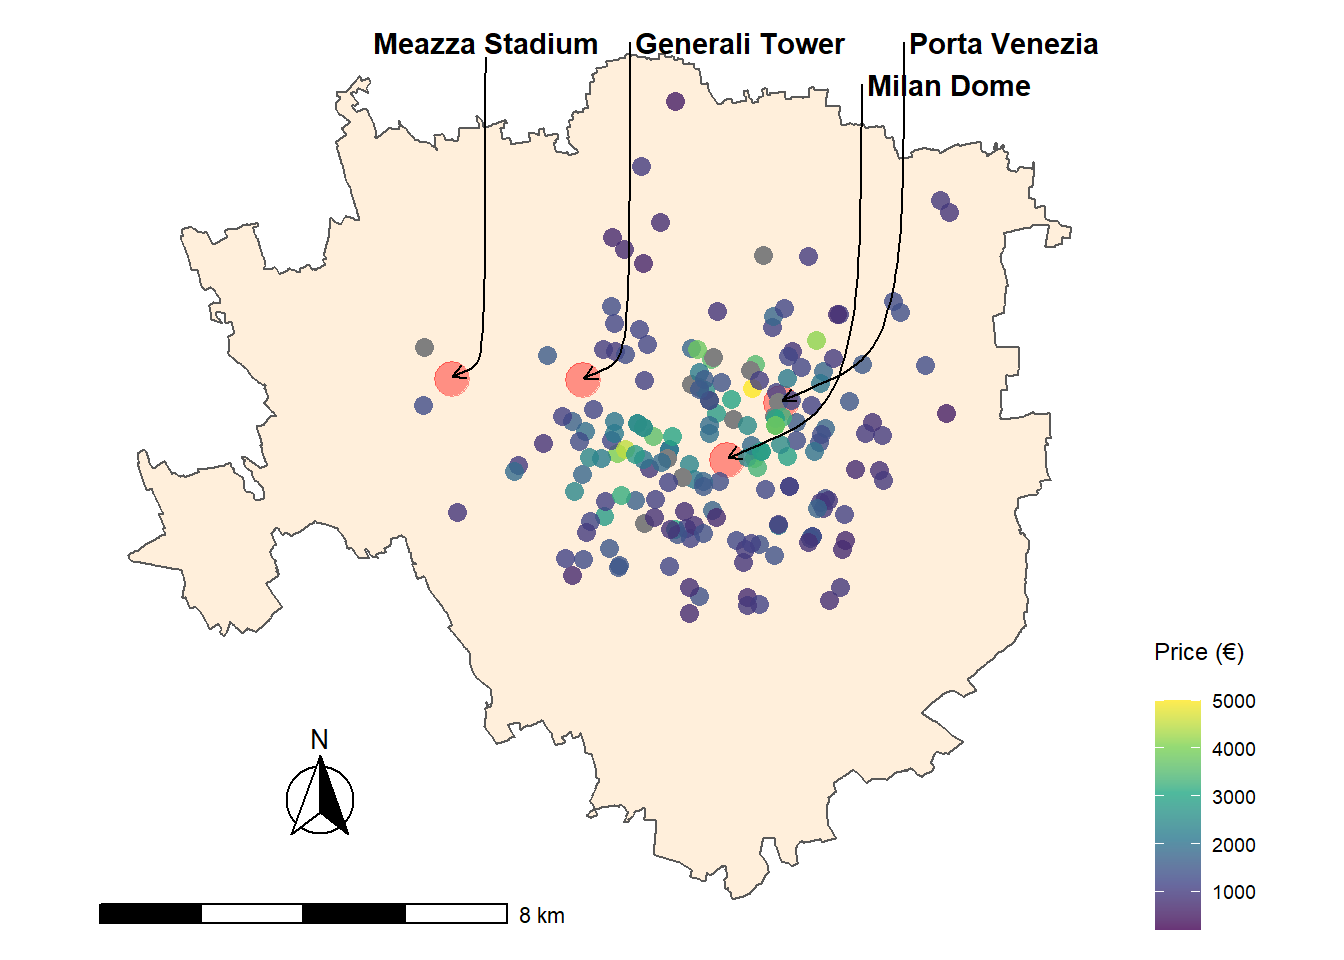
\includegraphics{07-model_fitting_files/figure-latex/ggmap-1} 

}

\caption{Milan Real Estate data within the Municpality borders, 4 points of interest}\label{fig:ggmap}
\end{figure}

\hypertarget{modelspecandmesh}{%
\section{Model Specification \& Mesh Assessement}\label{modelspecandmesh}}

WIth the aim to harness INLA power a hierarchical LGM need to be imposed. Its definition starts from fitting an exponential family distribution on Milan Real Estate Rental data \(\mathbf{y}\) i.e.~normal distribution:

\[
\mathbf{y}\sim \operatorname{Normal}\left(\boldsymbol\mu, \sigma_{e}^{2}\right)
\]

Then the linear predictor i.e.~the mean, since the function \(\mathrm{g}\left(\boldsymbol\mu\right)\) is identity, is:

\[
\boldsymbol\eta=b_{0}+\boldsymbol x \boldsymbol\beta+\boldsymbol\xi 
\]
where, following the notation in expression \eqref{eq:linearpredictor}, \(\boldsymbol\xi\) is the spatial random effect assigned to the function \(f_1()\), for the set of coviarates \(\boldsymbol{z}=\left(x_{1} = lat,\, x_{2} = long\right)\). \(\boldsymbol\xi\) is also the GMRF defined in\ref{def:gmrf}, as a result it is distributed as a multivariate Normal centered in 0 and whose covariance function is Matérn (fig.~\ref{fig:matern}) i.e.~\(\xi_{i} \sim N\left(\mathbf{0}, \mathbf{Q}_{\mathscr{C}}^{-1}\right)\). The precision matrix \(\mathbf{Q}_{\mathscr{C}}^{-1}\) (see left panel in figure \ref{fig:precisionmat}) is the one that requires to be treated with SPDE and its dimensions are \(n \times n\), in this case when NAs are omitted and after imputation it results in \(192 \times 192\).
\(\boldsymbol\beta\) are the model scraped covariates coefficients.
Then the latent field is composed by \(\boldsymbol{\theta}=\{\boldsymbol{\xi}, \boldsymbol{\beta}\}\). In the end following the traits of the final expression in \ref{GP} the LGM can be reformatted as follows,

\[
\boldsymbol{\mathbf{y}}=\boldsymbol{z} \boldsymbol{\beta}+\boldsymbol{\xi}+\boldsymbol{\varepsilon}, \quad \boldsymbol{\varepsilon} \sim N\left(\mathbf{0},  \sigma^2_{\varepsilon} I_{d}\right)
\]
Priors are assigned as Gaussian vagues ones for the \(\boldsymbol\beta\) coefficients with fixed precision, indeed for the GMRF priors are assigned to the matérn process \(\tilde{\boldsymbol\xi}\) as Penalized in Complexity.
Thus following the steps and notation marked in sec.~\ref{LGM}. the \emph{higher} level eq. \eqref{eq:higher} is constituted by the \textbf{likelihood}, depending on hyper parameters \(\boldsymbol\psi_1 = \{\sigma_{\varepsilon}^2\}\):

\[\pi(\boldsymbol{\mathbf{y}} \mid \boldsymbol{\theta}, \boldsymbol{\psi_1})=\prod_{i\ = 1}^{\mathbf{192}} \pi\left(y_{i} \mid \theta_{i}, \boldsymbol{\psi_1}\right)\]

At the \emph{medium} level eq. \eqref{eq:medium} there exists the \textbf{latent field} \(\pi(\boldsymbol{\theta} \mid \boldsymbol\psi_2)\), conditioned to the hyper parameter , whose only component is the measurement error precision, \(\boldsymbol\psi_2 = \left(\sigma_{\mathscr{\xi}}^{2}, \phi, \nu\right)\):

\[  \pi(\boldsymbol{\theta} \mid \boldsymbol{\psi_2})=(2 \pi)^{-n / 2}| \boldsymbol{Q_{\mathscr{C}}(\psi_2)}|^{1 / 2} \exp \left(-\frac{1}{2} \boldsymbol{\theta}^{\prime} \boldsymbol{Q_{\mathscr{C}}(\psi_2)} \boldsymbol{\theta}\right)\]

In the lower level priors are considered as their joint distribution i.e.~\(\boldsymbol\psi_ =\{ \boldsymbol\psi_1\, \boldsymbol\psi_2\}\). It follows the expression of the joint posterior distribution:

\[
\pi(\boldsymbol{\theta}, \boldsymbol{\psi} \mid \mathbf{y})\propto  \underbrace{\pi(\boldsymbol{\psi})}_{\text {priors}} \times \underbrace{\pi(\boldsymbol\theta \mid \boldsymbol\psi)}_{\text {GMRF}} \times \underbrace{\prod_{i=1}^{\mathbf{192}} \pi\left(\mathbf{y} \mid \boldsymbol\theta, \boldsymbol{\psi}\right)}_{\text {likelihood }}
\]
Then once again the objectives of bayesian inference are the posterior marginal distributions for the latent field and the hyperparameters, which are contained in equation \eqref{eq:finalobj}, for which Laplace approximations in \ref{approx} are employed.

\hypertarget{spdemodeol}{%
\section{Building the SPDE object}\label{spdemodeol}}

SPDE requires to triangulate the domain space \(\mathscr{D}\) as intuited in \ref{spdeapproach}. The function \passthrough{\lstinline!inla.mesh.2d!} together with the \passthrough{\lstinline!inla.nonconvex.hull!} are able to define a good triangulation since no proper boundaries are provided. Four meshes are produced, whose figures are in \ref{fig:meshes}. Triangles appears to be thoroughly smooth and equilateral. The extra offset prevents the model to be affected by boundary effects. However the maximum accessible number of vertices is in \(\operatorname{mesh}_3\) , it seems to have the most potential for this dataset. Critical parameters for meshes are \passthrough{\lstinline!max.edge=c(0.01, 0.02)!} and \passthrough{\lstinline!offset=c(0.0475, 0.0625))!} which in fact mold their sophistication. Further trials have shown that below the lower bound of max.edge of \(0.01\) the function is not able to produce the triangulation.

\begin{figure}

{\centering 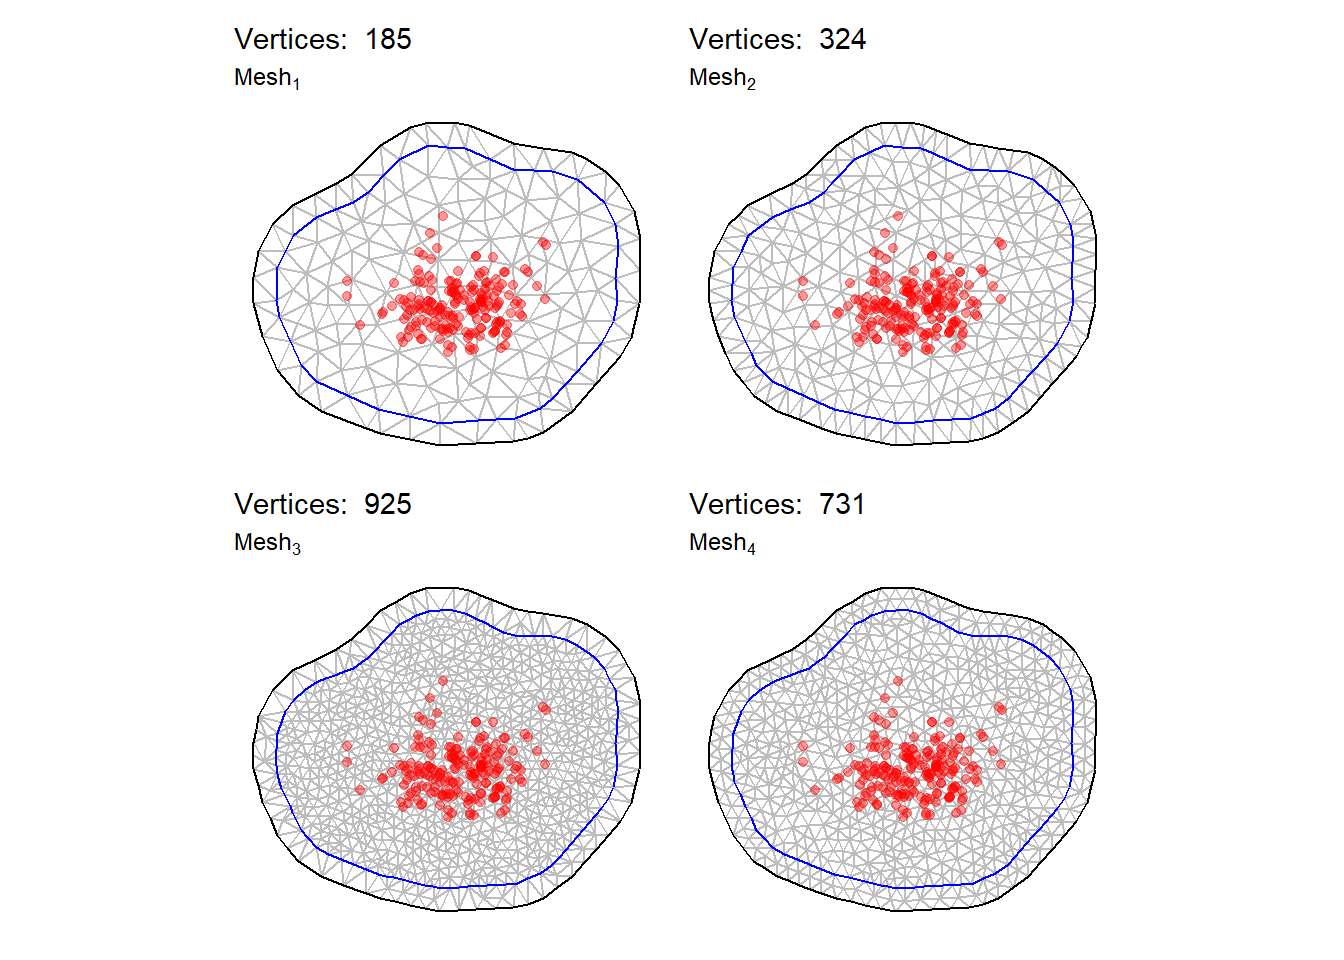
\includegraphics{07-model_fitting_files/figure-latex/meshes-1} 

}

\caption{Left: mesh traingulation for 156 vertices, Right: mesh traingulation for 324 vertices}\label{fig:meshes}
\end{figure}

The SPDE model object is built with the function \passthrough{\lstinline!inla.spde2.pcmatern()!} which needs as arguments the mesh triangulation, i.e.~\(\operatorname{mesh}_3\) and the PC priors \ref{priorsspec}, satisfying the following probability statements: \(\operatorname{Prob}(\sigma_{\varepsilon}^2<3060)< 0.01\) where \(\sigma_{\varepsilon}^2\) is the spatial range desumed in \ref{fig:semivariogram}. And \(\operatorname{Prob}(\tau> 0.9)< 0.05\) where \(\tau\) is the marginal standard deviation (on the log scale) of the field \ref{spatassess}.
As model complexity increases, for instance, a lot of random effects may be discovered in the linear predictor and chances are that SPDE object may get into trouble. As a result the \passthrough{\lstinline!inla.stack!} function recreates the linear predictor as a combination of the elements of the old linear predictor and the matrix of observations. Further mathematical details about the stack are in \citet{Blangiardo-Cameletti}, but are beyond the scope of the analysis.

\hypertarget{model-selection}{%
\section{Model Selection}\label{model-selection}}

Since covariates are many they arouse also many possible combinations of predictors that may better shape complex dynamics. However, there is the possibility to take advantage of several natively implemented ways to use built-in INLA features. As a matter of fact in section \ref{devbased} are presented a set of tools to compare models based on deviance criteria. One of them is DIC which actually balances the number of features applying a penalty when the number of features introduced increases eq. \eqref{eq:dic}.
Consequently a Forward Stepwise Selection \citep{guyon2003introduction} algorithm is designed within the inla function call. One at a time predictors are introduced into the model then results are stored into a dataframe. In the end the most satisfying combination based on DIC is sorted out.

\begin{lstlisting}
#> [1] "condom + totlocali + bagno + cucina + heating + photosnum + floor + sqfeet + fibra_ottica + videocitofono + impianto_di_allarme + reception + porta_blindata WAIC  = -7.532 DIC =-9.001"
\end{lstlisting}

\hypertarget{fit}{%
\section{Parameter Estimation and Results}\label{fit}}

Now the candidate statistical model is fitted rebuilding the stack and calling inla on the final formula i.e.~number of predictors. When the model has run, the conclusions for the random and fixed effects are now discussed.

\begin{table}

\caption{\label{tab:modelfitting}Summary statistics for the top 10 coefficients arranged by descending mean}
\centering
\begin{tabular}[t]{lrrrrr}
\toprule
coefficients & mean & sd & 0.025quant & 0.5quant & 0.975quant\\
\midrule
Intercept & 5.46 & 12.91 & -19.89 & 5.46 & 30.79\\
totlocaliTrilocale & 1.19 & 12.91 & -24.15 & 1.19 & 26.52\\
totlocali5+ & 1.18 & 12.91 & -24.17 & 1.18 & 26.50\\
totlocaliBilocale & 1.09 & 12.91 & -24.25 & 1.09 & 26.42\\
totlocaliQuadrilocale & 1.03 & 12.91 & -24.32 & 1.03 & 26.36\\
\addlinespace
totlocaliPentalocale & 0.97 & 12.91 & -24.38 & 0.97 & 26.29\\
heatingAutonomo, a pavimento, alimentato a pompa di calore & 0.67 & 0.21 & 0.26 & 0.66 & 1.08\\
receptionyes & 0.46 & 0.16 & 0.14 & 0.46 & 0.78\\
heatingCentralizzato, ad aria & 0.33 & 0.17 & 0.00 & 0.33 & 0.66\\
heatingCentralizzato, a pavimento, alimentato a pompa di calore & 0.31 & 0.15 & 0.01 & 0.31 & 0.60\\
\bottomrule
\end{tabular}
\end{table}

Since the models coefficients are many i.e.66 the analysis will concentrate on the most interesting ones. Looking at table \ref{tab:modelfitting} where coefficients are arranged by descending mean, the posterior mean for the intercept, rescaled back from log, is truly quite lofty, affirming that the average house price is 235.1 €.
Moreover being a ``Trilocale'' or ``Bilocale'', as pointed out in \ref{mvp}, brings a monthly extra profit respectively of 3.29 € and 2.97 €. However standard deviations are quite high.
Unsurprisingly the covariate condominium is positively correlated with the response price but its effect is not very tangible. This might imply that pricier apartments expect in mean the same condominium cost as the cheaper ones.
Moreover one feature strongly requested and paid is having a floor heating system, regardless of it is autonomous or centralized.
INLA is able to output the mean and the standard deviation of measurement precision error in \(\psi_2\) i.e.~\(1 / \sigma_{\varepsilon}^{2}\), note that the interpretation is different from variance. In figure \ref{fig:summhyper} are plotted the respective marginal hyper parameter distributions for \(\boldsymbol\psi\).

\textbackslash begin\{table\}

\textbackslash caption\{(\#tab:table\_hyper)Summary statistics for Hyper Parameters\}
\centering

\begin{tabular}[t]{lrr}
\toprule
hyper-param & sd & mode\\
\midrule
Precision for the Gaussian observations & 4.3460742 & 30.350547\\
Theta1 for site & 0.3729812 & -3.570613\\
Theta2 for site & 0.4993020 & 3.913943\\
\bottomrule
\end{tabular}

\textbackslash end\{table\}

\begin{figure}

{\centering 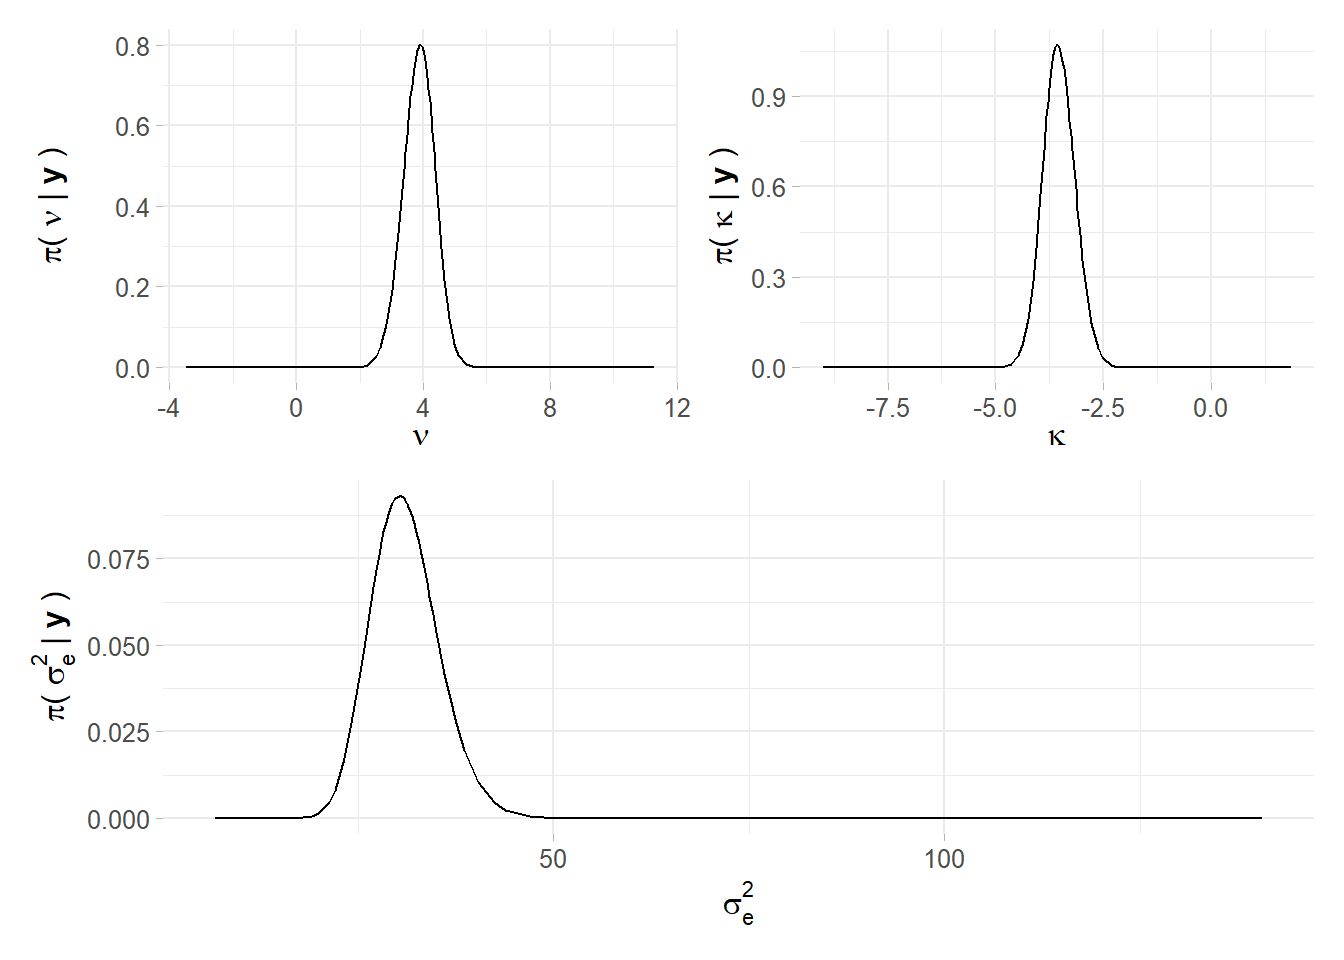
\includegraphics{07-model_fitting_files/figure-latex/summhyper-1} 

}

\caption{Marginal Hyper Parameter distributions for each element of Psi}\label{fig:summhyper}
\end{figure}

\hypertarget{plot-gmrf}{%
\section{Plot GMRF}\label{plot-gmrf}}

Finally, it might be of interest to look at the latent field into the spatial field. The investigation can inform about possible omitted variables, i.e.~how much variance the predictors are not able to capture in the response variable. From plot \ref{fig:pltgmrf}, for which it is chosen a grid of \(150 \times 150\) points, seems that the variance is correctly explained evidencing also three distinctive darker and relatively cheaper areas.

\begin{figure}

{\centering 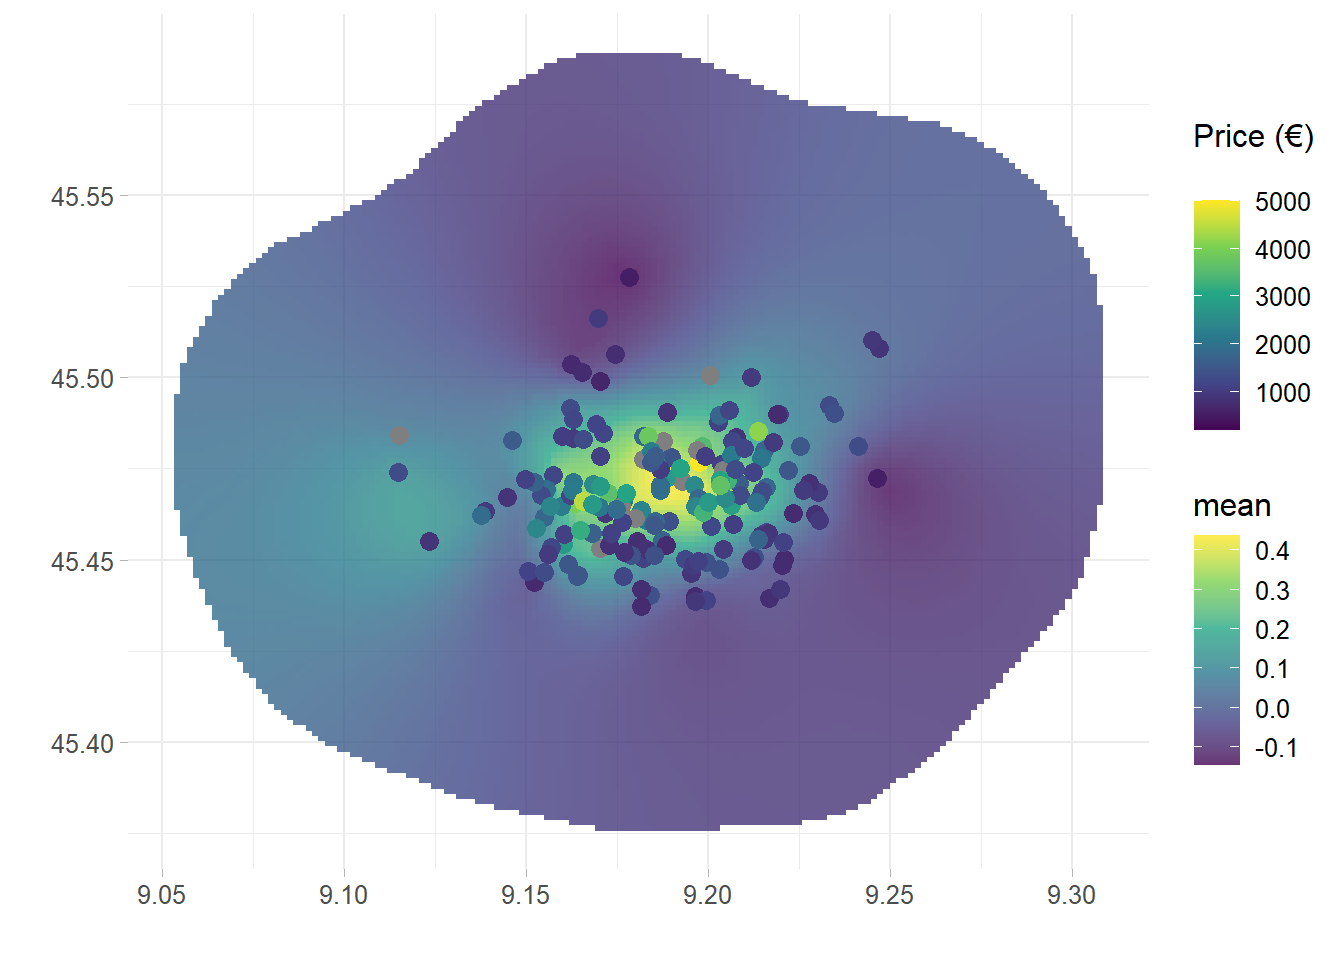
\includegraphics{07-model_fitting_files/figure-latex/pltgmrf-1} 

}

\caption{Gaussian Markov Random field of the final model projected onto the spatial field}\label{fig:pltgmrf}
\end{figure}

\hypertarget{spatial-model-criticism}{%
\section{Spatial Model Criticism}\label{spatial-model-criticism}}

The model on the basis of the PIT \ref{predbase} does not seems to show consistent residual trend nor failures (meaning bizarre values in relation to the others) i.e.~\$fails = \$ 8 outliers. The fact that the distribution is seemingly Uniform \ref{fig:modelcpo} tells that the model is correctly specified. This is summarized by the LPML statistics which accounts for the negative log sum of each cross validate CPO, obtaining 6.681.

\begin{figure}

{\centering \includegraphics{07-model_fitting_files/figure-latex/modelcpo-1} 

}

\caption{PIT cross validation statistics on $model_final$}\label{fig:modelcpo}
\end{figure}

\hypertarget{spatial-prediction-on-a-grid}{%
\section{Spatial Prediction on a Grid}\label{spatial-prediction-on-a-grid}}

A gridded object is required in order to project the posterior mean onto the domain space. Usually these operations are very computationally expensive since grid objects size can easily touch \(10^4\) to \(10^6\) points. For the purposes of spatial prediction, it is considered a grid of \(10km \times 10km\) with \(100 \times 100\) grid points. The intention is to chart the price smoothness given the prediction grid, alongside the corresponding uncertainty i.e.~the standard error.
Higher prices in \ref{fig:predgrid} are observed nearby the points of interest in \ref{ggmap}, however the north-ovest displays lower monthly prices. The variance is ostensibly considerable within the domain and unsurprisingly decreases where data is more dense.

\begin{figure}

{\centering \includegraphics{07-model_fitting_files/figure-latex/predgrid-1} 

}

\caption{Prediction on predictive posterior mean a 122X122 grid overlapped with the Mesh3}\label{fig:predgrid}
\end{figure}

\hypertarget{conclusions}{%
\chapter{Conclusions}\label{conclusions}}

Ideally the entire work can be partitioned in two different pieces i.e.~API and Spatial modeling communicating through a common language: data and offering an end-to-end project. For what it concerns the API it consistently delivers data and avoids of all sorts of failures. From some of the statistics proposed throughout the analysis (\ref{parallelscraping}), webscarping general performances are quite high in term of API response time, on which some further analysis are conducted. Results communicate that for 250 data points (6 columns per 10 web pages scrapped) the time taken for the first endpoint i.e.~\emph{scrapefast} is 5 seconds in the very first interrogation (compatible with the background sessions openings \ref{parallelscraping}). For all the following queries it requires a mean time of approximately 1.2 sec.~The behavior is not well understood since the delay happens also for all the new queries even though sessions are already running in background (i.e.~close on exit from application). The time spent might be attributed to a bottleneck caused in some helpers function, but the traceback has not been pursued yet. For larger amount of data (i.e.~2500 observation) the running time behaves linearly and the resulting response mean time is approximately 15 secs. Note that when arguments are the same the cache is able to return back data requested in no time.
Indeed for what concerns the second endpoint i.e.~\emph{completescrape} for 250 data points (40 covariates including the spatials one) the time spent is 15 secs, and for bigger datasets it will occupy a couple of minutes. Results are summarized in table below.
Under the security umbrella no malicious attacks have been registered since the is its is being OPA (Open Public API), this was also due to the sought-after anonymity of the project. API Logs have registered in 4 months span time a timid usage from open source contributors and curious people which based on th query received tested the service. NGINX did its job with credentials even though it has never been required to load balance the api traffic since there were not traffic at all. Anyway the worst case scenario is accounted thanks to loadtest that has clearly shown which is the maximum treshold that the api handles previous crashing. In the end legal profiles have not been raised, thankfully. However given the progressive importance of web scraping and its market capitalization it is expected that major players will take precautions and manage their servers with stricter rules. The market orientation according to the author seems to subdivide players into two categories, the bigger ones (\href{https://www.idealista.com/}{Idealista.com}, \href{https://www.trovit.it/}{trovit}) operating on more than one country i.e.~Italy, Spain for which barriers have already been raised. And the smaller ones i.e.~\href{https://www.casa.it/}{casa.it} \href{https://www.soloaffitti.it/}{soloaffitti.it} whose domain is ending with .it and whose barriers are not existing yet. Though jurisprudential guidelines lately have judged in favor of scrapers preventing the contestor from disallowing the access to their platform. As a matter of fact both of the parts need to meet halfway since there are a palette of greys between who is sneaking sensible data and who is benefiting from open data and be to the advantage of others through its externalities. Aside from this fact a major effort was put into making the disseration documents portable (\ref{Infrastructure}) and available into a \href{https://niccolosalvini.github.io/thesis/}{website}, strechting to the maximun the concept of collaborative environment and open source. As a curiosity the author has also monitored through time the website audience embedding Google Analytics. What it has been observed in 5 months (Sep to Jan) is a modest international crowd coming from three continents (central panel fig.~\ref{fig:gaanalytics}) the most operating on desktop devices, even though a substantial slice browsed the thesis from their smartphone. The top location was Florence (hometown) with 19 access, immediately followed by Rome, Milan and Quincy (Massachusetts, USA).

\begin{figure}
\centering
\includegraphics{images/analytics_dashbboard.jpg}
\caption{\label{fig:gaanalytics}Google Analyitics Dashoaboard for site logs, author's source}
\end{figure}

INLA unveals incredible results in terms of fitting time and capacity to make the most of its flexibility. Moreover open source projects that are integrating INLA are closing the gap in the learning curve since many tutorials and software can assist the researcher. What it might be for sure welcomed is a more \passthrough{\lstinline!\{tidyverse\}!} orientation and integration of new spatial data packages such as \passthrough{\lstinline!sf!} instead of the superseded \passthrough{\lstinline!sp!}. The model fitted wan not deeply nested since it includes only the random spatial effects, limiting the number of hyper parameters to 4. With that said INLA was able to fit the spatial model astonishingly quick, the cross validated model selection, which evaluates 31 different models has been fitted in \(\approx 5\) minutes. However it is presumed that as soon as the dimensions of data increases then performances are going to be deteriorated. Triangulation has reached a sufficient amount of sophistication even though for unexplained reasons for certain values mesh computing does not converge. The model selection has clearly pointed out that many of the covariates are negligible to the price.
For what concerns the results of the spatial model it is ascertained that prices deeply depends on the location, moreover besides where prices are higher, it would be better concentrating on where are cheaper. As a matter of fact it seems that prices in posterior prediction are aligned on top of a longitudinal straight line traversing the map from south east through the north west. That suggests that cheaper rents are located throughout the orthogonal directrix.

\hypertarget{appendix}{%
\chapter*{Appendix}\label{appendix}}
\addcontentsline{toc}{chapter}{Appendix}

\hypertarget{triangular}{%
\section{SPDE and Triangulation}\label{triangular}}

In order to fit LGM type of models with a spatial component INLA uses SPDE (Stochastic Partial Differential Equations) approach.
Suppose that is it given have a continuous Gaussian random process (a general continuous surface), what SPDE does is to approximate the continuous process by a discrete Gaussian process using a triangulation of the region of the study. Let assume to have a set of points defined by a CRS system (Latitude and Longitude, Easthings and Northings), and let assume that the object of the analysis is to estimate a spatially continuous process. Instead of exploiting this property as a whole, it is estimated the process only at the vertices of this triangulation. This requires to put a Triangulation of the region of the study on top the the process and the software will predict the value of the process at its vertices, then it interpolates the rest of the points obtaining a ``scattered'' surface.

\begin{figure}
\centering
\includegraphics{appendix_images/appendix_triangularization.jpg}
\caption{\label{fig:triang}Triangulariation weights and associated process value, \citet{YT:paumoraga} source}
\end{figure}

Imagine to have a point a location X laying inside a triangle whose vertices are \(S_1, S_2 and S_3\). SPDE operates by setting the values of the process at location x equal to the value of the process at their vertices with some weights, and the weights are given by the \emph{Baricentric coordinates (BC)}. BC are proportional to the area at the point and the vertices. Let assume to have a piece of Triangulation \(\boldsymbol{A}\) and let assume that the goal is to compute the value at location X. X, as in formula above \(\boldsymbol{A}\), would be equal to \(S_1\), multiplied by the area \(A_1\) dived by the whole triangle area (\(\boldsymbol{A}\)) + \(S_2\) multiplied by the area \(A_2\) divided by \(\boldsymbol{A}\) + \(S_3\), multiplied by the area \(A_3\) dived by (\(\boldsymbol{A}\). This would be the value of the process at location X given the triangulations (number of vertices). SPDE is actually approximating the value of the process using a weighted average of the value of the process at the triangle vertices which ir proportional to the area of the below triangle.
In order to do this within INLA \ref{inla} it is needed also a \emph{Projection Matrix} , figure \ref{fig:projmat}. The Projection matrix maps the continuous GRMF (when it is assumed a GP) from the observation to the triangulation. It essentially assigns the height of the triangle for each vertex of the Triangulation to the process. Matrix \(\mathcal{A}\), whose dimensions are \(\mathcal{A_{ng}}\). It has \(n\) rows a \(g\) columns, where \(n\) is the number of observations and \(g\) is the number of vertices of the triangulation. Each row has possibly three non-0 values, right matrix in figure \ref{fig:projmat}, and the columns represent the vertices of the triangles that contains the point. Assume to have an observation that coincides with a vertex \(S_1\) of the triangle in \ref{fig:triang}, since the point is on top of the vertex (not inside), there are no weights (\(A_1 = \mathcal{A}\)) and 1 would be the value at \(A_{(1,1)}\) and 0 would be the rest f the values in the row. Now let assume to have an observation coinciding with \(S_3\) (vertex in position 3), then the result for \(A_{(2,3)}\) would be 1 and the rest 0. Indeed when tha value is X that lies within one of the triangles all the elements of the rows will be 0, but three elements in the row corresponding of the p osition of the vertices \(1 = .2, 2 = .2 and g = .6\), as a result X will be weighted down for the areas.

\begin{figure}
\centering
\includegraphics{appendix_images/appendix_proj.jpg}
\caption{\label{fig:projmat}Projection Matrix to map values from tringulation back to the GP, \citet{YT:paumoraga} surce}
\end{figure}

\hypertarget{laplaceapprox}{%
\section{Laplace Approximation}\label{laplaceapprox}}

\citet{Blangiardo-Cameletti} offers an INLA focused intuiton on how the Laplace approximation works for integrals. Let assume that the interest is to compute the follwing integral, assuming the notation followed throughout the analysis:

\[
\int \pi(x) \mathrm{d} x=\int \exp (\log f(x)) \mathrm{d} x
\]
Where \(X\) is a random variable for which it is specified a distribution function \(\pi\). Then by the Taylor series expansions \citep{taylorseries} it is possible to represent the \(\log \pi(x)\) evaluated in an exact point \(x = x_0\), so that:

\begin{equation}
\log \pi(x) \approx \log \pi\left(x_{0}\right)+\left.\left(x-x_{0}\right) \frac{\partial \log \pi(x)}{\partial x}\right|_{x=x_{0}}+\left.\frac{\left(x-x_{0}\right)^{2}}{2} \frac{\partial^{2} \log \pi(x)}{\partial x^{2}}\right|_{x=x_{0}}
\label{eq:secondordexpan}
\end{equation}

Then if it is assumed that \(x_0\) is set equal to the mode \(x_*\) of the distribution (the highest point), for which \(x_{*}=\operatorname{argmax}_{x} \log \pi(x)\), then the first order derivative with respect to \(x\) is 0, i.e.~\(\left.\frac{\partial \log f(x)}{\partial x}\right|_{x=x_{*}}=0\). That comes natural since once the function reaches its peak, i.e.~the max then the derivative in that point is 0. Then by leaving out the first derivative element in eq. \eqref{eq:secondordexpan} it is obtained:

\[
\log \pi(x) \approx \log \pi\left(x_{*}\right)+\left.\frac{\left(x-x_{*}\right)^{2}}{2} \frac{\partial^{2} \log \pi(x)}{\partial x^{2}}\right|_{x=x_{*}}
\]

Then by integrating what remained, exponantiating and taking out non integrable terms,

\begin{equation}
\int \pi(x) \mathrm{d} x \approx \exp \left(\log \pi\left(x_{*}\right)\right) \int \exp \left(\left.\frac{\left(x-x_{*}\right)^{2}}{2} \frac{\partial^{2} \log \pi(x)}{\partial x^{2}}\right|_{x=x_{*}}\right) \mathrm{d} x
\label{eq:integraltay}
\end{equation}

At this point it might be already intuited the expression \eqref{eq:integraltay} is actually the density of a Normal. As a matter of fact, by imposing \(\sigma^{2}_{*}=-1 /\left.\frac{\partial^{2} \log f(x)}{\partial x^{2}}\right|_{x=x_{*}}\), then expression \eqref{eq:integraltay} can be rewritten as:

\begin{equation}
\int \pi(x) \mathrm{d} x \approx \exp \left(\log \pi\left(x_{*}\right)\right) \int \exp \left(-\frac{\left(x-x_{*}\right)^{2}}{2 \sigma^{2}_{*}}\right) \mathrm{d} x
\label{eq:rearrangeintr}
\end{equation}

Furthermore the integrand is the \emph{Kernel} of the Normal distribution having mean equal to the mode \(x_*\) and variance specified as \(\sigma^{2}_{*}\). By computing the finite integral of \eqref{eq:rearrangeintr} on the closed neighbor \([ \alpha, \beta]\) the approximation becomes:

\[
\int_{\alpha}^{\beta} f(x) \mathrm{d} x \approx \pi\left(x_{*}\right) \sqrt{2 \pi \sigma^{2^{*}}}(\Phi(\beta)-\Phi(\alpha))
\]
where \(\Phi(\cdot)\) is the cumulative distribution function corresponding value of the Normal disttribution in eq. \eqref{eq:rearrangeintr}.

For example consider the Chi-squared \(\chi^{2}\) density function (since it is easily differentiable and Gamma \(\Gamma\) term in denominator is constant). The following quantities of interest are the \(\log \pi(x)\), then the \(\frac{\partial \log \pi(x)}{\partial x}\), which has to be set equal to 0 to find the integrating point, and finally \(\log \pi(x)\) \(\frac{\partial^2 \log \pi(x)}{\partial x^2}\). The \(\chi^{2}\) pdf, whose support is \(x \in \mathbb{R}^{+}\) and whose degrees of freedom are \(k\):

\[
\chi^{2}(x,k)=\frac{x^{(k / 2-1)} e^{-x / 2}}{2^{k / 2} \,\, \Gamma\left(\frac{k}{2}\right)}, x \geq 0
\]

for which are computed:

\[
\log f(x)=(k / 2-1) \log x-x / 2
\]
Ths single variable \emph{Score Function} and the \(x_{*}=\operatorname{argmax}_{x} \log \pi(x)\),

\begin{equation}
\begin{aligned} 
  &\frac{\partial \log \pi(x)}{\partial x}= \frac{(k/2 -1)}{x} - \frac{1}{2} =0 \quad \text {solving for 0 }\\
  &(k/2-1) = x/2\quad \text {moving addends}\\
  &x_* = (k-2) 
\end{aligned}
\end{equation}

And the \emph{Fisher Information} in the \(x_*\) (for which it is known \(\sigma^{2}_*=-1 / f^{\prime \prime}(x)\))

\begin{equation} 
\begin{split}
  &\frac{\partial^2 \log \pi(x)}{\partial x^2}=-\frac{(k / 2-1) }{x^{2}} \quad \text {substituting} \,\,x_* \\
  &= -\frac{(k / 2-1) }{(k-2)^{2}} = - \frac{2(k/2-1)}{2(k-2)^{2}} \quad \text {multiply by 2 } \\
  &=-  \frac{(k-2)}{2(k-2)^{2}} = 2(k-2)  = \sigma^{2}_*\quad \text {change of sign and inverse }
\end{split}
\end{equation}

finally,

\[
\chi^{2} \stackrel{L A}{\sim} N\left(x_*=k-2, \sigma^{2}_*=2(k-2)\right)
\]
Assuming \(k = 8, 16\) degrees of freedom \(\chi^{2}\) densities against their Laplace approximation, the figure \ref{fig:laplacevisual} displays how the approximations fits the real density. Integrals are computed in the case of \(k = 8\) in the interval \((5, 7)\), leading to a very good Normal approximation that slightly differ from the orginal CHisquared. The same has been done for the \(k = 16\) case, whose interval is \((12, 17)\) showing other very good approximations. Note that the more are the degrees of freedom the more the chi-squared approximates the Normal leading to better approximations.

\begin{figure}

{\centering \includegraphics{98-appendix_files/figure-latex/laplacevisual-1} 

}

\caption{Chisquared density function with parameter $k = 8$ (top) and $k = 16$ (down) solid line. The point line refers to the corresponding Normal approximation obtained using the Laplace method}\label{fig:laplacevisual}
\end{figure}

\[
\pi(\boldsymbol{\psi}) \quad \boldsymbol{\psi}= \boldsymbol{\psi_1}, \boldsymbol{\psi_2}
\]

  \bibliography{refs.bib,Rpackages.bib}

\end{document}
